\documentclass[12pt,a4paper,titlepage,listof=totoc,bibliography=totoc,chapteratlists=0pt]{scrreprt}

\begin{filecontents*}{\jobname.xmpdata}
	\Keywords{VR, IOT, TODO}
	\Title{Unser tolles Thema -- wir sind suppa}
	\Author{Stefan Schwammal, Susi Schwammal}
\end{filecontents*}

\setcounter{tocdepth}{1}

\usepackage[utf8]{inputenc}
\usepackage[T1]{fontenc}
\usepackage{amsmath}
\usepackage{amsfonts}
\usepackage{amssymb}
\usepackage[table]{xcolor}
\usepackage{graphicx}
\usepackage[left=3.50cm, right=2.00cm, top=2.00cm, bottom=2.00cm,foot=1cm]{geometry}
\usepackage[splitrule,hang,flushmargin,multiple,bottom]{footmisc}
\usepackage{lmodern, textcomp}
\usepackage{lmodern}
\usepackage{pdfpages}
\usepackage[ngerman]{babel}
\usepackage{multicol}
\usepackage{subfig}
\usepackage{float}
\usepackage{array,tabularx,booktabs}
\usepackage{ragged2e}
\usepackage{lipsum}
\usepackage{wrapfig}

\newcolumntype{M}[1]{>{\centering\arraybackslash}m{#1}}

\usepackage{enumitem}
\newlist{compactitem}{itemize}{3}
\setlist[compactitem,1]{label=\textbullet, nosep,leftmargin=1.5em,labelwidth=*,align=left}
\setlist[compactitem,2]{label=--, nosep,leftmargin=1.5em,labelwidth=*,align=left}
\setlist[compactitem,3]{label=\textopenbullet, nosep,leftmargin=1.5em,labelwidth=*,align=left}
\newlist{compactenum}{enumerate}{3}
\setlist[compactenum,1]{label=\arabic*., nosep,leftmargin=1.5em,labelwidth=*,align=left}
\setlist[compactenum,2]{label=\alph*., nosep,leftmargin=1.5em,labelwidth=*,align=left}
\setlist[compactenum,3]{label=\roman*., nosep,leftmargin=1.5em,labelwidth=*,align=left}
\newlist{compactdesc}{description}{3}
\setlist[compactdesc]{leftmargin=1.5em,labelwidth=*,align=left}

\usepackage{microtype}

\usepackage[parfill]{parskip}

\definecolor{bluekeywords}{rgb}{0.13,0.13,1}
\definecolor{greencomments}{rgb}{0,0.5,0}
\definecolor{redstrings}{rgb}{0.9,0,0}
\definecolor{lightgray}{gray}{0.9}
\definecolor{lightblue}{rgb}{0.93,0.95,1.0}

\usepackage{listings}

\makeatletter
\lstdefinestyle{lststyle}{
	basicstyle=%
	\ttfamily
	\lst@ifdisplaystyle\scriptsize\fi
}
\makeatother

\renewcommand{\lstlistlistingname}{List of Listings}
% TODO: define other languages as needed
\lstset{language=Python,
numbers=left,               
numberstyle=\tiny,          
showspaces=false,
showtabs=false,
breaklines=true,
lineskip=-1pt,
tabsize=2,
showstringspaces=false,
breakatwhitespace=true,
escapeinside={(*@}{@*)},
commentstyle=\color{greencomments},
keywordstyle=\color{bluekeywords}\bfseries,
stringstyle=\color{redstrings},
style=lststyle,
xleftmargin=17pt,
         framexleftmargin=17pt,
         framexrightmargin=5pt,
         framexbottommargin=4pt
}
\lstset{
morekeywords={base,var,in,out,dynamic,from,where,select,orderby,function,\$,group,by,into,yield,async,await,@,None,self,as,elif,with}
}
\lstdefinelanguage{TypeScript}{
	keywords={typeof, new, true, false, catch, function, return, null, switch, var, if, in, while, do, else, case, break, void, number, string, boolean, module, \$, export, for, this},
	keywordstyle=\color{blue}\bfseries,
	ndkeywords={class, export, boolean, throw, implements, import, this},
	ndkeywordstyle=\color{darkgray}\bfseries,
	identifierstyle=\color{black},
	sensitive=false,
	comment=[l]{//},
	morecomment=[s]{/*}{*/},
	commentstyle=\color{purple}\ttfamily,
	stringstyle=\color{red}\ttfamily,
	morestring=[b]',
	morestring=[b]"
}
\usepackage{caption}
\DeclareCaptionFont{white}{\color{white}}
\DeclareCaptionFormat{listing}{\colorbox[cmyk]{0.43, 0.35, 0.35,0.01}{\parbox{\textwidth}{\hspace{10pt}#1#2#3}}}
\captionsetup[lstlisting]{format=listing,labelfont=white,textfont=white} 
\captionsetup[table]{justification=centering, singlelinecheck=false}

\usepackage{setspace}
\newcommand{\MSonehalfspacing}{%
	\setstretch{1.44}%  default
	\ifcase \@ptsize \relax % 10pt
	\setstretch {1.448}%
	\or % 11pt
	\setstretch {1.399}%
	\or % 12pt
	\setstretch {1.433}%
	\fi
}

\newcommand{\setauthor}[1]{\ohead[]{#1}}

\usepackage[automark]{scrlayer-scrpage}
\pagestyle{scrheadings}
\automark{chapter}
\renewcommand\sectionmark[1]{\markright{\MakeMarkcase {\thesection\hskip .5em\relax#1}}}
\rohead{\ifnum\expandafter\pdfstrcmp\botmark=0 \rightmark\else\leftmark{} --- \rightmark\fi}
\ihead[]{\headmark}
\chead[]{}
\ohead{}
\cfoot[]{}
\ofoot[\pagemark]{\pagemark}
\setheadsepline{.1pt}

\usepackage[hyphens]{url}

\usepackage[a-1b]{pdfx}

\usepackage{hyperref}
\hypersetup{pdfa}

\usepackage[nonumberlist,toc,nopostdot]{glossaries}

\usepackage{chngcntr}
\counterwithout{footnote}{chapter}
\counterwithout{figure}{chapter}
\counterwithout{table}{chapter}
\AtBeginDocument{
	\counterwithout{lstlisting}{chapter}
	\urlstyle{sf}
}
\newcounter{RPages}

\makeatletter
\def\bstctlcite{\@ifnextchar[{\@bstctlcite}{\@bstctlcite[@auxout]}}
\def\@bstctlcite[#1]#2{\@bsphack
	\@for\@citeb:=#2\do{%
		\edef\@citeb{\expandafter\@firstofone\@citeb}%
		\if@filesw\immediate\write\csname #1\endcsname{\string\citation{\@citeb}}\fi}%
	\@esphack}
\makeatother

\clubpenalty=10000
\widowpenalty=10000
\displaywidowpenalty=10000
\interfootnotelinepenalty=10000

\title{Beam VR -- Synchronized Realities}
\author{Quirin Ecker, Florian Beckerle}

\makeindex
\makeglossaries
\begin{document}
\bstctlcite{IEEEexample:BSTcontrol}
\newcommand{\reminder}[1]
{ \textcolor{red}{<[{\bf\marginpar{\mbox{$<==$}} #1 }]>} }
\newcommand{\icode}[1]{\lstinline$#1$}
%\urlstyle{same}
%\setstretch{1.5}
\setstretch {1.433}
\renewcommand{\arraystretch}{1.2}

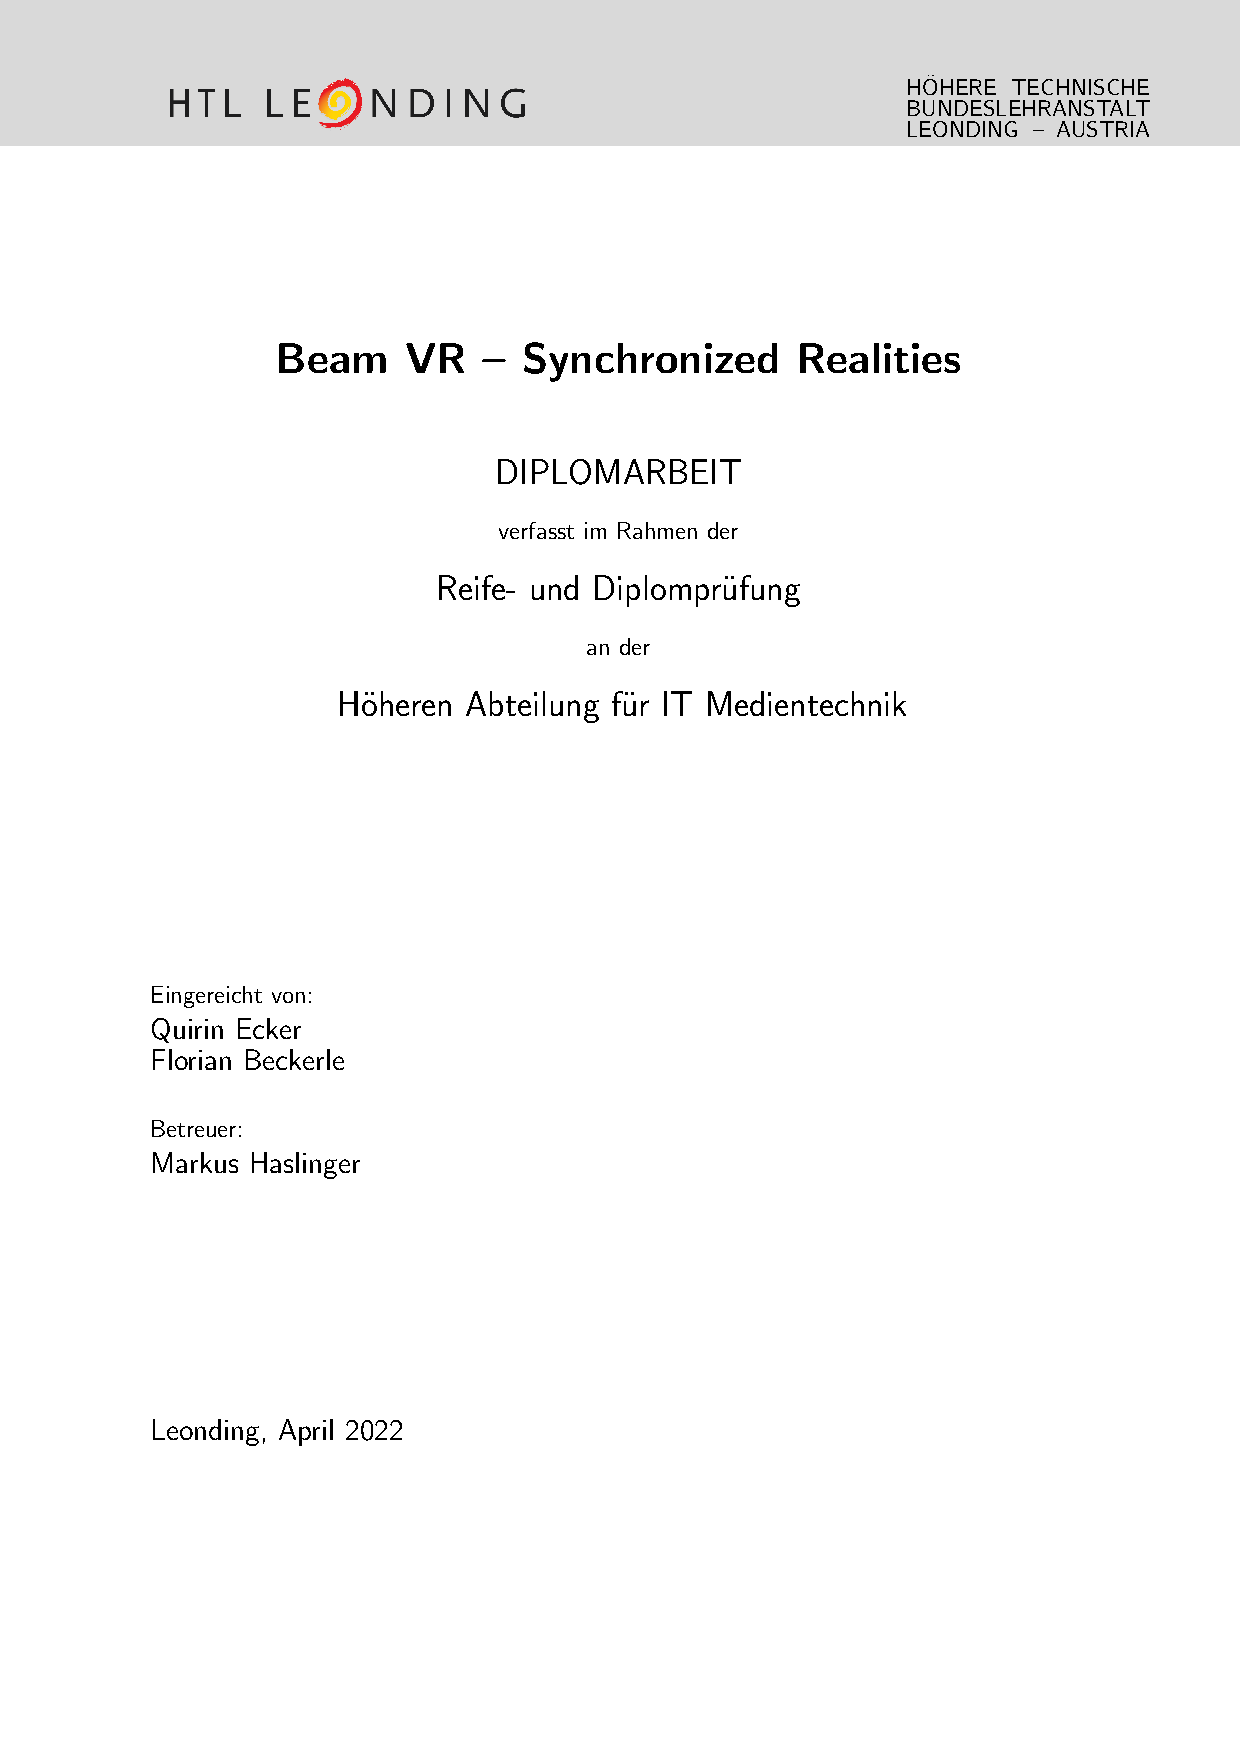
\includepdf{./titlepage/coversheet}
\pagenumbering{Roman}
\newpage
\thispagestyle{empty}
\vspace{3cm}
~ \\ \\
Ich erkläre an Eides statt, dass ich die vorliegende Diplomarbeit selbstständig und ohne fremde Hilfe verfasst, andere als die angegebenen Quellen und Hilfsmittel nicht benutzt bzw. die wörtlich oder sinngemäß entnommenen Stellen als solche kenntlich gemacht habe.

Die Arbeit wurde bisher in gleicher oder ähnlicher Weise keiner anderen Prüfungsbehörde vorgelegt und auch noch nicht veröffentlicht.

Die vorliegende Diplomarbeit ist mit dem elektronisch übermittelten Textdokument identisch.
\vspace{3cm}
% Hier kommt die Unterschrift drüber
\begin{tabbing}
Leonding, April 2022 \hspace{5cm} S. Schwammal \& S. Schwammal
\end{tabbing}
\vspace{10cm}
Zur Verbesserung der Lesbarkeit wurde in diesem Dokument auf eine geschlechtsneutrale Ausdrucksweise verzichtet.
Alle verwendeten Formulierungen richten sich jedoch an beide Geschlechter.
\newpage
\setcounter{page}{1}
\begin{spacing}{1}

    \chapter*{Abstract}

\end{spacing}

\begin{wrapfigure}{r}{0.3\textwidth}

    \begin{center}

        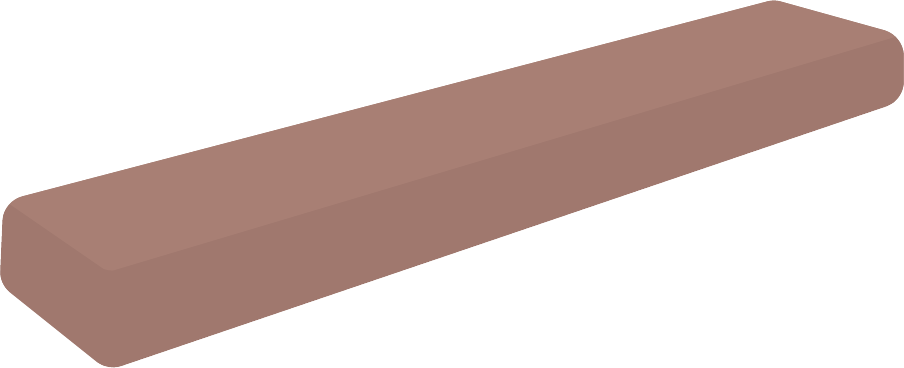
\includegraphics[width=0.2\textwidth]{pics/abstract_picture_1}

    \end{center}

\end{wrapfigure}

Beam VR is a project which aims to give an immersive experience of height.
It consists of a scene on top of a building with a plank, which protrudes from this building.
To increase the immersion we use virtual reality combined with the physical reality (Augmented Virtuality).
In particular the plank exists in the virtual as well as in the physical reality.

With a realistic environment including cars, high skyscrapers and classic new york city sounds we optimize the immersion of the reality.
The objective of the simulation is balancing on the beam without falling off.
Furthermore, the scene can be experienced in three different maps, namely Night, Day and Apocalypse.

\newpage

\begin{spacing}{1}

    \chapter*{Zusammenfassung}

\end{spacing}

\begin{wrapfigure}{r}{0.3\textwidth}

    \begin{center}

        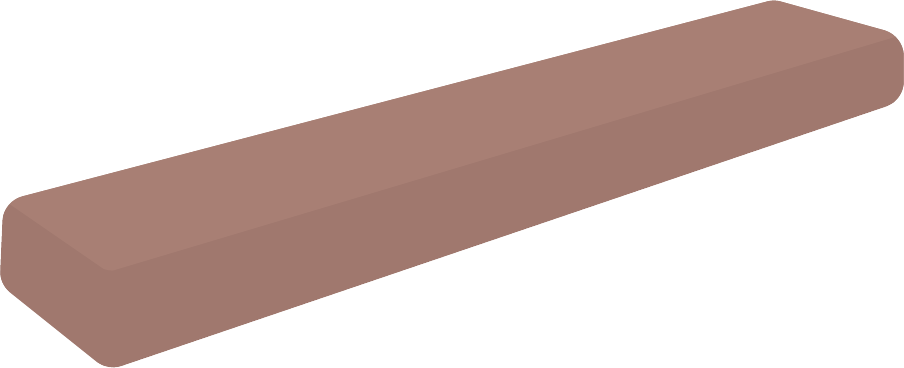
\includegraphics[width=0.2\textwidth]{pics/abstract_picture_1}

    \end{center}

\end{wrapfigure}

Beam VR ist ein Projekt, das darauf abzielt, ein immersives Höhenerlebnis zu vermitteln.
Es besteht aus einer Szene auf einem Gebäude mit einem Brett, das aus diesem Gebäude herausragt.
Um die Immersion zu steigern, verwenden wir Virtual Reality in Kombination mit der physischen Realität (Augmented Virtuality).
Insbesondere das Brett existiert sowohl in der virtuellen als auch in der physischen Realität.

Mit einer realistischen Umgebung aus Autos, hohen Wolkenkratzern und klassischen New-York-City-Sounds optimieren wir das Eintauchen in die Realität.
Ziel der Simulation ist es, auf dem Balken zu balancieren, ohne herunterzufallen.
Darüber hinaus kann die Szene in drei verschiedenen Karten erlebt werden, nämlich Night, Day und Apocalypse.

\begin{spacing}{1}

    \chapter*{Danksagung}

\end{spacing}

An dieser Stelle möchten wir uns bei all jenen bedanken, die durch ihre fachliche, persönliche und finanzielle Unterstützung zum Gelingen dieser Diplomarbeit beigetragen haben.

Besonders möchten wir uns bei Pärtel Lang bedanken, welcher uns netterweise das FinalIK Plugin kostenfrei für diese Arbeit zur Verfügung gestellt hat.

Außerdem sind wir Benjamin Völk und dem Team der Nimbus Cloud für die Bereitstellung ihrer Büroräumlichkeiten sehr dankbar.

Weiters gilt unser Dank Herrn Rudolf Weißensteiner und Frau Ingrid Bauer für das Schneiden, Hobeln, Lackieren und Bereitstellen eines perfekten Holzbalkens.

Schlussendlich möchten wir uns noch bei unserem Betreuer Herrn Professor Haslinger und unserem Abteilungsvorstand Peter Bauer für die fachliche und persönliche Unterstützung während der Erstellung dieser Arbeit bedanken.


\pagestyle{plain}

\renewcommand{\lstlistlistingname}{Quellcodeverzeichnis}

\setcounter{tocdepth}{1}
\tableofcontents
\newpage
\setcounter{RPages}{\value{page}}
\setcounter{page}{0}
\pagenumbering{arabic}
\pagestyle{scrheadings}

\begin{spacing}{1}
\chapter{Einleitung}\label{chapter:introduction}
\end{spacing}
\section{Ausgangssituation}\label{sec: initial_situation}

Es gibt bereits viele VR Applikation, aber was ist genau eine VR Applikation.
Es gibt viele Definitionen für VR ausgeschrieben Virtual Reality.
In dieser Arbeit sprechen wir über die Wirklichkeit welche durch ein head mounted display, oder umgangssprachlich auch eine VR-Brille angezeigt wird.
Somit bezeichnet eine VR Application eine Software, welche in der VR-Brille läuft.

Von diesen VR Applikationen gibt es schon einige.
Die meisten werden im Bereich Videospiele verwendet nach einer Statistik aus Deutschland im Jahre 2021, bei welcher Personen mit einer VR-Brille oder head mounted display befragt worden sind.
Siehe Abbildung~\ref{fig:statistic_usage_vr}

\begin{figure}
    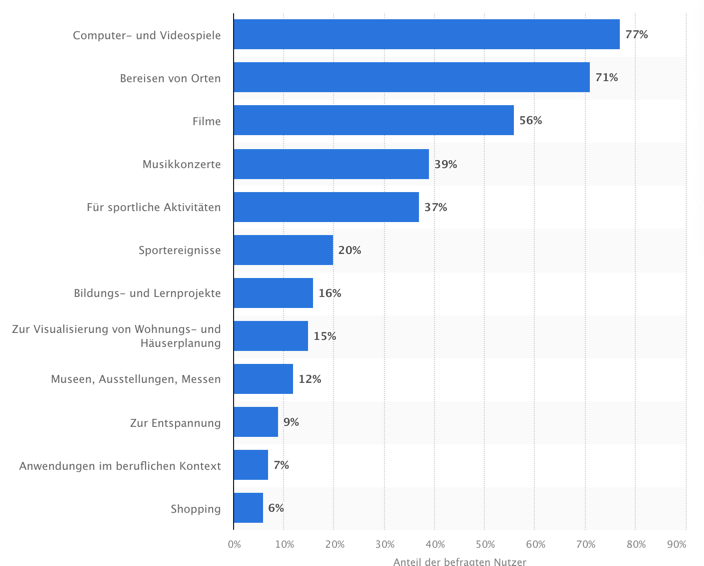
\includegraphics[scale=0.5]{pics/statistic_usage_vr}
    \caption{Anwendungsgebiete VR}
    \label{fig:statistic_usage_vr}
\end{figure}

Bei diesen VR Applikationen ist meist der Kopf getrackt und vielleicht auch Hände, Füße und Hüften.
Interconversions sind meistens aber die weitere interaktion mit der Umgebung.
Setzt einer sich auf einen Sessel wird er durchfliegen, außer er steht auch in der realen Wirklichkeit dort.

\section{Zielsetzung}\label{sec: objective}

Das Ziel von Beam VR ist die physische Realität und die virtuelle Realität zu kombinieren.
Im Falle Beam VR benützen wir hier einen Balken, welcher von einem Hochhaus wegsteht.
Dieser Balken soll in der physischen Realität und in der virtuellen Realität existieren und die gleiche Position einehmen.
Dadurch soll die Immersion entstehen, dass man wirklich auf einem Balken steht, welcher von einem Hochhaus wegsteht.
Auch, wenn man nur in seinem Wohnzimmer oder auch woanders ohne Gefahren auf einem Balken steht.
Beam VR ist nicht der Erfinder dieses Konzeptes.
Mehr dazu gibt es in der kommenden Umfeldanalyse.



\begin{spacing}{1}
\chapter{Umfeldanalyse}
\end{spacing}
% To Do
% Allgemeinerer Start           |
% Quellen nach jedem Absatz     |
% Rechtschreibung :(            |
%

Heutzutage kommen sich die virtuelle und die realle Realität immer näher.
Angefangen von Virtual Reality, wo sich der Benutzer mithilfe einer VR-Brille in eine fiktive Welt begeben kann.
Bis hin zu Augmented Reality, in welcher virtuelle Gegenstände und Strukturen in der reallen Welt angezeigt werden können.
Es gibt neben BeamVR auch noch viele andere verschiedene M\"oglichkeiten um diese Konzepte umsetzen zu können.


%Das Konzept der Synchronisation von einem Gegenstand über den zwei besprochenen Realitäten ist nicht neu.
%Einer der bekanntesten Implementierungen des Konzepts ist Richie's Plank Experience.

\section{Richie's Plank Experience}
\label{sec:richiesplankexperience}
Ein Projekt welches zu einem Teil das gleiche Thema wie BeamVR behandelt, heißt Richie's Plank Experience, welches von TOAST VR PTY. LTD. entwickelt wurde.
Es handelt sich um ein Virtual Reality Spiel, dass auf der PlayStation 4, Oculus Quest und f\"ur Microsoft Windows verf\"ugbar ist.
Bei der Playstation wird auf das Sony exclusive PlayStation VR zur\"uckgegriffen, während auf Windows entweder eine HTC Vive VR Brille oder die Valve Index verwendet werden kann.
~\cite{ToastGames_2021}

\subsection{Spielmodi}
\label{sec:richiesplankexperience_modes}
Richie's Plank Experience bietet dabei mehrere verschiedene Features in Form von Spielmodi an.
Diese Modi werden dem Spieler (\"ahnlich wie bei einer Stockwerkauswahl) in einem Aufzug dargestellt.
Wenn der Spieler einen Modus ausgewählt hat, fährt der Aufzug auf das Hochhausdach.
Dort befindet sich dann der entsprechende Aufbau für den Modus.
Zur Verfügung stehen hierbei die Modi Plank, Sky Brush, Ground, Hero Academy und der Easter Egg Modus Nightmare.
~\cite{ToastGames_2021_Steam}

Im ersten Modus, welcher Plank genannt wird, befindet sich der Spieler weit oben auf einem Hochhaus.
Nach der Auswahl wird angeboten, dass sich am Ende des Balkens eine Belohnung befindet.
Man kann zwischen einem leeren Balken, Kuchen, Donuts und Kuchen mit darin versteckten Spinnen auswählen.
Nun befindet sich vor dem Aufzug nur mehr der Balken mit der vorher getroffenen Belohnung und rundherum der Abgrund.
Die Donuts und die beiden Kuchen können entweder gegessen oder heruntergeworfen werden.
~\cite{ToastGames_2021_Steam}

In Sky Brush kann der Spieler, mithilfe eines kleinen Jetpacks, frei durch die Stadt fliegen.
Dabei wird eine Rauch-Spur hinterlassen welche, wie der Name des Modus schon andeutet, wie ein Pinsel in den Himmel malt.
Nun kann der Spieler, nach eigenem Belieben, verschiedene Kunstwerke erschaffen und betrachten.
~\cite{ToastGames_2021_Steam}

Bei Hero Academy kann der Spieler wieder zwischen mehreren Optionen auswählen.
Bei Fire Deck spielt man einen Superhelden welcher durch die Stadt fliegt und Feuer auf Häusern löschen muss.
Bei Air-Race fliegt man mit den Jetpacks durch Ringe welche als Checkpoints für ein Rennen dienen.
Wurden alle Ringe in richtiger Reihenfolge durchflogen, hat man das Rennen geschafft.
~\cite{ToastGames_2021_Steam}

Im geheimen Modus Nightmare, welcher mithilfe des Codes 666 erreicht werden kann, erlebt der Spieler eine kleine Abfolge von gruseligen Ereignissen.
~\cite{ToastGames_2021_VivePort}

\subsection{Setup}
\label{sec:richiesplankexperience_setup}

Damit man diese Modi, vor allem den Plank Modus, mit einem realen Balken spielen kann, muss mithilfe des Setups der Balken kalibriert werden.
Hierfür wird der Balken etwa in der Mitte der VR-Spielfläche platziert.
Nun sollten beide VR-Controller auf jeweils einem Ende des Balkens platziert werden, wie man auf der Grafik sehen kann.
\ref{fig:beam_length_measurement} %Balken Länge Einstellen

\begin {figure}
    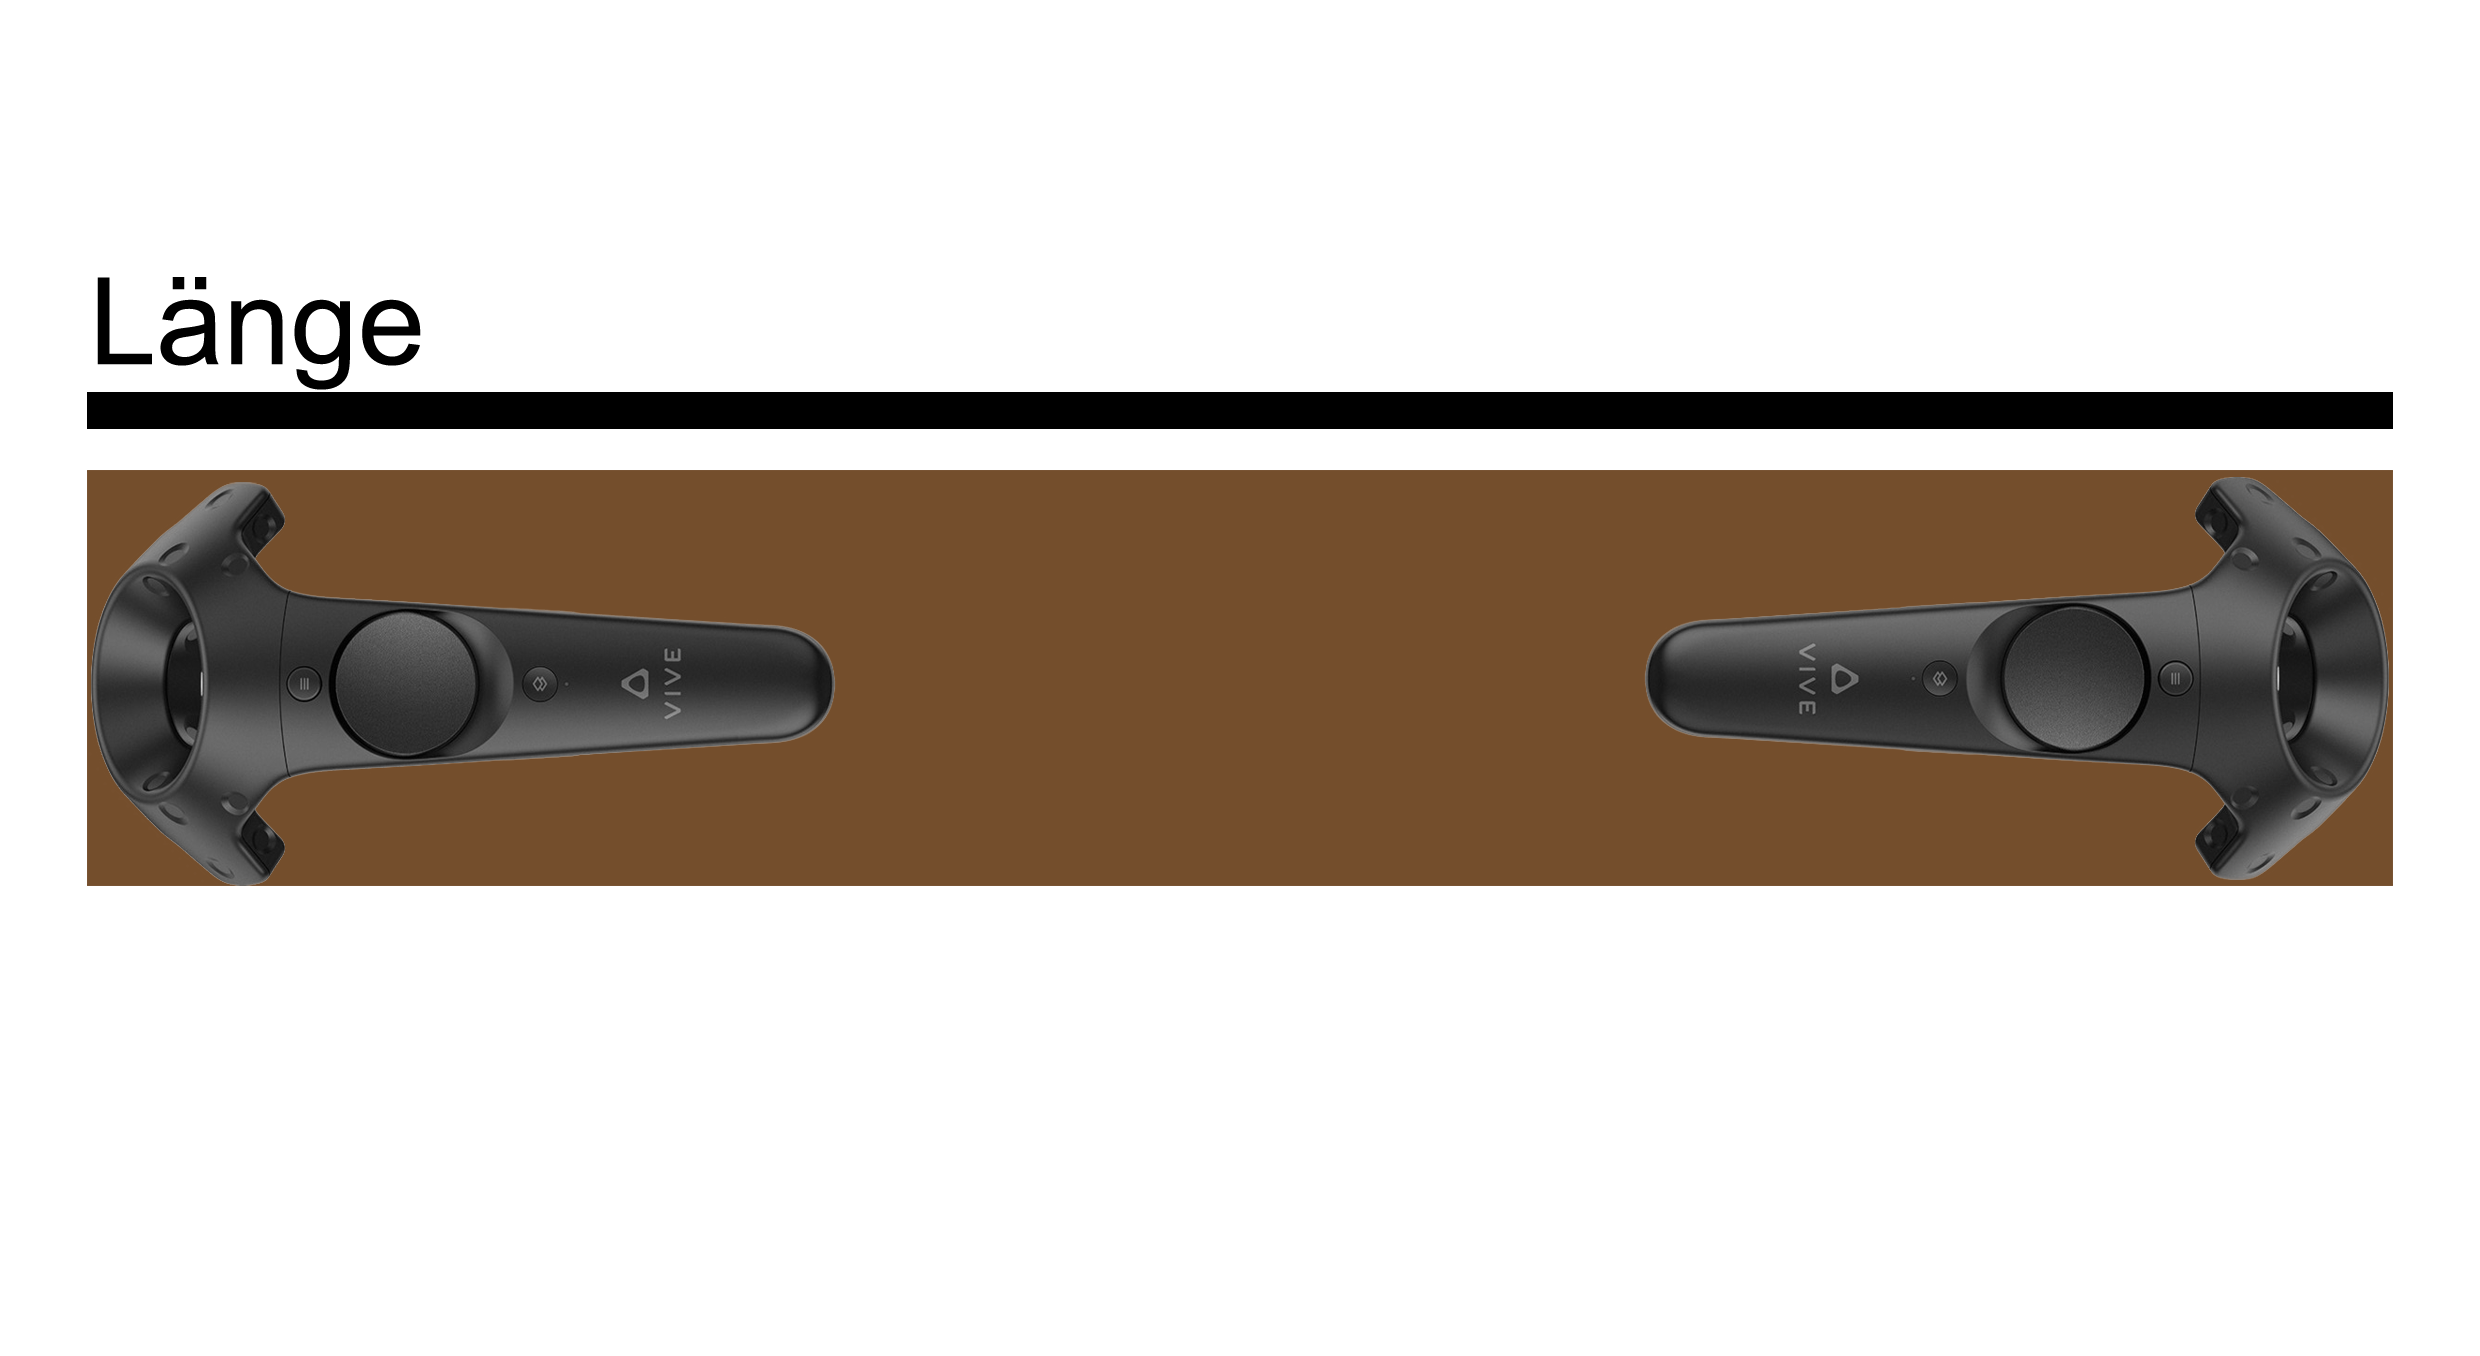
\includegraphics[scale=0.18]{pics/beam_length_measurement}
    \caption{L\"ange des Balken messen}
    \label{fig:beam_length_measurement}
\end {figure}

Dadurch weiß die Applikation wie lange der Balken ist.
Man wird aufgefordert den Trigger des Controllers zu drücken, welcher sich am Anfang des Balkens befindet, damit der Anfang und das Ende des Balkens bekannt gemacht wird.
%Grafik mit Setup Schritt 1



In Schritt zwei werden die Controller links und rechts vom Balken platziert und zeigen aufeinander.
Mit dieser Methode wird die Breite des Balkens gemessen.
%Grafik mit Setup Schritt 2
\ref{fig:beam_width_measurement} %Balken Länge Einstellen

\begin {figure}
    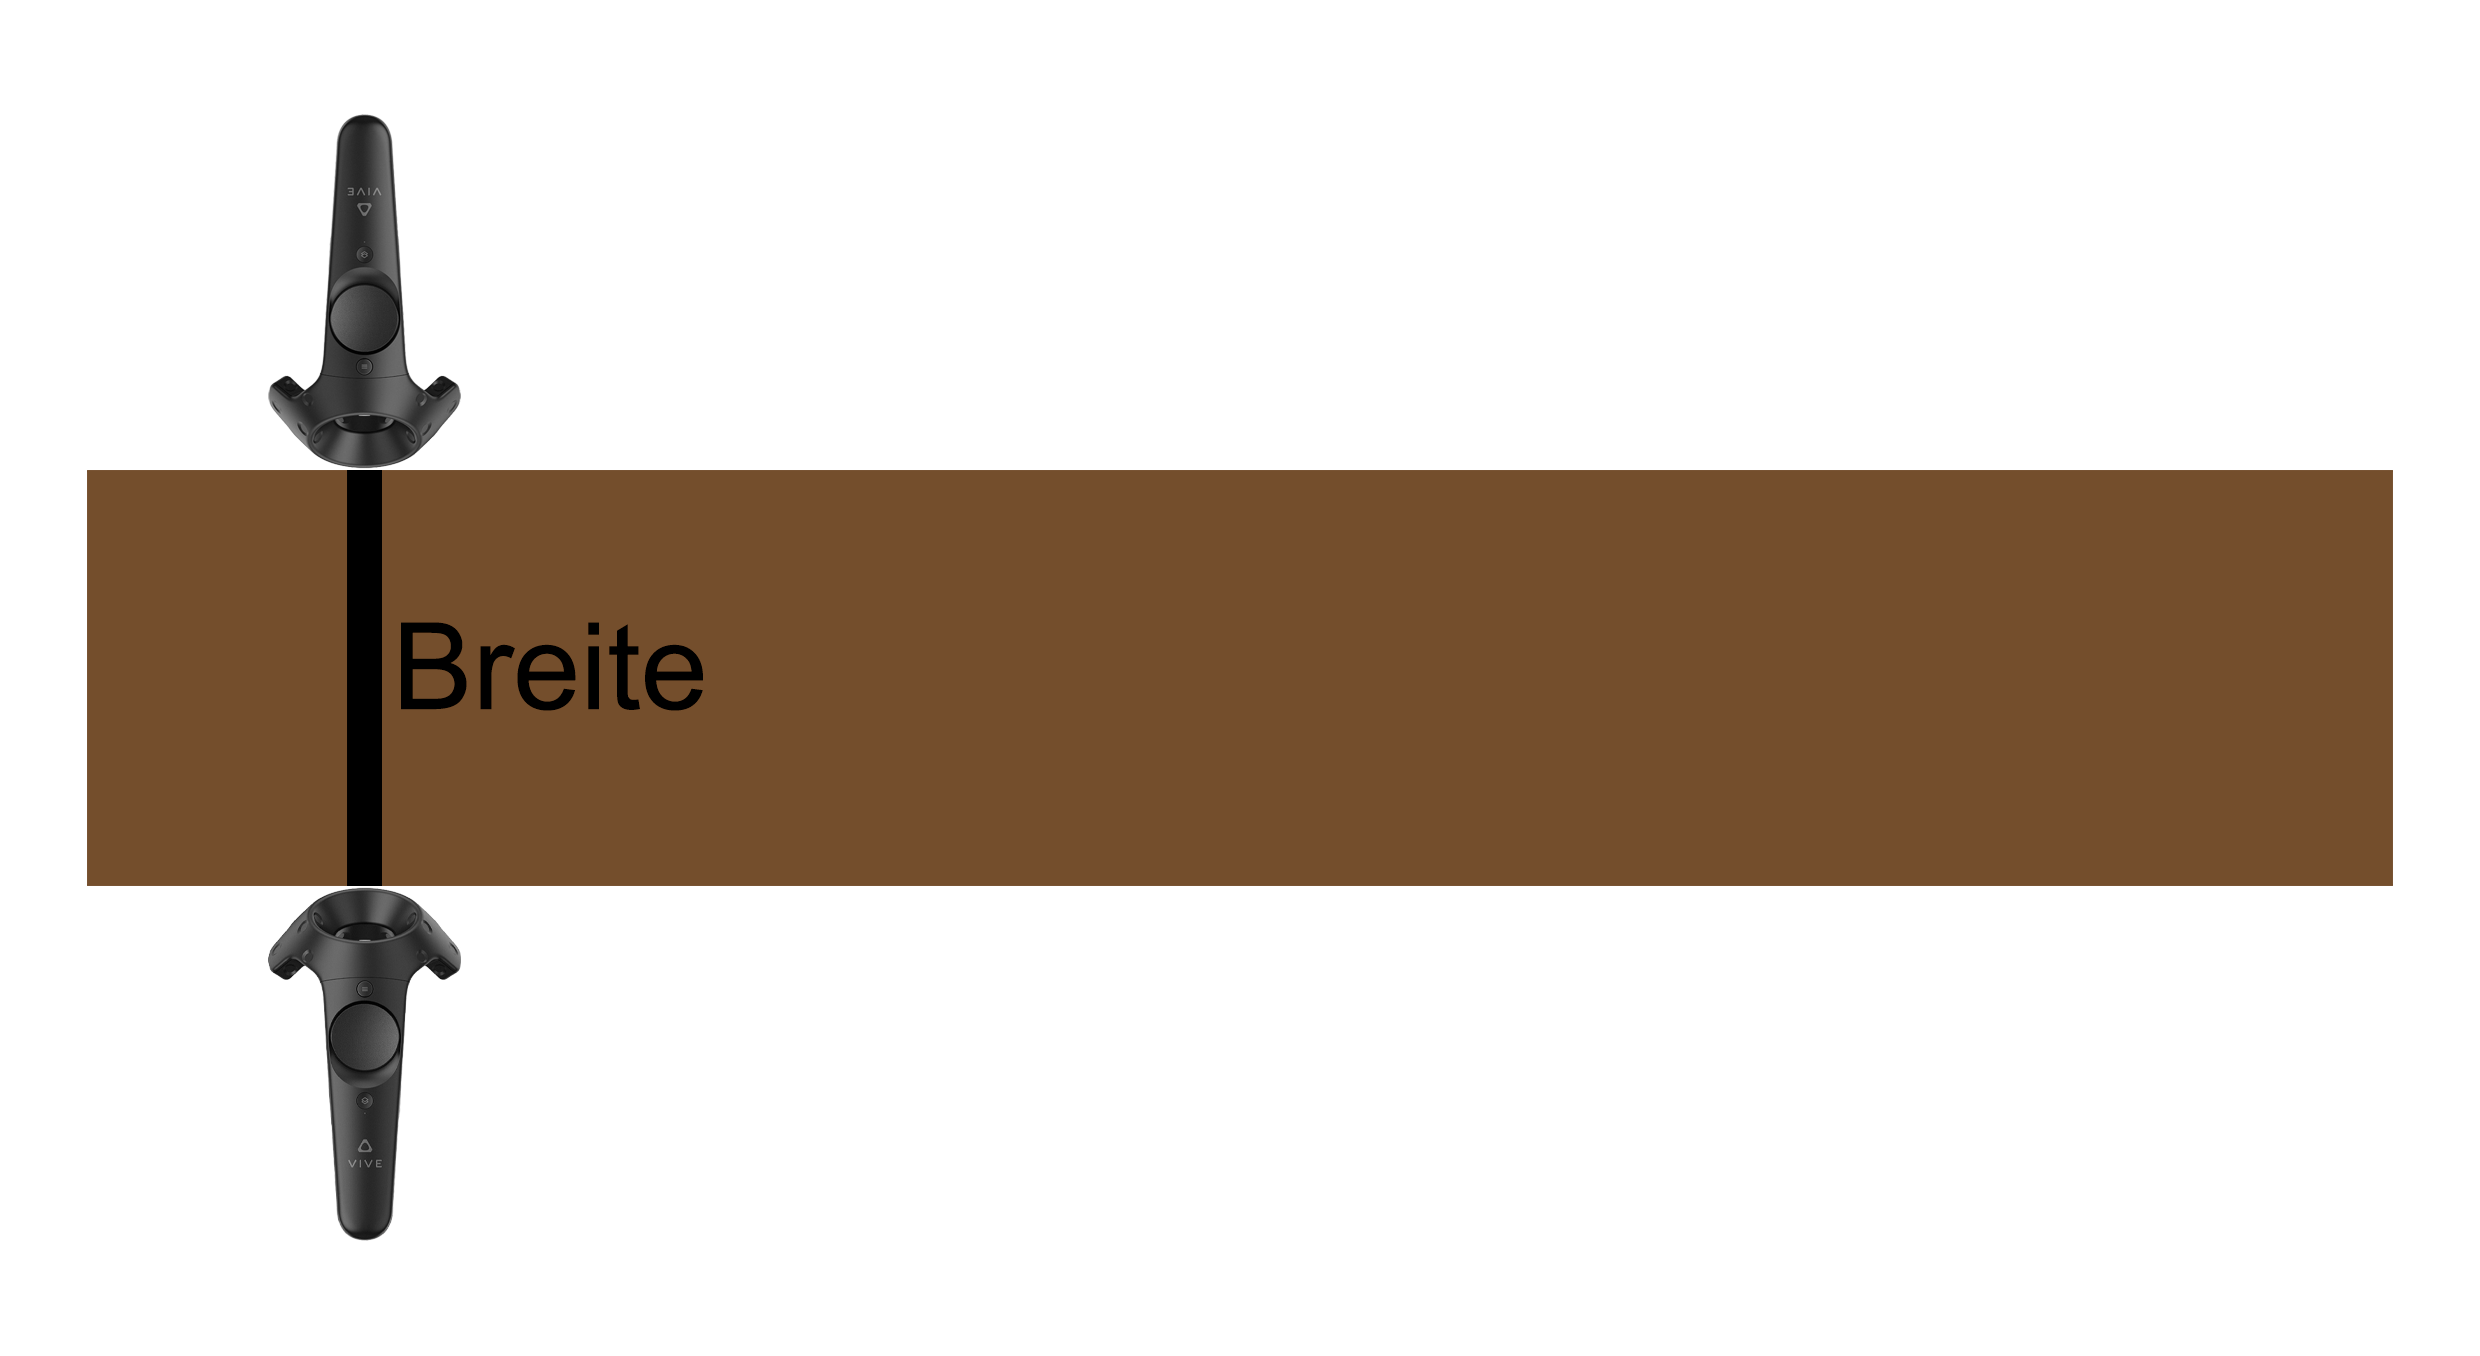
\includegraphics[scale=0.18]{pics/beam_width_measurement}
    \caption{Breite des Balken messen}
    \label{fig:beam_width_measurement}
\end {figure}


Nun ist das Setup abgeschlossen und der Balken wird richtig in der virtuellen Welt angezeigt.
~\cite{ToastGames_2021_Setup}

\subsection{Spielwelt}
\label{sec:richiesplankexperience_world}
Alle Spielmodi befinden sich in einer Stadt, welche aus einer Vielzahl an verschiedenen Gebäuden besteht.
Die Architektur ist sehr vielfältig und realistisch gehalten.
Zwischen den Bauwerken befinden sich Straßen welche mit verschiedenen Pflanzen, z.B. Bäumen, geschmückt sind.
Auf Fahrbahnen befinden sich Fahrzeuge, welche mit Schritttempo durch die Stadt fahren.

\ref{fig:richiesplankexperience_world} %Richies Plank Experience Spielwelt

\begin {figure}
    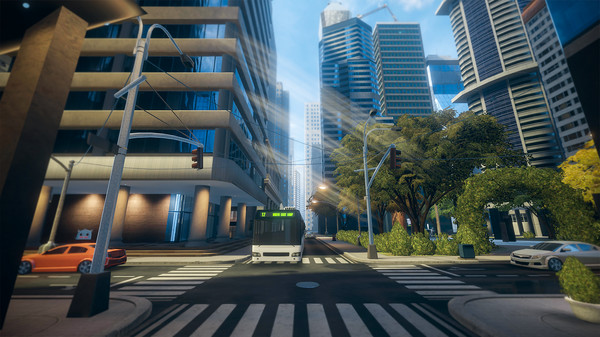
\includegraphics[scale=0.7]{pics/richiesplankexperience_world}
    \caption{Breite des Balken messen}
    \label{fig:richiesplankexperience_world}
\end {figure}


\section{VR Chat}
\label{sec:vrchat}
VR Chat befasst sich ebenfalls mit einer \"anlichen Thematik wie BeamVR.
In diesem Fall wird jedoch kein Balken sondern der ganze K\"orper des Benutzers mit Controllern getrackt.

\subsection{Spielprinzip}
\label{sec:vrchat_principle}
Wie der Name schon sagt, handelt es sich um eine in VR ausf\"uhrbare Anwendung.
Da aber nicht jeder eine VR Brille besitzt, kann man auch eine Desktop Variante spielen, welche mit Maus und Tastatur bedient wird.
In diesem Programm geht es haupts\"achlich um die Interaktion mit unbekannten Spielern aus dem Internet,
welche ebenfalls diese Applikation verwenden.
Wer jedoch mit freunden Spielen möchte, kann das nat\"urlich auch.
Eine Vielzahl an, von Spielern erstellten, Welten und Spielmodi erwarten einen und es kommen weiterhin Neue dazu.
Von einer Runde Capture the flag im Weltall, bishin zu einem entspannenden Abend an einem Lagerfeuer im Wald, ist alles möglich.
~\cite{VRChat_2021_Steam}

\subsection{Verwendungs M\"oglichkeiten}
\label{sec:vrchat_usecases}
Es gibt extrem viele m\"oglichle Verwendungszwecke für eine Applikation wie VR Chat.
Die 4 Gr\"oßten sind jedoch, die Option neue Freunde im Internet kennenzulernen, eigene Welten zu erschaffen, sein digitales Aussehen selber bestimmen zu k\"onnen und Teil einer riesigen Community zu werden.
~\cite{VRChat_2021})

VR Chat ist eine soziale Platform auf welcher sich tausende Spieler gleichzeitig befinden, diese Interagieren in Form von Gespr\"achen oder Gesten miteinander.

Die Entwickler stellen einem die n\"otigen Funktionen zur Verf\"ugung um eigene Welten zu kreiren. Die Spieler fertigen neue Spielmodi wie z.B. Capture the flag, Lasertag, Theaterauff\"uhrungen, etc. an und errichten passende Umbegungen dazu.

Wem die standard Spielermodelle nicht gefallen, kann einfach mithilfe des Steam Workshops und Tools wie Ready Player Me, Tafi oder MakeAvatar, weitere Modelle downloaden und sofort im Spiel benutzen.
Durch dieses Feature f\"uhlt sich die Applikation sofort viel pers\"önlicher an, da man sich mit den Modellen gut identifizieren kann.
~\cite{VRChat_2021_AvatarCreator}

\subsection{Full Body Tracking}
\label{sec:vrchat_fullbodytracking}
Wer die n\"otigen Tracker besitzt, hierbei handelt es sich gleich wie bei BeamVR um z.B. die Vive Tracker, kann sogar seinen K\"orper und seine Beine in dem Spiel tracken.
Dafür sind nicht mehr als 3 Schritte notwendig.
~\cite{VRChat_2021_FullBodyTracking}

Als erstes muss man in das Men\"u des Spieles gehen und auf den Kalibrieren Knopf dr\"ucken.

Als n\"achstes wird ein Spielermodell ausgew\"ahlt.
Dieses wird darauf hin in einer T-Pose vor dem Spieler ersichtlich sein.
Weiters werden mithilfe von weißen Punkten die Positionen der Tracker in der Applikation angezeit, diese Sollten nun vern\"unftig platziert werden..

Als Letztes muss man nur noch die Eingabe best\"atigt werden und das Spielermodell macht die Bewegungen des Spielers nach.

%\subsection{Avatar Erstellung}s
%\label{sec:vrchat_avatarcreation}


\begin{spacing}{1}
	\chapter{Hardware}
	\label{ch:harware}
\end{spacing}
\section{Grundlagen}
\label{sec:basics}

\subsection{Arten von VR Headsets}
\label{sec:vr-headset-types}

Bei VR Headsets werden grundsätzlich drei verschiedene Arten unterschieden:

\begin{itemize}
    \item Tethered Headsets
    \item Standalone Headsets
    \item Smartphone und Handheld Headsets
\end{itemize}

In Folge werden diese Arten kurz beschrieben, sodass die beschreibungen von der Technologien verstanden werden können.
Für eine genauere beschreibung dieses Themas wird auf~\cite{ANIWAA_TEAM_2021} verwiesen.

\emph{Tethered VR Headsets} müssen immer mit einem Computer verbunden sein, weil die VR-Applikation ausschließlich auf dem Computer läuft.
Die Brille hat dabei einerseits die Funktion die vom Computer gerenderten daten darzustellen und andererseits Positionsdaten an den Computer zurückzusenden, damit diese in der Applikationslogik verwendet werden können, um zukünftige Bilddaten zu rendern.

Bei \emph{Standalone VR Headsets} ist in der Brille ein Computer integriert, auf welchem die VR Applikation läuft.
Der Computer dient ausschließlich aus Entwicklungsplattform und die fertigen Applikationen müssen auf die Brille heruntergeladen werden.

Im Falle des \emph{Smartphone VR Headsets} läuft die Applikation auf einem Smartphone.
Um die Immersion zu erhöhen wird das Smartphone in die VR-Brille eingeschoben.
In diesem Fall dient das Telefon sowohl als Anzeigegerät als auch als Sensordatenprovider.
Die VR-Brille besteht ausschließlich aus Linsen welche die Immersion der am Handy laufenden Applikation erhöht.

\subsection{Tracking}
\label{sec:tracking}

Unter Tracking versteht man das ermitteln der Position von Objekten in der realen Welt.
Folgend werden Arten das Tracking beschrieben.
Diese beinhalten:

\begin{itemize}
    \item Outside In Tracking
    \item Markerless Inside Out Tracking
    \item Marker Based Inside Out Tracking
\end{itemize}

Wie im vorigen Abschnitt wird hier nur ein Überblick über diese Arten des Trackings gegeben.
Für nähere Informationen wird auf~\cite{Dennis_Ziesecke_2019} verwiesen.

\emph{Outside In Tracking} beschreibt das Ermitteln der Positionen durch außenstehende Sensoren.
Das bedeutet, dass das zu trackende Objekt nicht weiß wo es sich im Raum befindet (Es ist passiv).
Währenddessen ermitteln außenstehende Sensoren die Position der zu trackenden Objekte und gibt diese an die VR-Applikation weiter.

Im Gegensatz dazu gibt es das \emph{Inside Out Tracking}.
Hier ermitteln Sensoren, welche sich auf den Objekten befinden die Position derselbigen.
Dabei gibt es zwei verschiedene Arten, welche bereits oben aufgelistet worden sind.

Im Fall von \emph{Markerless Inside Out Tracking} wird natürliches Licht verwendet.
Typischerweise werden hierbei Kameras verwendet.
Die dabei aufgenommenen Bilder werden mithilfe von Bildverarbeitungsmethoden analysiert und somit wird die Position der Objekte ermittelt.

Bei \emph{Marker Based Inside Out Tracking} wird im Gegensatz kein natürliches Licht verwendet.
Hierbei ist sind die zu trackenden Objekte von Lighthouses (siehe Abschnitt~\ref{sec:lighthouse_tracking}) abhängig.
Diese beleuchten den Raum mit nicht sichtbaren licht welches von Fotosensoren an den Geräten empfangen wird.

\section{VR Headset}
\label{sec:vr-headset}
\setauthor{Quirin Ecker}

Es sind einige VR Headsets auf dem Markt.
Nach einer Statistik aus 2017 sind die beliebtesten VR Headset Hersteller Sony, Oculus und HTC (Siehe Abb.~\ref{fig:vr_headset_manufacturer_marketshare}).
Folgend sind 3 VR Brillen beschrieben.
Hierbei wurden die auf die Spielkonsolen-basierten VR Headsets nciht berücksichtigt.

\begin{figure}
    \centering
    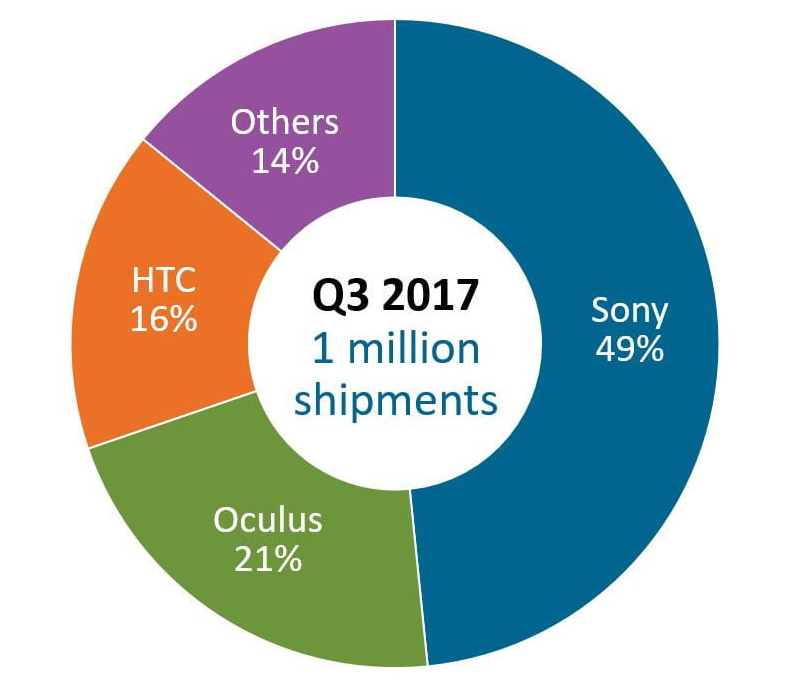
\includegraphics[scale=0.25]{pics/vr_headset_manufacturer_marketshare}
    \caption{Market-share VR Headset Hersteller~\cite{MARTINDALE_2017}}
    \label{fig:vr_headset_manufacturer_marketshare}
\end{figure}

\subsection{HTC Vive Pro}\label{sec:htc-vive}

Wie bereits in Abschnitt~\ref{sec:vr-headset-types} beschrieben, gibt es von diesen Headsets verschiedene Modelle.
Die HTC Vive Pro ist vom Typ ein tethered Headset mit dem Zusatz, dass auch sogenannte Light Houses gebraucht werden (siehe Abschnitt~\ref{sec:lighthouse_tracking}).
Andere Produkte, wie die im Folgendem beschriebene Oculus Quest benötigen solche nicht~\cite{MECHATECH}.

\subsubsection{Vorteile}

\begin{itemize}
    \item \textbf{SteamVR Verwaltung:} Die HTC kann mit SteamVR verwaltet werden, womit der manuelle Download von externer Software vermieden wird.
    \item \textbf{Lighthouse Tracking:} Zum Zeitpunkt des Verfassens dieser Arbeit ist Lighthouse Tracking verglichen mit anderen Tracking-Methoden die genaueste.
    Aus Abbildung~\ref{fig:tracking_precision_statistic} kann entnommen werden, dass das Valve Lighthouse Tracking die kleinsten Abweichungen in allen drei Dimensionen hat.
    Ein weiterer Vorteil des Lighthouse Tracking ist, dass kein natürliches Licht für den Tracking Process gebraucht wird~\cite{Dennis_Ziesecke_2019}.
    Details zum Thema Lighthouse Tracking können im Abschnitt ~\ref{sec:lighthouse_tracking} entnommen werden.
\end{itemize}

\begin{figure}
    \centering
    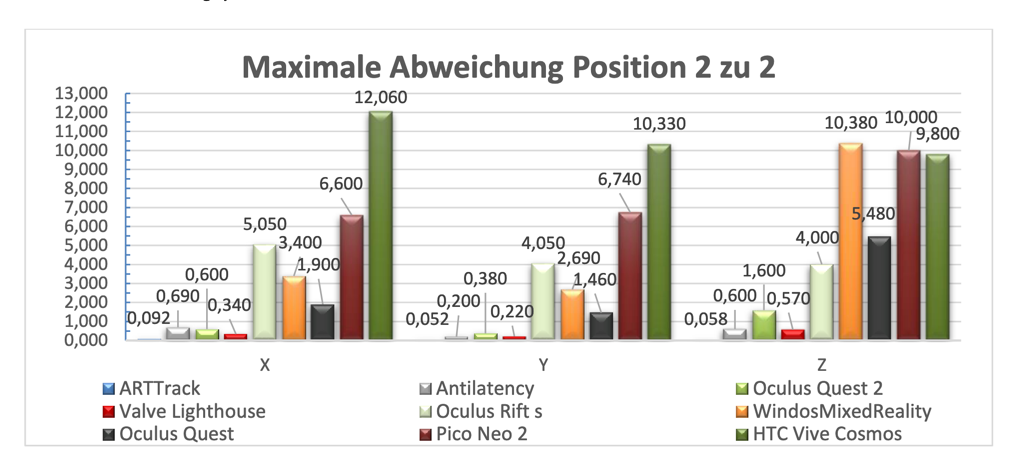
\includegraphics[scale=0.4]{pics/tracking_precision_statistic}
    \caption{Tracking Genauigkeit der VR Headsets~\cite{Macedo_2020}}
    \label{fig:tracking_precision_statistic}
\end{figure}

\subsubsection{Nachteile}

\begin{itemize}
    \item \textbf{Komplizierterer Aufbau:} Durch die Notwendigkeit der Base Stations, welche für das Lighthouse Tracking gebraucht werden, ist der Aufbau komplizierter.
    Die Base Stations müssen etwas erhöht sein, weshalb ein Stativ oder sogar eine Wandmontage notwendig ist.
    Außerdem müssen die Base Stations die zu trackenden Geräte im Sichtfeld haben.
    Für weitere Informationen wird auf den Abschnitt~\ref{sec:lighthouse_tracking} verwiesen.
    \item \textbf{Hoher Preis:} Nach der Erhebung, welche in Abb.~\ref{fig:vr_headset_prices} zu sehen ist, befindet sich die HTC Vive Pro im oberen Preissegment.
    \item \textbf{Tethered:} Wie bereits in Abschnitt~\ref{sec:basics} beschrieben worden ist, benötigen tethered Headsets eine permanente Verbindung zu einem Computer.
    Das bedeutet einerseits, dass der Transport komplizierter ist und für Normalverbraucher, ohne einen leistungsstarken Computer, der Preis für das Gesamtsystem steigt.
    Besonders der Transportaspekt ist für diese Arbeit kritisch, da diese an vielen Plätzen hergezeigt werden soll.
\end{itemize}

\begin{figure}
    \centering
    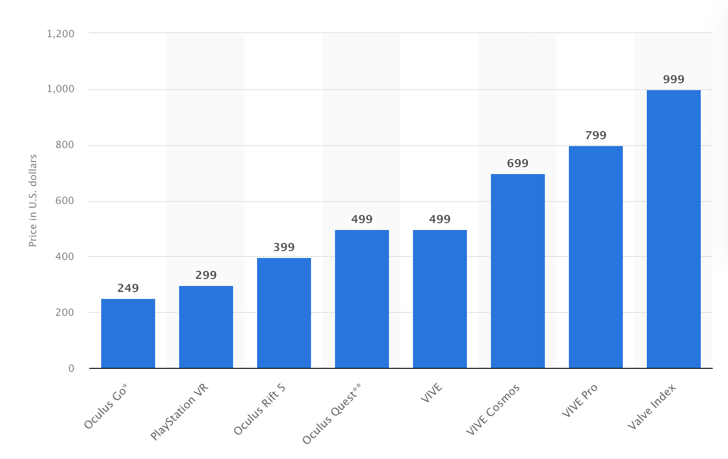
\includegraphics[scale=0.5]{pics/vr_headset_price_statistic}
    \caption{VR Headset Preise~\cite{ALSOP_2019}}
    \label{fig:vr_headset_prices}
\end{figure}

\subsection{Valve Index}

Die Valve Index ist eine VR-Brille welche von Valve entwickelt worden ist.
Diese befindet sich genauso wie die HTC Vive Pro~\ref{sec:htc-vive} im teureren Spektrum~\cite{ALSOP_2019} der VR-Brillen und ist dem Typ tethered Headset~\ref{sec:vr-headset-types} zuzuordnen.

\subsubsection{Vorteile}

\begin{itemize}
    \item \textbf{Hand Tracking}: Valve benützt bei ihren Controllern einen speziellen Entwurf.
    Die Controller besitzen eine Lasche, welche an dem Griff des Controllers hängt.
    Diese Lasche hält den Controller and der Hand, auch wenn diese den Controller nicht festhält.
    Mit dieser Technik kann der Controller losgelassen werden und die Finger frei bewegt werden.
    Um diese Finger auch in die virtuelle Welt zu übertragen, benützen die Controller Sensoren, welche an diesen angebracht sind.
    Die Informationen der Fingerpositionen können daraufhin von Entwicklern in ihren Spielen benutzt werden.~\cite{SadlyItsBradley_2019}.
    Werden diese nicht benutzt, steht trotzdem noch die normale Controller Steuerung zur Verfügung.
    \item \textbf{Lighthouse Tracking}: Die Valve Index benützt genauso wie die HTC Vive Pro das Lighthouse tracking mit dem Unterschied, dass beide Versionen des Lighthouse Tracking verwendet werden können.
    Für mehr Informationen wird auf~\ref{sec:lighthouse_tracking} verwiesen.
\end{itemize}

\subsubsection{Nachteile}

\begin{itemize}
    \item \textbf{Komplizierter Aufbau:} Genauso wie bei der HTC Vive Pro ist der Aufbau etwas komplizierter, da das Lighthouse Tracking~\ref{sec:lighthouse_tracking} verwendet wird.
    \item \textbf{Hoher Preis:} Noch teurer, wie die zuvor genannte HTC Vive Pro ist die Valve Index.
    Dies ist in der Abb.~\ref{fig:vr_headset_prices} ersichtlich.
    \item \textbf{Tethered:} Wie bereits zuvor beschrieben ist auch die Valve Index ein tethered Headset.
    Somit braucht auch diese eine permanente Verbindung zu einem Computer.
    FÜr mehr Informationen wird auf Abschnitt~\ref{sec:vr-headset-types}
\end{itemize}

\subsection{Oculus Quest 2}\label{sec:oculus-quest-2}

Die Oculus Quest 2 ist eine VR-Brille welche von Facebook/Meta im Jahre 2020 entwickelt worden is~\cite{ADI_ROBERTSON_2020}.
Diese Brille ist eine Mischung von einem tethered Headset und einem Standalone Headset~\ref{sec:vr-headset-types}.
Dies bedeutet, dass die Oculus Quest 2 ohne einen Computer benutzbar ist, aber auch mit einem USB-C Kabel zu einem Computer verbunden werden kann.
Ist das Headset mit dem Computer verbunden können PC exclusive Spiele mit der Oculus Quest 2 auch gespielt werden~\cite{ADI_ROBERTSON_2020}
Für den Aufbau werden nur das Headset und zwei Controller benötigt.

\subsubsection{Vorteile}

\begin{itemize}
    \item \textbf{Einfacher Aufbau:} Im Gegensatz zu den zuvor genannten VR-Brillen benötigt die Oculus Quest 2 kein Lighthouse Tracking verwendet.
    Dies hat einen einfacheren Aufbau zur Folge, da keine Basistationen aufgebaut werden müssen.
    Zum Aufbau werden lediglich die Brille, die Controller und eventuell noch ein Computer verwendet, wenn die Oculus Quest im tethered Modus gebraucht wird~\cite{MECHATECH}.
    \item \textbf{Günstiger Preis:} Die Oculus Quest ist im Vergleich zu den zuvor genannten Brillen eine günstigere Alternative.
    Dennoch gibt es noch günstigere VR-Headsets auf dem Markt.
    Für nähere Einsicht wird auf die Abb.~\ref{fig:vr_headset_prices} verwiesen.
    \item \textbf{Standalone:} Wie bereits beschrieben ist die Oculus Quest 2 eine Mischung aus tethered und standalone Headset.
    Kein Computer wird benötigt unter der Voraussetzung, dass auf die Leistung des Computers verzichtet werden kann.
    Für mehr Information wird auf Abschnitt~\ref{sec:vr-headset-types} verwiesen.
\end{itemize}

\subsubsection{Nachteile}

\begin{itemize}
    \item \textbf{Lichtabhängigkeit:} Durch das kamera-basierte Tracking-system~\ref{sec:oculus_quest_tracking} ist die Oculus Quest 2 von dem natürlichen Licht abhängig~\cite{Dennis_Ziesecke_2019}.
    Dieses Problem wurde von den zuvor genannten VR-Brillen durch das Licht der Basistationen gelöst~\ref{sec:lighthouse_tracking}\cite{Dennis_Ziesecke_2019}.
    \item \textbf{Full Body Tracking:} Die HTC Vive Tracker, welche üblicherweise für das Full Body Tracking verwendet werden, funktionieren mit dem Lighthouse Tracking~\ref{sec:lighthouse_tracking}.
    Da die Oculus Quest 2 diese Trackingmethode nicht verwendet kann das Full-Body-Tracking etwas komplizierter werden.
    Für verschiedene Möglichkeiten Full Body Tracking trotzdem zu erreichen wird auf~\cite{Martin_Rakver} verwiesen.
    \item \textbf{Tracking:} In Abb.~\ref{fig:tracking_precision_statistic} ist ersichtlich, dass das Tracking der Oculus Quest 2 schlechter abschneidet wie das der zuvor genannten Brillen.
\end{itemize}

\section{Lighthouse Tracking}\label{sec:lighthouse_tracking}

\subsection{Grundlagen}

Die HTC Vive Brillen und die Valve Index benützen beide das Lighthouse-Tracking~\cite{steam_lighhouse_versions}.
Diese Form des Trackings ist genauso wie das Tracking der Oculus Quest und Oculus Quest 2 (siehe~\ref{sec:oculus_quest_tracking} und~\ref{sec:oculus-quest-2}) ein Inside-Out Tracking.
Im Gegensatz zu der Oculus Quest benützt das Lighhouse Tracking kein natürliches Licht, sondern für das Auge unsichtbares Licht.
Diese Form des Tracking wird auch Marker-Based Inside-Out Tracking genannt\ref{sec:tracking}.
Im Falle des Lighhouse Tracking beleuchten die Base Stations die zu trackenden Geräte, womit sich die Geräte orientieren können.
Dies hat den Vorteil, dass die Benutzung der Vr Brille nicht von dem natürlichen abhängig ist.
Statt Kameras besitzt ein zu trackendes Gerät Fotosensoren~\cite{Buckley_2015}.

\subsection{Positionierung}

Damit dieser Vorgang fehlerfrei funktioniert werden typischerweise zwei Basestations verwendet
Diese werde wie in Abb~\ref{fig:basetstation_positioning} positioniert.
Mögliche Fehler können auftreten, wenn die Lighthouses keine klare Sicht auf die Geräte haben~\cite{steam_lighhouse_versions}..

\begin{figure}
    \centering
    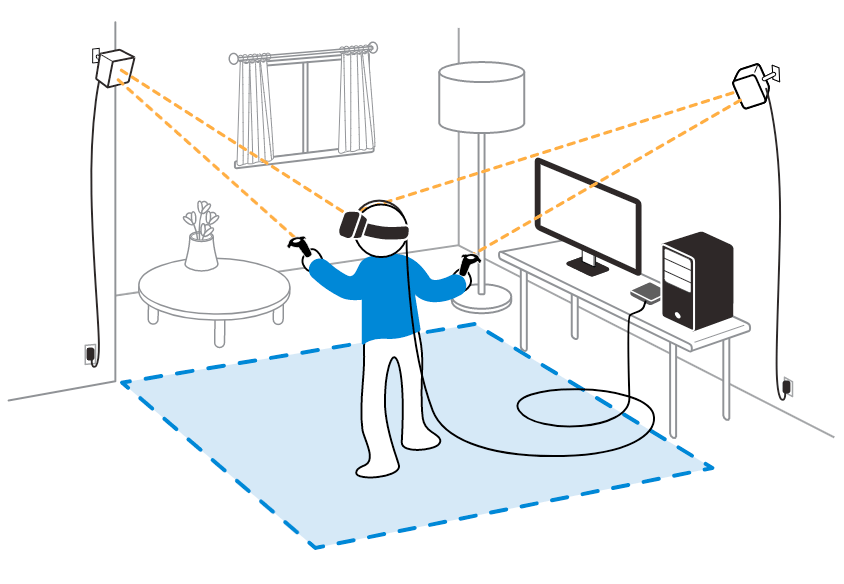
\includegraphics[scale=0.4]{pics/basestations_positioning}
    \caption{Positionierung der Lighhouses~\cite{Sercan_2018}}
    \label{fig:basetstation_positioning}
\end{figure}

\subsection{Funktionsweise}

Die Base Station besteht aus Syncblinker und Laseremitter.
Der Syncblinker ist ein Infrarot Strahl und die anderen 2 Laseremitter sind Lichtstrahlen welche sich 60-mal in der Sekunde auf einer Drehscheibe drehen.
Um die Position zu ermitteln, flasht der Sync Blinker und sobald dieser bei der Brille ankommt, fängt das Gerät zu zählen an bis die Lichtstrahlen der Laseremitter ankommen.
Durch die Drehscheibe, auf der sich die Laseremitter befinden, beleuchtet die Base Station so viele wie mögliche Sensoren.
Die Position mehrerer Punkte des Gerätes ist somit bekannt und es kann die Rotation der Brille ebenfalls berechntet werden~\cite{Buckley_2015, Skarredghost_2017}.

\subsection{Versionen}

Zum Zeitpunkt das Verfassen der Diplomarbeit gibt es 2 Versionen der Base Stations.
Version 1.0 und 2.0 sind nicht miteinander kompatibel.
Folgend sind die Versionen aufgelistet mit den jeweils kompatiblen Geräten in der Klammer.
Wobei Steam bei der Kompatibilität nur HTC Brillen und die Valve Index vermerkt haben, weshalb andere Brillen in der folgenden Liste ausgenommen worden sind~\cite{steam_lighhouse_versions}.

\begin{itemize}
    \item Lighthouse 1.0 (HTC Vive, Valve Index)
    \item Lighthouse 2.0 (HTC Vive Pro, Valve Index)
\end{itemize}

\emph{1.0 Lighthouses} besitzen eine nahezu quadratische form mit einer Länge von 15 cm, einer Breite von 16 cm und einer höhe von 10 cm

\emph{2.0 Lighthouses} haben einer eher rechteckige form mit einer Länge von 15 cm, einer Breite von 13,30 cm und einer Höhe von 12,90 cm.
Die Vorderseite ist der Länge nach abgerundet, mit welcher eine höhere Reichweite erreichbar is.
Mit der neuen Version ist es auch möglich mehrere Base Stations zu verwenden.
Durch die erhöhte Sichtweite und der Möglichkeit mehr wie zwei Lighthouses zu verwenden kann eine größere Spielfläche verwendet werden.
Der Sichtkontakt der Lighhouses ist nicht mehr nötig~\cite{Cale_2019}.

\section{Oculus Quest Tracking}
\label{sec:oculus_quest_tracking}

Eine weitere Art das Tracking wird benutzt von Oculus.
Wie bereits in~\ref{sec:lighthouse_tracking} erwähnt benutzt die Oculus Quest und Oculus Quest 2 ein Inside Out Tracking.
Die Oculus Quest benützt Kameras, um sich im VR Raum zu orientieren.

\subsection{DoF}

Es gibt zwei verschiedene Arten des Oculus Quest und Oculus Quest 2 Tracking zwischen denen das Headset wechseln kann.
Diese arten gelten nur für das VR Headset und nicht die Controller~\cite{oculus_support_headset_tracking}.

\begin{itemize}
    \item 3DoF
    \item 6Dof
\end{itemize}

\emph{3DoF} bedeutet, dass die Rotation des VR Headsets getracked werden.
Die Position wird nicht getracked.
Oculus empfehlt nur im Sitzen oder im Stehen zu spielen, wenn 3DoF aktiviert ist.

Bei \emph{6DoF} wird auch die Position getracked.
Viele Spiele setzen vorraus, dass die Position getracked wird.

\subsection{Headset Tracking}

Das Oculus Quest 2 Headset benützt ein etwas anderes Tracking.
Durch die Kameras, welche in dem Headset verbaut, sind analysiert es die Umgebung.
Mit Bildverarbeitung erstellt es es aus den aufgenommenen Bildern eine 3d Map.
Diese 3d Map wird benutzt um das Headset im dreidimensionalen Raum zu positionieren und rotieren~\cite{MECHATECH}.

\subsection{Controller Tracking}

Oculus nennt ihre virtual reality controller oculus touch.
Diese haben einen ring welcher einen Ring um die Hand Bilden, auf welchen sich eine Infrarot LED befindet.
Die Infrarot LED ist so positioniert, damit sie in die Richtung des Headsets schauen.
Parallel machen die Kameras, welche auf dem Headset sich befinden, Fotos.
Durch die Infrarot LED Strahlen kann das Headset mit den Fotos die Position der Controller ermitteln.
Das Infrarotlicht der Controller ist für das menschliche Aug nicht sichtbar~\cite{Gajsek_2022}.
Im Gegensatz zum Headsets benützen die Controller nach definition ein Outside in Tracking, da die Controller nicht von alleine wissen, wo sie sich im Raum befinden und das tracking mithilfe des Headset funktioniert.

\subsection{Guardian}

Oculus Guardian ist ein Sicherheitssystem, bei welchen man eine gewisse Spielfläche definieren kann.
Die Grenzen der Spielfläche werden dann angezeigt, wenn man sich diesen nähert~\cite{Oculus_Guardien}.

\emph{Guardian Space Sense} ist ein weiteres Sicherheitssystem.
Durch die 3d Map, welche schon in dem Abschnitt Headset Tracking beschrieben worden ist, kann auch eine Hilfestelle für den Nutzer geleistet werden.
Hier versuch die Oculus Quest Umrisse von Gegenständen, Menschen und anderen Lebewesen in der virtuellen realität sichtbar zu machen, wenn sich der Nutzer diesen nähert~\cite{Oculus_Guardien}.

\section{Wireless Virtual Reality}
\label{subsec:wireless-virtual-reality}

VR-Brillen wie die HTC Vive, HTC Vive Pro, Valve Index und zu einem bestimmten Ausmaß auch die Oculus Quest 2 hängen normalerweise and einem Kabel.
Diese Brillen werden auch tethered Headsets genannt und wurden bereits in dieser Arbeit in dem Abschnitt~\ref{sec:vr-headset-types} beschrieben.
Durch die permanente Anbindung an einen Computer kann das Kabel die Mobilität einschränken und die Immersion brechen~\cite{Oculus_2021}.
Aus diesem Grund gibt es einige Lösungen, die dieses Problem lösen wollen.
Folgend werden zwei Lösungen näher Erläutert.
Diese umfassen den Oculus Air Link und Vive WLAN Adapter.

\subsection{Vive Wireless Adapter}

Bei dem Vive wireless Adapter wird zusätzliche Hardware zur Brille benötigt.
Diese beinhalten:

\begin{itemize}
    \item Powerbank
    \item Wireless Link Box
    \item PCIe WiGig Card
    \item anderes Zubehör
\end{itemize}

Für Informationen zu der zusätzlichen Hardware wird auf~\cite{ViveWirelessAdapter} verwiesen

Zum Zeitpunkt der Erstellung dieser Arbeit konnten keine zuverlässigen technischen Spezifikationen gefunden werden.
Daher kann die Funktionsweise nur sehr oberflächlich beschrieben werden.

Grundsätzlich wird für die Funktionalität die Wireless Link Box gebraucht, welche mit der PCIe WiGig Card verbunden ist.
Die Wireless Link Box kombiniert mit der Antenne welche sich auf der VR-Brille befindet verschafft HTC ein möglichst latenz freies Erlebnis.
Durch die ständige Bewegung der VR-Brille variiert die Brandweite konstant.
Für dieses Problem benützt der Wireless Adapter einen Algorithmus welcher das Videosignal je nach Bandbreite in echtzeit komprimiert~\cite{VRConduit_2018}.

Durch die zusätzliche Hardware ist die HTC Lösung etwas teuer.
Eine Lösung ohne zusätzliche Kosten wurde von Oculus entwickelt und wird Oculus Air Link genannt.

\subsection{Oculus Air Link}

Auch, wenn die Oculus Quest 2 und Oculus Quest bereits wireless Headsets sind kann man diese wie bereits zuvor beschrieben mit dem Computer verbinden.
Diese Verbindung wird Oculus Link genannt und besteht aus einem qualitativ hochwertigen USB C 3.0 Kabel~\cite{William_2020}.

Um die Leistung eines PCs nun in Anspruch zu nehmen, ohne das Kabellose Erlebnis aufzugeben, entwickelte Oculus Quest Oculus Air Link~\cite{Oculus_2021}.
Oculus Air Link wurde mit der Version 28 zu der Oculus Quest 2 hinzugefügt, welche am 19\. April 2021 herausgekommen ist~\cite{Oculus_2021, oculus_patchnotes}.

Der Oculus Air Link braucht im Gegensatz zu dem zuvor genannten Vive Wireless Adapter keine weitere Hardware um zu funktionieren.
Um diesen zum Laufen zu bekommen wird nur die Oculus App gebraucht.
Einer der Gründe dafür ist, dass kein zusätzlicher Akku für die Brille notwendig ist, da dieser sowieso schon für das standalone Erlebnis gebraucht wird.
Für mehr Informationen zu dem Aufsetzen des Oculus Air Link wird auf~\cite{Oculus_AirLink} verwiesen.

Ähnlich wie der Vive Wireless Adapter benützt der Oculus Air link auch WLAN für die Datenübertragung~\cite{Oculus_2021}.
Dabei benützt Oculus die gleiche Streaming-Pipeline welche auch bei Oculus Link verwendet worden ist~\cite{Oculus_2021}.


\begin{spacing}{1}
	\chapter{Software}
	\label{ch:software}
\end{spacing}
\section{Game Engine}\label{sec:game-engine}

Es gibt mehrere Games Engines mit welchen eine VR Applikation entwickelt werden kann.
In Abb.~\ref{fig:game_engine_marketshare} ist der Marktanteil verschiedener Engines abgebildet.
Diese Daten sind aber mit Vorsicht zu genießen, da das Skript welche diese Daten geliefert hat nach einigen Kriterien handelt,(siehe~\cite{REDDIT_2018}).
Dies bedeutet beispielsweise, dass nur Spiele mit einer Wikipedia Seite mit einberechnet werden.

\begin{figure}
    \centering
    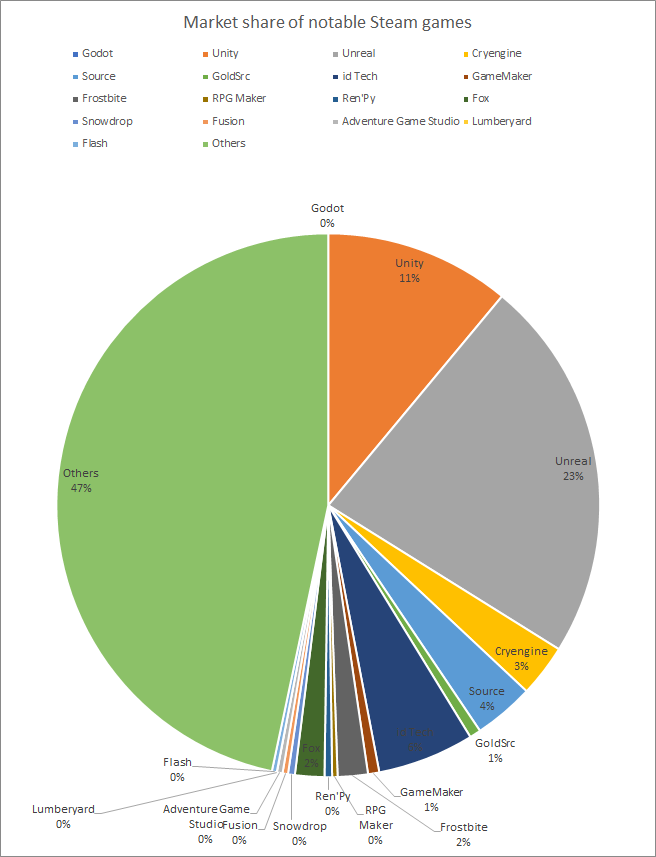
\includegraphics[scale=0.4]{pics/game_engine_marketshare}
    \caption{Game Engine Market-share~\cite{REDDIT_2018}}
    \label{fig:game_engine_marketshare}
\end{figure}

\begin{figure}
    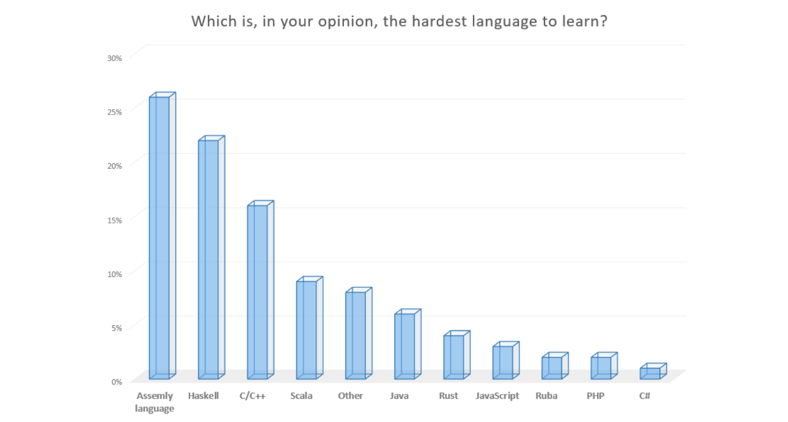
\includegraphics[scale=0.4]{pics/programming_languages_hardest}
    \caption{Schwerste Programmiersprachen~\cite{JAXCENTER_2018}}
    \label{fig:hardest_programming_languages}
\end{figure}

\subsection{Unity}\label{subsec:unity}

Unity ist eine Game Engine, welche von Unity Technologies initial exklusiv für Apple Mac OS X entwickelt wurde.
Die Engine wurde portiert und kann heute auch auf Windows und auf der Linux Plattform benützt werden.
Sie ist für alle im prinzip gratis bis zu einem bestimmten Umsatz.
Auch wenn sie eine Einsteiger Engine genannt wird, ist sie trotzdem im professionellen Bereich in benutzung und viele bekannte Spiele, wie Pokemon GO, Among us und Hearthstone wurden in der Unity Engine entwickelt~\cite{Haas2014AHO,Unity_System_Specification,UNITY_PRICING_1,WIKIPEDIA_UNITY_GAME_LIST_2014}.

\subsubsection{Vorteile}\label{subsubsec:vorteile}

\begin{figure}
    \centering
    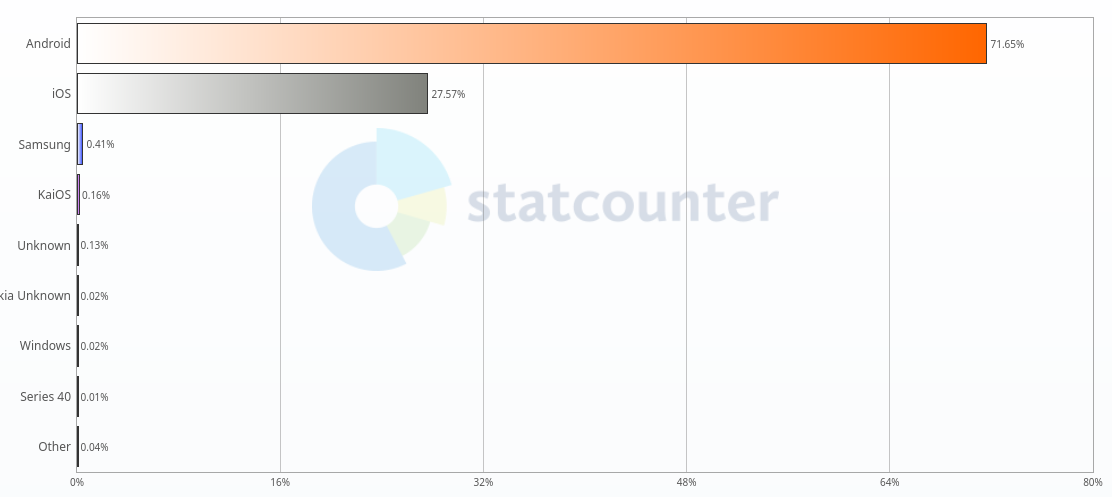
\includegraphics[scale=0.35]{pics/mobile_os_marketshare}
    \caption{Mobile Betriebssystem Market Share~\cite{StatCounter_Mobile_2021}}
    \label{fig:mobile-os-market-share}
\end{figure}

\begin{figure}
    \centering
    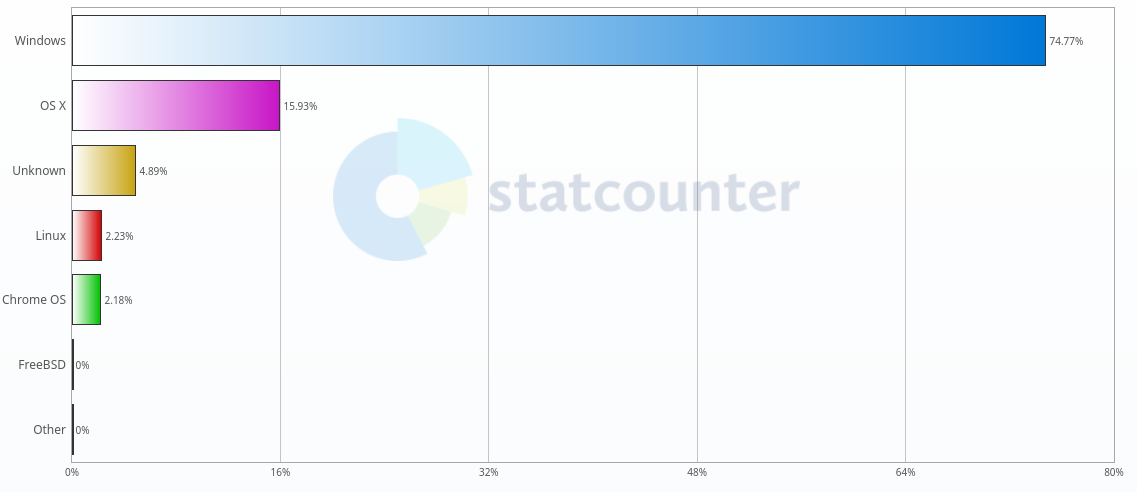
\includegraphics[scale=0.35]{pics/desktop_os_market_share}
    \caption{Desktop Betriebsystem Market Share~\cite{StatCounter_Desktop_2021}}
    \label{fig:desktop-os-market-share}
\end{figure}



\begin{itemize}
    \item \textbf{Leichter Einstieg:} Das Einsteigen in Unity ist ein sehr einfacher Prozess.
    Die einzige Voraussetzung für den Start einer Unity Applikation ist ein Unity Account.
    Nach der Erstellung eines Accounts kann das Unity Hub heruntergeladen werden.
    Anschließend kann in dem Unity Hub eine Version der Unity Engine heruntergeladen werden~\cite{Unity_Download}.
    Anfangs ist die Engine gratis, fallen nach einem bestimmten Umsatz an~\cite{Unity_Pricing_2}.
    \item \textbf{Programmiersprache:} In Abb.~\ref{fig:hardest_programming_languages} ist ersichtlich, dass viele Programmierer der Meinung sind, C\# einer der einfacheren zu lernenden Sprachen ist.
    Verglichen mit den C++, welches die Programmiersprache der Unreal Engine ist, hat sie nach der Abb. eine weitaus kleinere Lernkurve.
    \item \textbf{Plattform Kompatibilität:} Applikationen, welche in Unity entwickelt worden sind haben eine hohe Plattformunabhängigkeit.
    Unity Applikationen können für die größten Desktop- und Mobile Betriebssysteme gebaut werden.
    Siehe dazu Abb.~\ref{fig:desktop-os-market-share} und Abb.~\ref{fig:mobile-os-market-share}.
    Für eine volle Liste der unterstützten Plattformen wird auf~\cite{UNITY_PLATTFORMS} verwiesen.
\end{itemize}

\subsubsection{Nachteile}

\begin{itemize}
    \item \textbf{Market Share:} Nach Abb.~\ref{fig:game_engine_marketshare} hat die Unity Engine weniger Market-share wie beispielsweise die Unreal Engine.
    \item \textbf{Kostenanfall:} Es ist in~\cite{UNREAL_ENGINE_PRICING_2022} und~\cite{Unity_Pricing_2} ersichtlich, dass bei Unity schneller Kosten anfallen wie bei der Unereal Engine.
    Das bedeutet nicht, dass die Kosten bei Unity mehr sind wie bei Unreal Engine, sondern, dass die kostenlose Entwicklungsphase bei Unreal länger ist.
\end{itemize}

\subsection{Unreal Engine}
\label{subsec:unreal_engine}

Unreal Engine wird von Epic Games entwickelt~\cite{UNEAL_ENGINE_OWNER_2022}.
Diese Engine ist eine weit verbreitete Game Engine.
Dies kann man Abbildung~\ref{fig:game_engine_marketshare} entnehmen.
Viele Spiele wie Fortnite, Ark Survival Evolved, Borderlands 3 und Jedi Fallen Order sind mit dieser Engine entwickelt worden~\cite{WIKIPEDIA_UNREAL_GAME_LIST}.

\begin{figure}
    \centering
    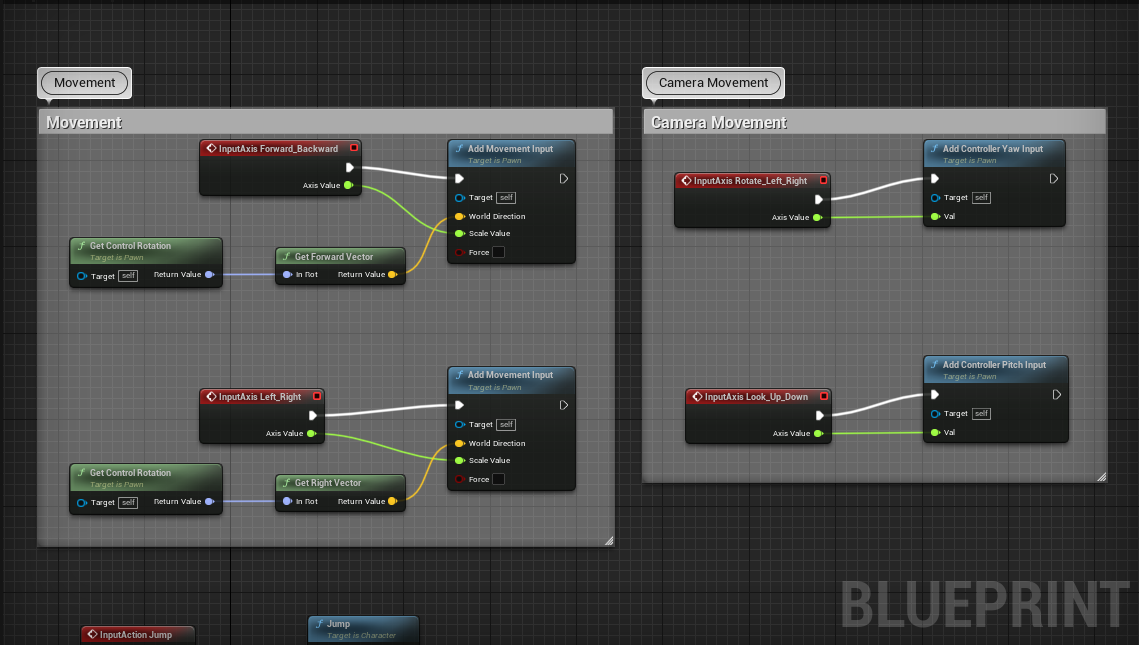
\includegraphics[scale=0.3]{pics/visual_scripting_unreal_engine}
    \caption{Visual Scripting in Unreal Engine 5}
    \label{fig:visual_scripting_unreal_engine}
\end{figure}

\subsubsection{Vorteile}

\begin{itemize}
    \item \textbf{Market Share:} In Abb.~\ref{fig:game_engine_marketshare} ist ersichtlich, dass Unreal den Größten Market Share.
    Dies ist genauso wie zuvor mit Vorsicht zu genießen, da diese Daten wie bereits beschrieben unter einem bestimmten Kriterium gesammelt worden sind.
    \item \textbf{Visual Scripting:} Unreal Engine benutzt für das Scripting der Applikation neben der Programmiersprache C++ ein visual scripting System, welches auch Blueprint genannt wird.
    Anders wie in Bolt, welches das Visual Scripting Tool für Unity ist, ist das Blueprint System bereits eingebaut.
    Bolt muss noch extra installiert und konfiguriert werden~\cite{Unity_Bolt}.
    Das integrierte Blueprint System hat seine Nachteile und seine Vorteile.
    Ein Vorteil ist die abgeschwächte Lernkurve, die das System gegenüber von C++ bietet um die Unreal Engine kennenzulernen.
    Dies zumindest nach~\cite{Mower_UnrealEngine} und~\cite{jwatte_2017}.
    ~\ref{fig:visual_scripting_unreal_engine}
    \item \textbf{Kostenanfall:} Wie bereits bei den Nachteilen der Unity Engine besprochen fallen die Kosten bei der Unreal Engine langsamer and wie bei der Unity Engine..\cite{UNREAL_ENGINE_PRICING_2022, Unity_Pricing_2}
\end{itemize}

\subsubsection{Nachteile}

\begin{itemize}
    \item \textbf{Unterstützte Spielplattformen:} Applikationen, welche mit Unreal Engine gemacht worden sind können für weniger Plattformen entwickelt werden wie bei der Unity Engine~\cite{Viscirele_Unreal_v_Unity}.
    \item \textbf{Unterstützte Entwicklerplattformen:} Mit der Unreal Engine ist es möglich auf den drei größten Desktop Betriebssystemen, welche in Abb.~\ref{fig:desktop-os-market-share} ersichtlich sind, zu entwickeln.
    Dennoch ist es komplizierter die Game Engine auf Linux zu installieren, da man hier die Game Engine selber von der Quelle bauen muss.
    Es gibt keinen offiziellen Binary Installer für Linux~\cite{Unreal_Installationsguide}.
    \item \textbf{C++:} Für erweiterte Funktionalität, welche nicht mit dem Blueprint System implementiert, werden kann, muss auf C++ zurückgegriffen werden.
    In Abb.~\ref{fig:hardest_programming_languages} ist zu sehen, dass C++ eine starke Lernkurve hat.
\end{itemize}

\subsection{Source Engine und Source 2 Engine}
\label{subsec:source-engine-und-source-2-engine}

Es gibt mittlerweile 2 Iterationen dieser Engine.
Zum einen die originale Source Engine und die Source Engine 2.
Die Markteinführung der ursprünglichen Source Engine war im Juni 2004~\cite{Bryan_Wirtz_SOURCE_ENGINE_2022}.
Daraufhin ist die Source 2 Engine im August 2014 erschienen~\cite{VALVE_DEVELOPER_COMMUNITY_SOURCE2}.
Beide Engines sind von Valve entwickelt worden~\cite{VALVE_DEVELOPER_COMMUNITY_SOURCE, VALVE_DEVELOPER_COMMUNITY_SOURCE2}.
Verantwortlich ist die Source 2 Engine für Spiele wie Dota 2 und Half Life Alyx~\cite{WIKIPEDIA_SOURCE2_ENGINE_GAME_LIST}.
Andere Spiele wie Half Life 2, Counterstrike Source, Portal, Portal 2 und Counterstrike Global Offensive sind mit der originalen Source Engine entwickelt worden~\cite{WIKIPEDIA_SOURCE_ENGINE_GAME_LIST}.
Auch als VR Entwicklungsumgebung eignet sich die Source 2 Engine, da sie für Half Life: Alyx, eines der erfolgreichsten VR Spiele benutzt worden ist~\cite{WIKIPEDIA_SOURCE2_ENGINE_GAME_LIST, Aden_Carter_2020}.
Die folgenden Vorteile und Nachteile beziehen sich auf die Source 2 Engine.

\subsubsection{Vorteile}

\begin{itemize}
    \item \textbf{Gratis:} Die Source Egnine ist grundsätzlich komplett Gratis.
    Es gibt keine Kostenanfälle durch das nutzen der Engine.
    Das einzige Kriterium von Valve ist, dass die Engine auf Steam publiziert werden muss~\cite{Brenna_Hillier_2015}.
\end{itemize}


\subsubsection{Nachteile}\label{pgr:cons}

\begin{itemize}
    \item \textbf{Market Share:} In Abb.~\ref{fig:game_engine_marketshare} ist ersichtlich, dass die Source Engine verglichen mit den zuvor gennanten Game Engines keinen großen Marktanteil hat.
    Weniger Nutzung einer Engine bedeutet auch weniger unterstützung, welche es online zur Verfügung gibt.
    \item \textbf{Publizierung:} Wie bereits bei den Vorteilen angesprochen, muss ein Spiel, welches mit der Source Engine entwickelt worden ist auch auf Steam publiziert werden~\cite{Brenna_Hillier_2015}.
\end{itemize}

\section{VR in Unity}\label{sec:vr-in-unity}
\setauthor{Florian Beckerle}
Unity bietet bereits eine eingebaute Basis VR API, welche ein paar Features für die Verwendung von VR Geräten zur Verfügung stellt.
Diese muss jedoch erst eingstellt werden, das geht in folgenden Schritten.

Um VR für die Spiele zu aktivieren, müssen zuerst die Player Settings, welche im Menü bei Edit > Project Settings > Player zu finden sind, geöffnet werden.
Als nächstes muss die Option Virtual Reality Supported aktiviert werden, sodass in der Box ein Haken zu erkennen ist, siehe Abb. ~\ref{fig:unity_vr_api_settings}.
In der darunter stehenden Liste, namens Virtual Reality SDKs, kann nun mit dem Plus-Knopf eine neue SDK hinzugefügt werden.
Ein Beispiel hierfür wäre die Oculus SDK.
Der Minus-Knopf bietet die Möglichkeit, diese SDKs wieder zu entfernen, siehe Abb. ~\ref{fig:unity_vr_api_settings}.
~\cite{Unity_VR_Overview_2022}

Wenn VR aktiviert wurde, wird das Spiel automatisch auf die VR-Brille gerendert und dort angezeigt.
Weiters besitzt jede Kamera, welche im Spiel ist, eine Option, auf welches Auge das Ausgangssignal angezeigt werden soll, zum Beispiel linkes-, rechtes-, beide- oder keine Augen.
Unter den Augen versteht man die Bildschirme der VR-Brille welche sich vor den Augen des Benutzers befinden.
Ein weiteres automatisches Feature ist, dass die Bewegung der VR-Brille, in der Realtität auf die Position der Kamera im Spiel übertragen wird.

Unity empfiehlt für die Verwendung der Api folgende Brillen: Gear VR, Oculus CV1 und die Vive.
~\cite{Unity_VR_Overview_2022}

\begin {figure}
    \centering
    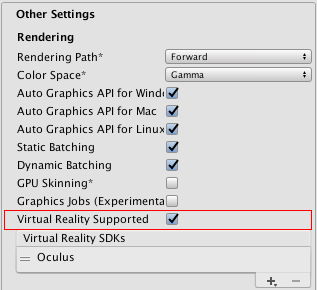
\includegraphics[scale=0.8]{pics/unity_basis_vr_api_settings}
    \caption{Unity VR API - Settings}
    \label{fig:unity_vr_api_settings}
\end {figure}

\section{VR Plugin}\label{sec:vr-plugin}
\setauthor{Florian Beckerle}
Für BeamVR wurde das SteamVR Unity Plugin verwendet.
Es wurde von Valve entwickelt und bietet bereits eine Vielzahl an vorgefertigten Demos, welche mit der Installation des Plugins mitgeliefert werden, diese werden später genauer beschrieben.
~\cite{SteamVR_Overview_2022}

\subsection{Quickstart}\label{subsec:quickstart}
\setauthor{Florian Beckerle}
Für das Setup des SteamVR Unity Plugins sind 5 Schritte notwendig.
Damit alles funktioniert muss SteamVR von Steam und das Plugin vom Unity Asset Store gedownloaded werden.
Nachdem die Installation beider Softwares abgeschlossen wurde, muss das Plugin über den Package Manager in das Unity Projekt importiert werden.
Im Menu Window wird nun eine neue Option namens SteamVR Input angezeigt, siehe Abb. ~\ref{fig:steamvr_input_menu_item}.
\begin {figure}
    \centering
    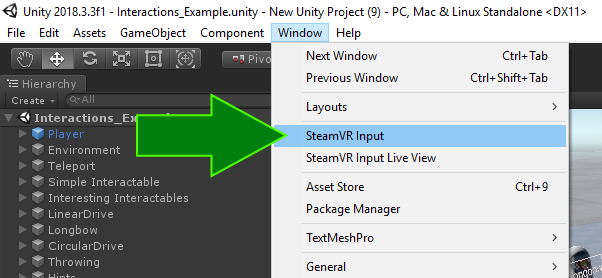
\includegraphics[scale=0.9]{pics/steamVR_Input_MenuItem}
    \caption{Steam VR - Input Menu Item}
    \label{fig:steamvr_input_menu_item}
\end {figure}
Wenn man auf diese klickt, erscheint ein Popup, welches fragt, ob JSON Files kopiert werden sollen, dort drückt man auf Ja, siehe Abb. ~\ref{fig:steamvr_copy_json}.
\begin {figure}
    \centering
    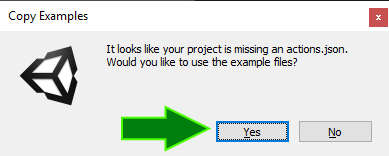
\includegraphics[scale=1]{pics/steamVR_Input_CopyJSON}
    \caption{Steam VR - Copy JSON}
    \label{fig:steamvr_copy_json}
\end {figure}
Nachdem der Vorgang abgeschlossen ist, öffnet sich das SteamVR Input Fenster, dort muss nun Save and Generate gedrückt werden, siehe Abb. ~\ref{fig:steamvr_save_and_generate}.
\begin {figure}
    \centering
    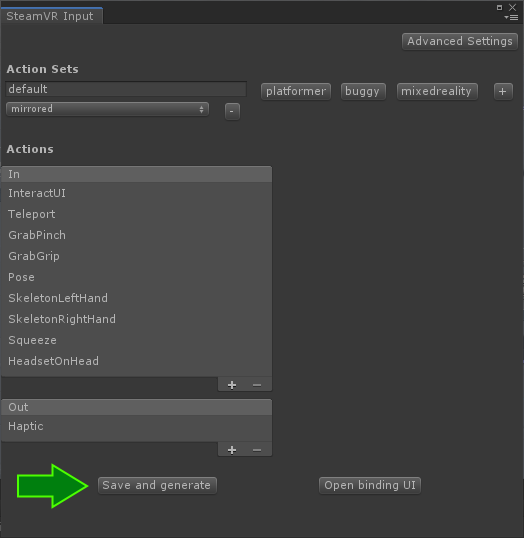
\includegraphics[scale=0.6]{pics/steamVR-Input-SaveAndGenerate}
    \caption{Steam VR - Save and Generate}
    \label{fig:steamvr_save_and_generate}
\end {figure}
Nun ist die Installation abgeschlossen und das SteamVR Unity Plugin ist einsatzbereit.
~\cite{SteamVR_Quickstart_2022}

\subsection{Render Models}\label{subsec:render-models}
\setauthor{Florian Beckerle}
Das SteamVR Unity Plugin bietet eine virtuelle Darstellung der Kontroller, welche der Benutzer in den Händen hält.
Die gezeigten Modelle benötigen hierfür mehrere Attribute, siehe Abb. ~\ref{fig:steamvr_render_models Script}.
\begin {figure}
    \centering
    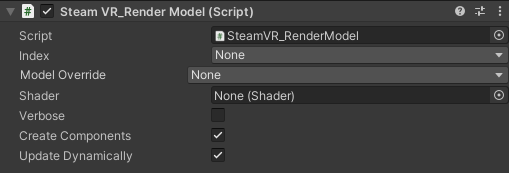
\includegraphics[scale=1]{pics/steamVR_render_models_script}
    \caption{Steam VR - Render Models Script}
    \label{fig:steamvr_render_models Script}
\end {figure}
Der Index ist der Index des getrackten Gerätes, und wird vom System wie eine ID zur Erkennung verwendet.
Mittels dem Model Override kann man für Testzwecke ein bestimmtes Modell festlegen, welches angezeigt werden soll.
Die Shader können die Darstellung des Objektes verändern.
Verbose gibt die Vorgänge im Script in der Konsole aus, diese Option wird jedoch nur für das Testen benötigt.
Create Components erstellt individuelle Objekte für jede Komponente, welche verfügbar ist.
Update Dynamically bewegt die einzelnen Komponenten gleich wie die physischen Gegenstücke.
~\cite{SteamVR_Render_Models_2022}

\subsection{Input}\label{subsec:input}
\setauthor{Florian Beckerle}
Die Hardware für VR Geräte schnell weiterentwickelt wird, hat Valve auf ein KeyBinding System zurückgegriffen.
Die Entwickler und die Benutzer selbst können für neue oder bereits vorhandene Hardware einstellen, welche Funktion die einzelnen Knöpfe und Trigger haben.
Diese Aktionen wurden in 6 verschiedene Input Typen und einen Output Typen aufgeteilt.

Die Aktion Boolean besitzt zwei Zustände, true und false.
Sie wird oft benutzt, um Objekte zu greifen, da man zum Beispiel einen Würfel entweder aufheben können soll oder nicht.

Single Aktionen können analoge Werte zwischen 0 und 1 annehmen und wird für Situationen benutzt, in denen der Boolean nicht ausreicht.
Ein Anwendungsfall ist ein Auto, welches bei 0 stehen bleibt und bei 1 Vollgas fährt.
Als Eingabe kann zum Beispiel der Trigger des Kontrollers benutzt werden.

Vector2 besitzt zwei Werte, X und Y.
Die Bewegungen des Kontrollers werden hierbei nur auf zwei Achsen gemessen.

Vector3 besitzt im Gegensatz zu Vector2 drei verschiedene Werte X, Y und Z.
Diese Aktion wird selten benutzt, findet aber zum Beispiel im SteamVR Home einen Anwendungsfall beim Scrollen.

Pose gibt die Position und Rotation in einem dreidimensionalen Raum wieder.
Es wird dazu benutzt, um die Bewegungen der Controller zu messen und digital nachzubilden.

Skeleton benutzt das SteamVR Skeleton Input, um die ungefähre Position und Rotation der Finger zu erkennen, während der Kontroller in den Händen gehalten wird.

Vibrationen werden für haptisches Feedback bei VR Geräten verwendet.
Hierbei vibrieren der Kontroller, eine spezielle Haptik Weste oder ein präparierter Sessel.
~\cite{SteamVR_Input_2022}

\subsection{Skeleton Input}\label{subsec:skeleton-input}
\setauthor{Florian Beckerle}
Das Plugin bietet die Möglichkeit, Hände mit Fingern und deren aktuelle Position darzustellen.
Die Bewegungen werden hierbei zwischen zwei verschiedenen Begrenzungen der Fingerpositionen unterschieden.
WithController berechnet eine ungefähre Position der Finger, während diese einen Kontroller in den Händen halten.
Dies dient besonders dazu, die Interaktion zwischen der realen Hand und dem realen Kontroller digital darzustellen.
WithoutController bietet die Bewegungen von Fingern, wenn sie keinen Kontroller in der Hand halten.
In der Realtität kann währenddessen jedoch trotzdem ein Kontroller gehalten werden, es wird nur digital nicht angezeigt, siehe Abb. ~\ref{fig:steamvr_skeletal_input_models}.
\begin {figure}
    \centering
    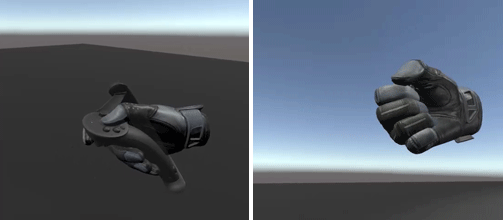
\includegraphics[scale=1]{pics/steamVR_skeletal_input_models}
    \caption{Steam VR - Skeletal Input Models}
    \label{fig:steamvr_skeletal_input_models}
\end {figure}
Die Positionen der Finger werden relativ zu dem in der Hierarchie übergestuften Objekt und dem Model gemessen.
Jeder Finger besteht hierbei standardmäßig aus 4 Gelenken.
Ein Wert im Bereich von 0 bis 1 gibt an, wie stark die Finger eingerollt sein sollen.
Die Finger einer Hand sind bei SteamVR etwas auseinandergestpreizt, hier wird ebenfalls ein Wert von 0 bis 1 dazu verwendet, um die Distanz zwischen den Fingern zu verändern.

Um die Position der Finger zu messen, gibt es grundsätzlich drei verschiedene Methoden.
Bei Estimated kann die Position des Körperteiles nicht direkt bestimmt werden.
Jede Bewegung wird nur über die Bediehnung der Trigger, Knöpfe und Trackpads des Kontrollers gestimmt.
Partial kann die Bewegungen der Finger direkt bestimmen, jedoch nur eingeschränkter als die tatsächlichen Finger.
Die Positionen werden durch andere Werte, wie zum Beispiel von speziellen Handschuhen, gemessen.
Full kann die komplette Körperbewegung des Benutzers messen, wie zum Beispiel durch Motion Caputre Anzüge oder Handschuhe.

Das Script, welches für die Bewegung des Modelles zuständig ist, besitzt eine Vielzahl an verschiedenen Optionen, siehe Abb. ~\ref{fig:steamvr_skeletal_input_Script}.
Update Pose setzt die Position und Orientierung des Objektes neu, sobald der Controller bewegt wurde.
Mirroring gibt an, ob die Knochen Daten entlang der X-Achse gespiegelt werden sollen.
Die Blend Optionen bieten Einstellungsmöglichkeiten, um den Übergang zwischen Verschiedenen Bewegungsmöglichkeiten und Animationen zu verändern.
Weiters kann man einen bestimmten Knochen mittels GetBonePosition bekommen und die Positionen und Rotationen werden mittels GetBonePositions und GetBoneRotations bereitgestellt.
\begin {figure}
    \centering
    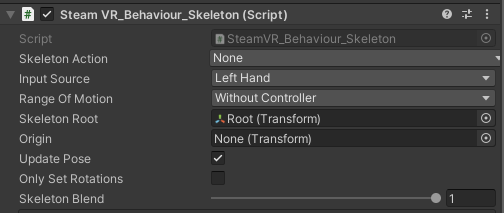
\includegraphics[scale=1]{pics/steamVR_skeletal_input_script}
    \caption{Steam VR - Skeletal Input Script}
    \label{fig:steamvr_skeletal_input_Script}
\end {figure}
~\cite{SteamVR_Skeleton_Input_2022}

\subsection{Interaction System}\label{subsec:interaction-system}
\setauthor{Florian Beckerle}
Das Interaction System funktioniert mittels dem Senden von Nachrichten an Objekte, mit welchen die Hände des Spielers oder andere Objekte interagieren.
Diese Objekte können sich an die Hand anheften und somit gehalten werden.
Das System bietet die Möglichkeit, Maus Events nachzuahmen, somit funktioniert die Interaktion mit der Benutzeroberfläche auch in VR.

Die Player Klasse weiß, wo die VR-Brille und die Kontroller positioniert sind.
Mittels der Methoden hmdTransform und feetPositionGuess können die Positionen der Brille und eine Schätzung der Fußstellung zurückgeliefert werden.

Die Hand Klasse wird für die meisten Funktionen des Interaction Systems benötigt.
Sie sendet interagierbaren Objekten Nachrichten über den aktuellen Status der Hand.
Sie kann nur mit einem Objekt gleichzeitig direkt interargieren, darunter versteht man das Aufheben und Werfen dieser.
Objekte können an die Hand angebracht und wieder losgelöst werden.
Das Verhalten der Hände kann durch sogenannte AttachmentFlags verändert werden, welche bei einer Interaktion aktiviert werden.

Interactable Objekte können von Spielern aufgehoben werden, solange ein bestimmter Knopf gedrückt wird.
Befindet sich die Hand, während dieser Knopf losgelassen wird, in Bewegung wird die Geschwindigkeit und die Richtung auf das Objekt übertragen und es wird geworfen.
%%Optional noch andere Scripts erklären falls notwendig, erscheinen jedoch nicht sonderlich wichtig (wichtigere noch mit !)
%    Throwable
%    LinearDrive
%    CircularDrive
%    LinearMapping
%    VelocityEstimator !!
%    IgnoreHovering
%    UIElement
%    ItemPackage
%    ItemPackageSpawner
%    ItemPackageReference
%    PlaySound
%    SoundPlayOneShot
%    Util
%    InteractableHoverEvents
%    InteractableButtonEvents
%    ComplexThrowable
%    DistanceHaptics
%    Player (Prefab) !!
%    BlankController (Prefab)
%    Teleport !!
%    Render Model
%    Hints
%    Samples
~\cite{SteamVR_Interaction_System_2022}

\subsection{Skeleton Poser}\label{subsec:skeleton-poser}
\setauthor{Florian Beckerle}
Der Skeleton Poser funktioniert mithilfe von verschiedenen Posen, welche erstellt und eingefügt werden können.
Mittels dem Blending Editor des Posers kann zwischen verschiedenen Posen ein Übergang erstellt werden.

Hierbei existieren 4 Modi für die Fingerbewegungen.
Der Static Modus erlaubt keine Fingerbewegungen und beachtet nur die Posen.
Bei Free können die Finger frei bewegt werden und die Pose wird ignoriert.
Mittels Extend können die Finger komplett ausgestreckt werden, aber nur nicht weiter eingerollt werden, als es bei der Pose eingestellt wurde.
Bei Contract können die Finger ganz eingerollt werden, jedoch nicht weiter ausgestreckt werden als bei der Pose.
~\cite{SteamVR_Skeleton_Poser_2022}

\subsection{OpenVR}\label{subsec:openvr}
OpenVR ist eine API, welche den direkten Zugriff auf VR-Hardware von verschiedenen Anbietern, wie Oculus, Mixed Reality und Vive, ermöglicht.
Hierbei benötigt die Anwendung keine speziellen Kenntnisse über die Hardware.
OpenVr besteht aus der Applikation und dem Treiber, welche über SteamVR miteinander kommunizieren.
Die API besteht aus mehreren C++ Interface Klassen.
Wenn die Applikation ausgeführt wird, liefert OpenVR, je nach vorhandenem SDK, das benötigte Interface zurück.
~\cite{OpenVR_Github_Documentation_2020}

\section{Final IK Plugin}\label{sec:final-ik-plugin}

Final IK ist ein Unity Asset, welches von RootMotion entwickelt wurde.
Es wurde kostenlos für die Erstellung von BeamVR bereitgestellt und regelt das Full Body Tracking.
Hierbei wird das Full Body Biped IK, welches inbegriffen ist, verwendet.
~\cite{FinalIK_Overview_2020}

\subsection{AimIK}\label{subsec:aimik}
AimIK rotiert die Knochen des 3D-Modells, sodass auf ein Objekt gezielt werden kann.
Es wird hierbei nicht die eingebaute LookAt Funktion des Animators benutzt, da die Objekte, mit denen gezielt wird, nicht mit den Achsen des Modells übereinstimmen.
AimIK ermöglicht ein natürlich aussehendes Ergebnis, selbst wenn sich das Ziel beinahe hinter dem zielendem Objekt befindet.
Rotation limits verhindern, dass das Skelett in unnatürliche Bewegungen und Stellungen verändert wird.
Bei menschenähnlichen Modellen limitiert diese Einstellung die Gelenke auf die gleichen Bewegungsmöglichkeiten wie bei einem Menschen, siehe Abb. ~\ref{fig:finalIK_aimIK_pose}.
Diese können jedoch frei verändert werden, was jedoch zu unrealistischen Posen führen kann.
\begin {figure}
    \centering
    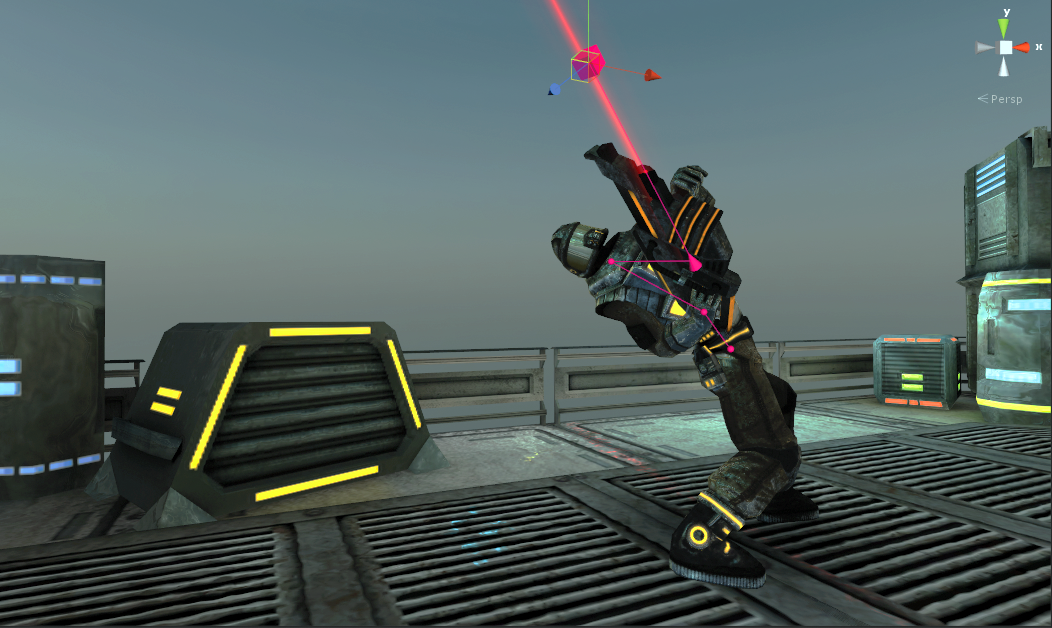
\includegraphics[scale=0.4]{pics/finalik_aimik_pose}
    \caption{Final IK - AimIK Pose}
    \label{fig:finalIK_aimIK_pose}
\end {figure}

Damit die Berechnung der Pose funktioniert, werden mehrere verschiedene Einstellungsmöglichkeiten bereitgestellt, siehe Abb. ~\ref{fig:finalIK_aimIK_script}.
Um zu wissen worauf gezielt werden soll, muss zuerst ein Ziel festgelegt werden, dies ist möglich bei der Variable Target.
Aim Transform ist das Objekt, mit welchem gezielt werden soll.
Dabei kann es sich um viele verschiedene Objekte, wie Waffen oder eine Hand, die auf etwas zeigen soll, handeln.
Axis gibt an, in welche Richtung das Objekt zielt.
Wenn zum Beispiel ein Laserpointer den Laser in Richtung der Z-Achse abstrahlt, muss die Achse auf (0,0,1) gesetzt werden, da das Schema (x,y,z) ist.
Damit die richtigen Knochen bewegt werden, wenn auf ein Ziel gezielt wird, müssen diese bei Bones definiert werden.
Das Wight steuert, wie stark die Veränderungen des Scripts auf die tatsächliche Position des Knochen einwirken sollen.
Bei 0 wird der Knochen kaum bis gar nicht verändert, wenn der Wert jedoch 1 ist, wird die ursprüngliche Position komplett verändert.
\begin {figure}
    \centering
    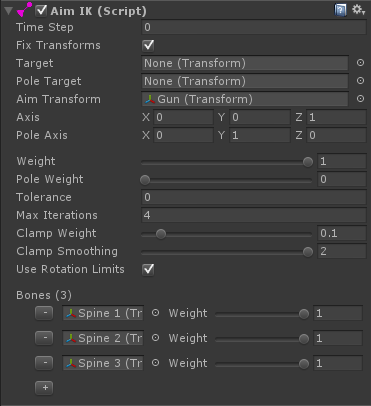
\includegraphics[scale=0.7]{pics/finalik_aimik_script}
    \caption{Final IK - AimIK Script}
    \label{fig:finalIK_aimIK_script}
\end {figure}
~\cite{FinalIK_AimIK_2021}

\subsection{Arm IK}\label{subsec:arm-ik}
ArmIK stellt die Position und Rotation der Knochen eines Armes so ein, dass die Hand möglichst nahe an der Zielposition platziert ist.
Hierfür werden 5 Knochen benötigt, Chest, Shoulder, Upper Arm, Forearm und Hand, siehe Abb. ~\ref{fig:finalIK_armIK_script}.
Chest befindet sich im Oberkörper des Modells und ist am nähesten am Arm dran.
Shoulder ist der Schulterknochen, Upper Arm ist der Oberarm Knochen, Forearm ist der Unterarm Knochen und Hand befindet sich in der Hand.
Hierbei werden die Finger nicht beachtet, da es sich nur um die Berechnung der Position des Armes handelt.
Mithilfe der Target Variable wird erneut ein Ziel festgelegt, welches die Zielposition der Hand angibt.
\begin {figure}
    \centering
    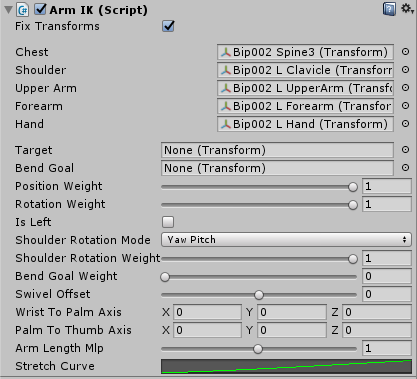
\includegraphics[scale=1]{pics/finalik_armik_script}
    \caption{Final IK - ArmIK Script}
    \label{fig:finalIK_armIK_script}
\end {figure}
~\cite{FinalIK_ArmIK_2021}

\subsection{Baker}\label{subsec:baker}
Der Baker ist ein Tool, welches die Aufnahme von Animations Clips ermöglicht.
Um humanoide Modelle aufzunehmen, muss das Humanoid Baker Script zu dem animierten Objekt hinzugefügt werden, siehe Abb. ~\ref{fig:finalIK_humanoid_baker}.
Für andere Modelle wird das Generic Baker Script benötigt, siehe Abb. ~\ref{fig:finalIK_generic_baker}.
Wenn die Applikation in Unity ausgeführt wird, kann in beiden Scripten auf Bake Animation States gedrückt werden.
Nun werden die Animationen in einen vorher ausgewählten Ordner abgespeichert und können jederzeit wiederverwendet werden.

\begin {figure}
    \centering
    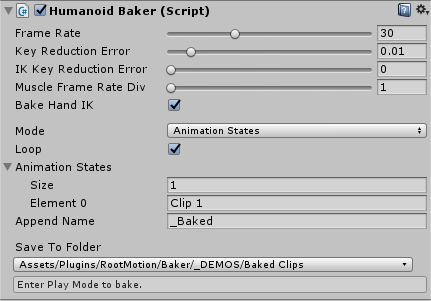
\includegraphics[scale=1]{pics/finalik_baker_HumanoidBakerComponent}
    \caption{Final IK - Humanoid Baker}
    \label{fig:finalIK_humanoid_baker}
\end {figure}
\begin {figure}
    \centering
    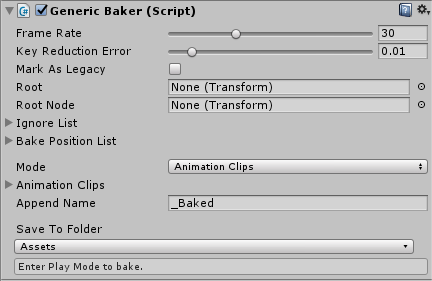
\includegraphics[scale=1]{pics/finalik_baker_GenericBakerComponent}
    \caption{Final IK - Generic Baker}
    \label{fig:finalIK_generic_baker}
\end {figure}
~\cite{FinalIK_Baker_2021}

\subsection{Biped IK}\label{subsec:biped-ik}
Biped IK erlaubt die Modifikation der Position und Rotation der Knochen eines Modelles mit 2 Beinen, 2 Armen und einem Kopf.
Das Script erkennt die Knochen automatisch und ist sofort einsatzbereit.
Seit FinalIK 4.0 wird jedoch FullBodyBiped IK empfohlen, da dieses eine leichtere Optimierung der IK eines Modelles erlaubt.

Es können wie bei vorherigen Funktionen Animationen beliebig überschrieben werden, ohne diese tatsächlich ändern zu müssen.
BipedIK bietet die Möglichkeit, jedes Glied, also Kopf, Füße, Arme, Ober- und Unterkörper, einzeln einzustellen, siehe Abb. ~\ref{fig:finalIK_bipedik_script}.
Weiters kann wieder ein Ziel festgelegt werden, falls der Charakter auf einen Gegenstand zielen soll.
\begin {figure}
    \centering
    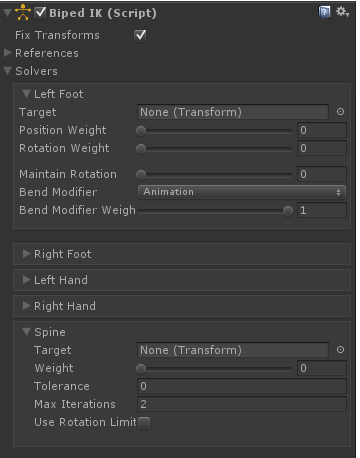
\includegraphics[scale=0.8]{pics/finalik_bipedik_script}
    \caption{Final IK - BipedIK Script}
    \label{fig:finalIK_bipedik_script}
\end {figure}
~\cite{FinalIK_BipedIK_2021}

\subsection{CCD IK}\label{subsec:ccd-ik}
Cyclic Coordinate Descent, auch als CCD bezeichnet, ist ein viel genutzter und bekannter Anwendungsfall von IK.
Dieses Script richtet die einzelnen Gelenke nacheinander in Richtung der Zielposition aus.
Durch das ständige Wiederholen dieser Aktion wird die Kette an Gelenken und Knochen richtig ausgerichtet.
Damit die Gelenke nicht unnatürliche Positionen einnehmen, kann ein Rotationslimit festgelegt werden, dieses kann nicht überschritten werden und sorgt für zusätzlichen Realismus.
Für längere Ketten an Gelenken wird empfohlen, FABRIK zu verwenden.
Ein Anwendungsfall für dieses Skript ist zum Beispiel ein Roboter oder andere Lebewesen, welche auf einem unebenen Gelände mit ihren Beinen auf dem Boden stehen sollen, siehe Abb. ~\ref{fig:finalIK_ccd_robot_example}.
Mit CCD ist es möglich die Beine so auszurichten, dass der Boden mit allen Gliedern berührt wird, ohne die Animationen anpassen zu müssen.
\begin {figure}
    \centering
    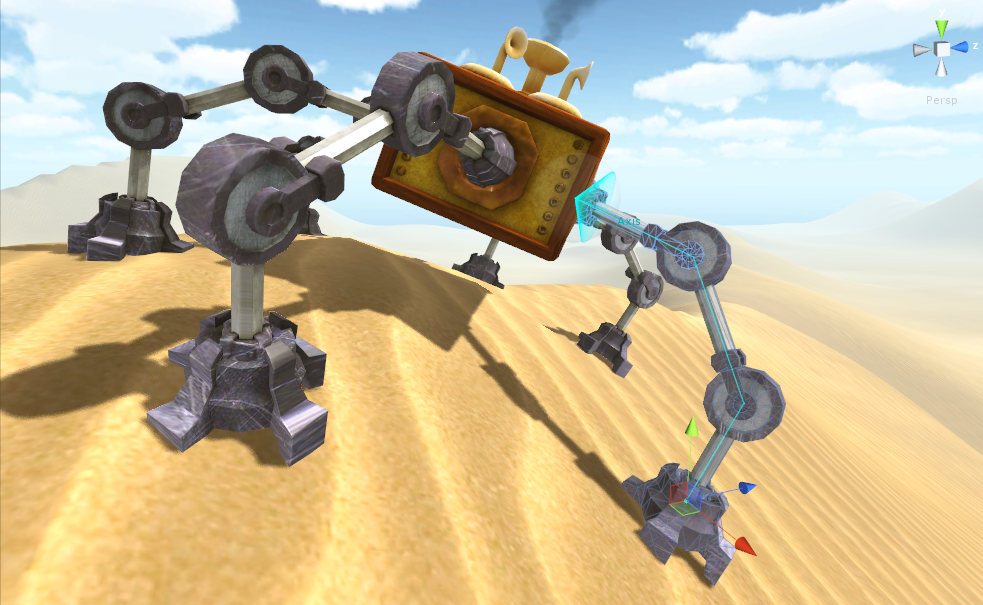
\includegraphics[scale=0.4]{pics/finalik_ccd}
    \caption{Final IK - CCD Robot Example}
    \label{fig:finalIK_ccd_robot_example}
\end {figure}
~\cite{FinalIK_CCD_2021}

\subsection{FABRIK}\label{subsec:fabrik}
Fabrik kann auf einer beliebigen Anzahl an Knochen-Segmenten mit Rotations-Limits verwendet werden.
Es benutzt eine Methode welche die neue Position von Gelenken in beide Richtungen, also Vorwärts und Rückwerts,
von einem Gelenk zum nächsten, berechnen kann.

Ein Vorteil von FABRIK ist, dass die Knochenlängen während der Laufzeit verändert werden können,
die Änderungen werden automatisch erkannt und neu berechnet. Ein Anwendungsfall für Fabrik ist in Abb. ~\ref{fig:finalIK_fabrik_example} zu sehen.
\begin {figure}
    \centering
    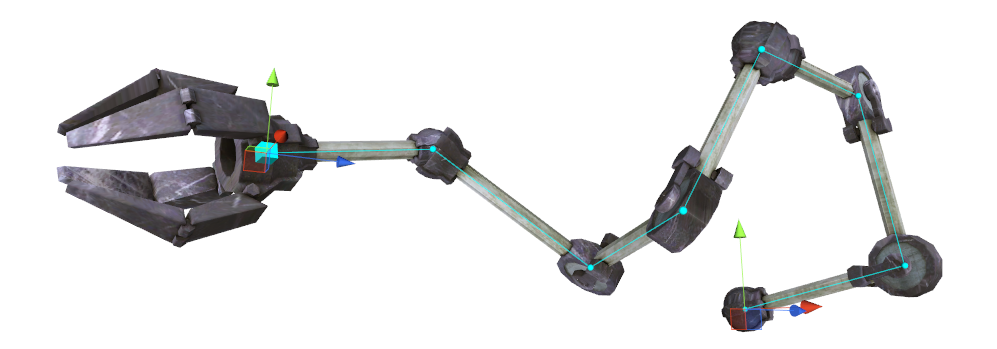
\includegraphics[scale=0.4]{pics/finalik_fabrik_pose}
    \caption{Final IK - Fabrik Example}
    \label{fig:finalIK_fabrik_example}
\end {figure}

Damit Fabrik benutzt werden kann, werden mehrere Variablen benötigt, siehe Abb. ~\ref{fig:finalIK_fabrik_script}.
Target, beschreibt die Position eines Zieles, zu welchem sich der Arm bewegen soll.
Die Position aller Knochen und Gelenke richtet sich automatisch so aus, dass der Arm auf das Ziel zeigt.

Weight kann dazu benutzt werden, um die Änderungen von Fabrik ein- und auszublenden. Ein Wert von 1 bedeutet,
dass alle Änderungen mit voller Kraft vorgenommen werden, wird der Wert nun näher an 0 gesetzt,
werden die Effekte nicht mehr übernommen.

Tolerance gibt die minimale Distanz an, welche die Zielposition bewegt werden muss,
bevor Fabrik die Berechnung aller Gelenke erneut startet. Liegt die Positionsänderung unter dem
Toleranzbereich wird nichts unternommen.

MaxIterations gibt die maximale Anzahl an Iterationen, welche in einem Frame durchgeführt werden dürfen.
Während den Iterationen wird die Position der Knochen und Gelenke berechnet.

UseRotationLimits gibt an, ob die Rotationslimits auf den Einzelnen Knochen bei der Berechnung der Position
miteinbezogen werden sollen, oder nicht.

Bei Bones, handelt es sich um eine Liste, welche alle Knochen beinhalten soll, die bei der Berechnung der
Positionen und Rotationen, herangezogen werden sollen.
~\cite{FinalIK_FABRIK_2021}
\begin {figure}
    \centering
    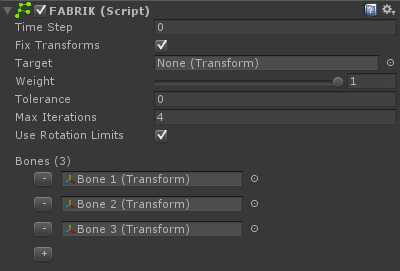
\includegraphics[scale=0.8]{pics/finalik_fabrik_script}
    \caption{Final IK - Fabrik Script}
    \label{fig:finalIK_fabrik_script}
\end {figure}


\subsection{FABRIK Root}\label{subsec:fabrik-root}


Fabrik Root ist ein Component, welcher mehrere einzelne Fabrik Ketten miteinander verbinden lässt.
Hierbei kann es sich um kompliziertere Systeme mit mehreren Abzweigungen handeln, siehe Abb. ~\ref{fig:finalIK_fabrik_root_example}

\begin {figure}
    \centering
    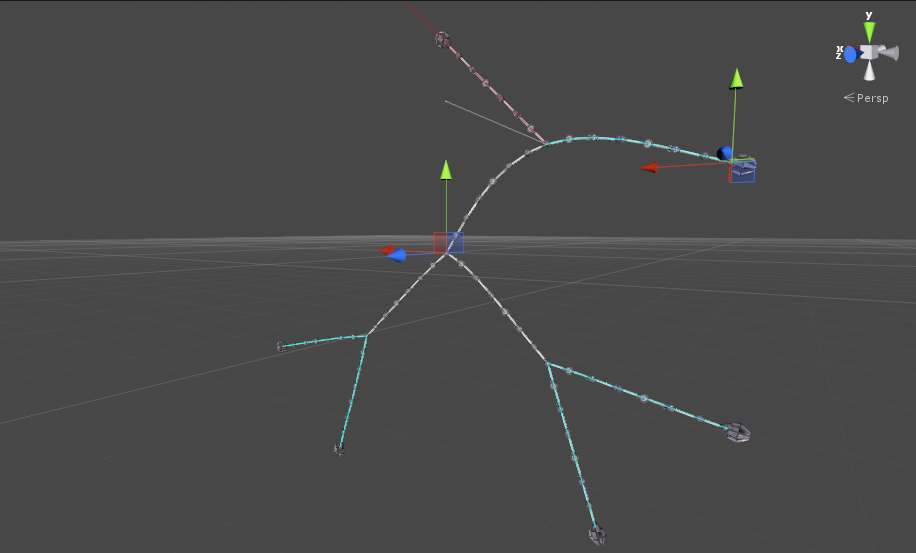
\includegraphics[scale=0.8]{pics/finalik_fabrik_root_example}
    \caption{Final IK - Fabrik Root Script}
    \label{fig:finalIK_fabrik_root_example}
\end {figure}


Damit Fabrik Root richtig funktioniert müssen, ähnlich wie bei Fabrik, verschiedene Variablen angegeben werden,
siehe Abb. ~\ref{fig:finalIK_fabrik_root_script}.

Weight wird benutzt, um die Änderungen von FabrikRoot und Fabrik ein- und auszublenden.
Ein Wert von 1 bedeutet, dass alle Änderungen mit voller Kraft vorgenommen werden, wird der Wert nun auf 0 gesetzt,
werden die Effekte nicht mehr übernommen.

Iterations gibt die Anzahl an Iterationen, welche in einem Frame durchgeführt werden dürfen, an.
Hierbei wird in jeder Iteration die Position und Rotation aller angegebenen Fabrik Ketten berechnet.

RootPin befestigt die Fabrik Ketten an einen Bestimmten Ort, welcher zum Beispiel auf einem Objekt,
oder irgendwo in der Luft platziert werden kann. Dieser Punkt kann nicht durch die Fabrik Ketten bewegt werden.

Chains ist eine Liste an Fabrik.
IK gibt den Fabrik Komponent an, welcher die Position und Rotation einer Knochenkette berechnet.

Pull gibt an wie stark diese Kette die, in der Hierarchie übergestellte, Kette bewegen darf.

Pin gibt an, wie stark die Kette von einer Kette, welche in der Hierarchie untergeordnet ist, bewegt werden kann.

Children ist eine Liste von Indizes, welche auf die, in der Hierarchie untergeordneten, Fabrik verweist.

\begin {figure}
    \centering
    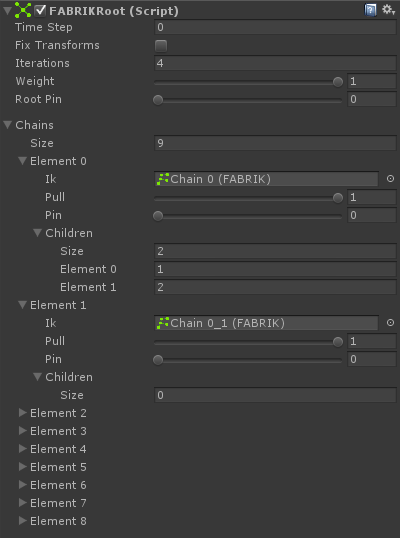
\includegraphics[scale=0.5]{pics/finalik_fabrik_root_script}
    \caption{Final IK - Fabrik Root Script}
    \label{fig:finalIK_fabrik_root_script}
\end {figure}

\subsection{Full Body Biped IK}\label{subsec:full-body-biped-ik}
Die Full Body Biped IK ist eine flexible und schnelle Lösung für Biped Charaktere, darunter Fallen Modelle, welche zum Beispiel auf zwei Beinen stehen.
Der Charakter wird auf ein simples IK-Rig reduziert, von welchem die Position und Rotation der einzelnen Gliedmaßen berechnet wird.
Die Berechnung wird dabei in jedem Frame durchgeführt.
Das Ergebnis danach wieder auf das 3D Modell übertragen, siehe Abb. ~\ref{fig:finalIK_full_body_biped_ik}.
~\cite{FinalIK_FullBodyBipedIK_2021}

\begin {figure}
    \centering
    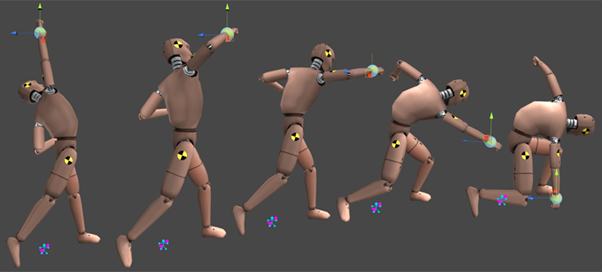
\includegraphics[scale=0.5]{pics/fullbodybipedIK}
    \caption{Final IK - FullBodyBiped IK}
    \label{fig:finalIK_full_body_biped_ik}
\end {figure}


\begin{spacing}{1}
	\chapter{Code Implementierung}
	\label{ch:code-implementation}
\end{spacing}
\section{Full-Body-Tracking}
\label{sec:full-body-tracking}
\setauthor{Quirin Ecker}

Das Full-Body-Tracking wurde mit einem kostenpflichtigen Plugin namens Final IK implementiert.
Dieses Plugin ist für die Arbeit gratis zur Verfügung gestellt worden.

Bevor Full-Body-Tracking benutzt werden kann, muss das Tracking erstmals kalibriert werden.
In BeamVR funktioniert die Kalibration des Full-Body-Trackings mit dem Trackpad auf dem Controller.
Diese Taste ist in Abb.~\ref{fig:vive-controller-trackpad} zu sehen.
Die Taste für das Kalibrieren wird in der Inbetriebnahme, welche in Abschnitt~\ref{ch:commisioning} beschrieben wird, benutzt.

Standardmäßig wird in FinalIK das Full Body Tracking mit der Taste C kalibriert.
Damit die Kalibration auch in VR erfolgen kann, ist eine Taste für das kalibrieren auch auf dem Controller reserviert.
Wie bereits beschrieben ist diese Taste das Trackpad auf dem Controller.

Um das Kalibrieren auf eine andere Taste zu stellen, werden die Daten für das Full-Body-Tracking an die eine Script-Komponente übergeben.
Diese Script-Komponente horcht auf Tastenbetätigungen des Trackpad.
Sobald die Taste gedrückt wird, wird die statische Funktion \emph{Calibrate()} der Klasse \emph{Calibrate()} mit den übergebenen Daten aufgerufen.

Um zu checken, ob die Taste gedrückt wird, benützen wir das SteamVR Plugin.
In Listing~\ref{lst:defining-control-objects} werden die Objekte für das Kontrollieren der Tasten zugewiesen.
Mit diesen Objekten kann mithilfe der Update-Methode auf einen Tastendruck gehorcht werden.
Das Horchen auf diese Taste ist in Listing~\ref{lst:checking-for-input} ersichtlich.
In diesem Fall muss auf die Taste beider Controller gehorcht werden, weshalb hier auf zwei Tasten gehorcht wird.

\begin{lstlisting}[language={[Sharp]C},label={lst:defining-control-objects}, caption={Zuweisung der Kontroll Objekt}]{Zuweisung der Kontroll Objekte}
private readonly SteamVR_Action_Boolean _inputAction = SteamVR_Actions.default_Teleport;
private const SteamVR_Input_Sources RightController = SteamVR_Input_Sources.RightHand;
private const SteamVR_Input_Sources LeftController = SteamVR_Input_Sources.LeftHand;
\end{lstlisting}

\begin{lstlisting}[language={[Sharp]C},label={lst:checking-for-input}, caption={Auf Nutzerinput warten}]{Auf Nutzerinput warten}
private void Update()
{
    if (_inputAction.GetStateDown(RightController) || _inputAction.GetStateDown(LeftController))
    {
        // Calibrate();
        ...
    }
}
\end{lstlisting}

Wie bereits beschrieben werden die Daten der Script-Komponente übergeben.
Das Object welches diese Daten hält ist von dem Typen \emph{VRIKCalibrationController}.
Dieses wird schlussendlich wie in Listing~\ref{lst:vrik-calibration} verwendet.

\begin{lstlisting}[language={[Sharp]C},label={lst:vrik-calibration}, caption={Kalibrierung}]{Kalibrierung}
_calibrationControllerObject.data = VRIKCalibrator.Calibrate(
    _calibrationControllerObject.ik,
    _calibrationControllerObject.settings,
    _calibrationControllerObject.headTracker,
    _calibrationControllerObject.bodyTracker,
    _calibrationControllerObject.leftHandTracker,
    _calibrationControllerObject.rightHandTracker,
    _calibrationControllerObject.leftFootTracker,
    _calibrationControllerObject.rightFootTracker
);
\end{lstlisting}

\section{Schwerkraft}
\label{sec:gravity}

Damit die Applikation eine gewisse Spannung erhält, gibt es auch die Möglichkeit von dem Balken runterzufallen.
Dies sollte passieren, sobald die Person auch in der physischen Realität von dem Balken fällt.
Folgend ist die Bedingung für einen Fall beschrieben.

\subsection{Bedienung}\label{subsec:bedienung}

Bei der implementierung des Fallens muss es bestimmte Bedienungen geben, bei denen die Spielerin oder der Spieler herunterfallen soll.
Die erste Bedienung ist, dass die Benutzerin oder der Benutzer sich über dem Abgrund befindet.
Befindet sich die Person noch auf dem Haus, steht sie zwar nicht auf dem Balken, sollte aber trotzdem nicht herunterfallen.

Die zweite Bedingung ist, ab wann eine Person, welche sich über dem Abgrund befindet, von dem Balken herunterfliegt.
Grundsätzlich fliegt die Benutzerin oder der Benutzer von dem Balken, wenn diese oder dieser das Gleichgewicht verliert.
Der einfachheitshalber wurde keine Bedingung anhand des Gleichgewichtes implementiert.

Schlussendlich musste die Entscheidung getroffen werden, ob die Benutzerin oder der Benutzer bereits bei einem Fuß der bei zwei Füßen am Boden herunterfliegt.
In der BeamVR Applikation ist die Entscheidung auf die Bedingung mit einem Fuß auf dem Boden gefallen.
Somit fällt die Benutzerin oder der Benutzer von dem Balken herunter, sobald ein Fuß der Person auf dem Boden ankommt.

\subsection{Funktionsweise}\label{subsec:funktionsweise}

\begin{figure}
    \centering
    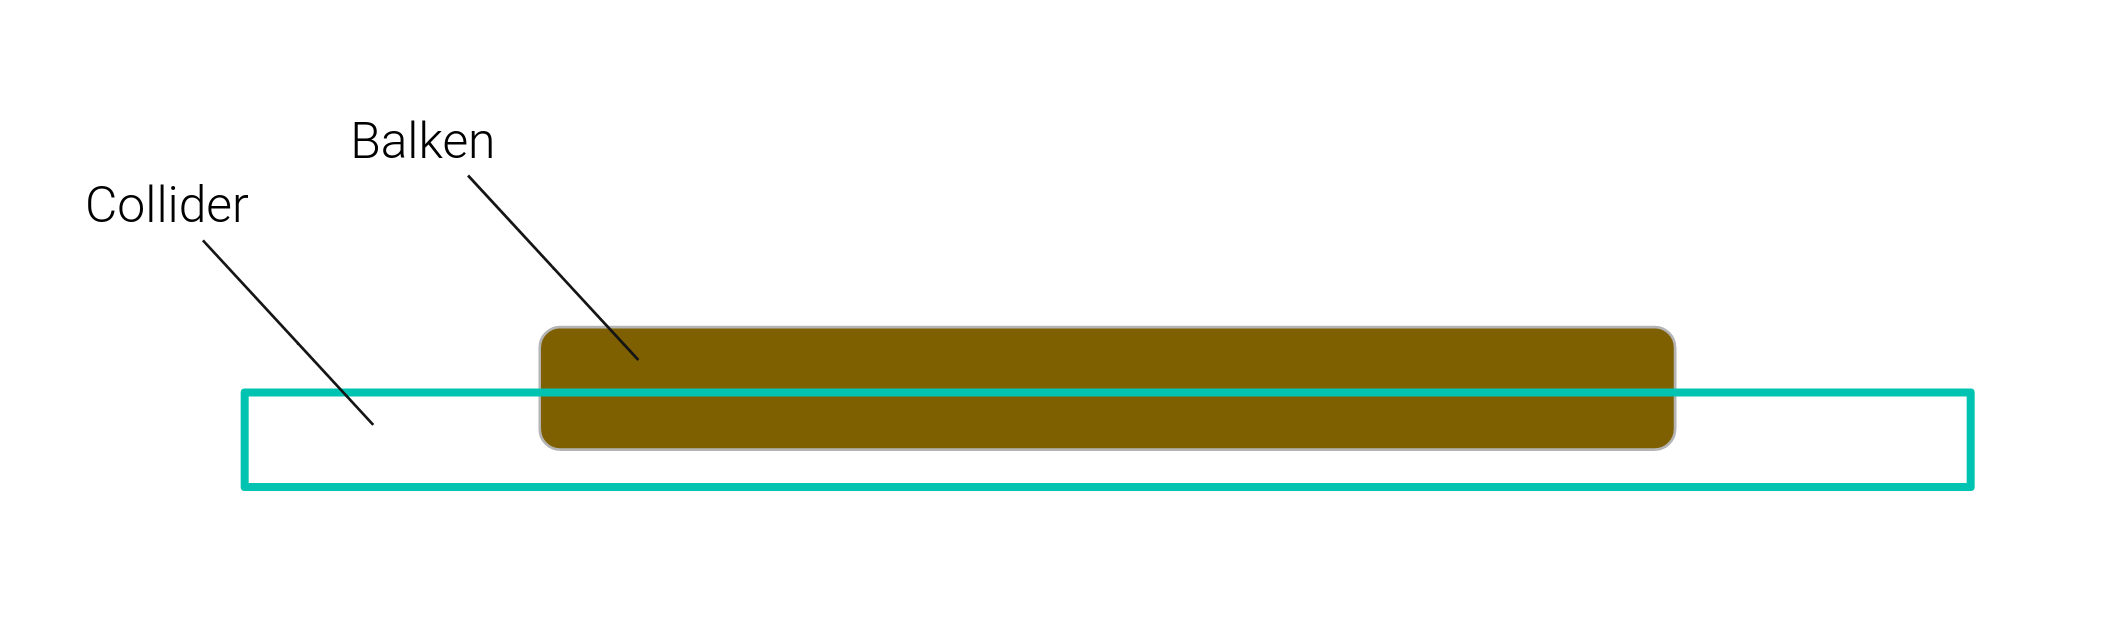
\includegraphics[scale=0.2]{pics/gravitation_collider}
    \caption{Schwerkraft Collider}
    \label{fig:gravitation-collider}
\end{figure}


Um zu checken, ob ein Fuß sich auf dem Boden befindet wurde ein Collider unter den Balken in der Höhe des Bodens platziert.
Diesen Collider ist eine unsichtbare Box, die nur für die Überprüfung möglicher Kollision existiert.
In Abb.~\ref{fig:gravitation-collider} ist diese Anordnung visualisiert.

Die Höhe des Bodens wird durch das SteamVR Setup ermittelt.
Hier werden die Kontroller auf den Boden gelegt und in dem Setup auf Kalibrieren gedrückt, um die Höhe des Bodens zu ermitteln.
Dies funktioniert anhand der getrackten Controller.
Weitere Informationen über das SteamVR Setup können in Abschnitt~\ref{sec:steam-vr-setup} gefunden werden.

Kollidiert einer der Füße mit dem Collider, wird die gesamte VR Fläche mit einer Beschleunigung von 9.81 m/s nach unten bewegt.
Kurz bevor die Fläche auf dem Boden aufkommt, wird in eine ander Szene gewechselt.

Um die Möglichkeit zu verhindern, dass der Kopf durch das Haus fliegt, da nur die füße sich auf dem Boden befinden und der Kopf immer noch über dem Haus wurde ein weiterer Check eingebaut.
Dieser Check beinhaltet, dass das Headset sich über dem Collider befinden muss, damit die Spielerin oder der Spieler runterfliegt.
Befindet sich das Headset noch über dem Haus kann der Spieler oder die Spielerin nicht von dem Haus fliegen.

\section{Verkehrssystem}
\label{sec:traffic-system}
\setauthor{Florian Beckerle}
In der Stadt von BeamVR ist auf den Straßen einiges los, dass wurde mithilfe eines neuen Verkehrssystems umgesetzt.
Die Straßen sind mit, f\"ur den Spieler unsichtbaren, Objekten versehen, die den Verkehr regeln.

\textbf{Car Signals}
Damit die Fahrzeuge in BeamVR wissen wo und vor allem wie sie auf den Straßen navigieren k\"onnen, wurde das Car Signal System entwickelt.
Die Car Signals gibt es in zwei verschiedenen Versionen, f\"ur die linke Straßenseite wurden gr\"une und f\"ur die rechte Seite wurden rote Signale erstellt.
Die Signale funktionieren wie Checkpoints.
Jedes Auto wird, nachdem es initialisiert wurde, von einem zum n\"achsten fahren.
Jeder dieser Checkpoints verweist auf den nächsten, wie in einer Liste, daher weiß jedes Fahrzeug, wo die momentane Zielposition ist.~\ref{fig:trafficsystem_next_signal_reference}
Endpunkte sind spezielle Signale, welche auf keinen nachfolgenden Punkt mehr verweisen.
Erreicht ein Auto ein solchen Punkt, hat es das Ziel erreicht.

An Kreuzungen befinden sich mehrere dieser Car Signals, damit die Fahrzeuge auf der richtigen Spur bleiben und die Verkehrsregeln befolgen.
Die gr\"unen Linien zeigen die m\"oglichen Routen, die das Auto fahren kann.
Die Pfeile visualisieren, in welche Richtung gefahren werden kann, siehe Abb.~\ref{fig:trafficsystem_crossroads}.


\begin{figure}
    \centering
    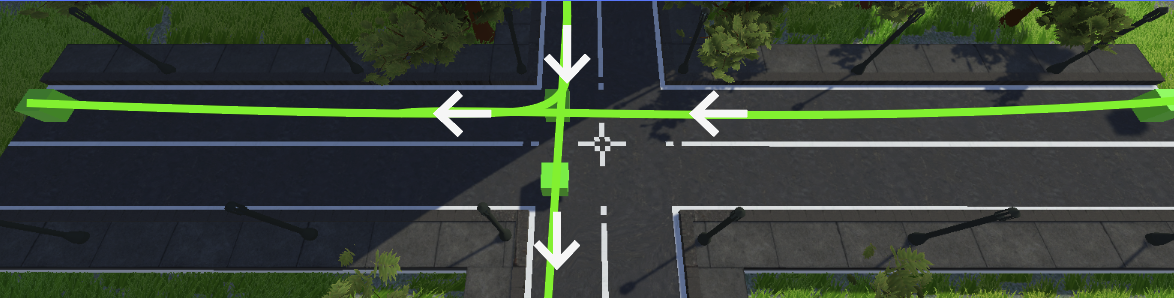
\includegraphics[scale=0.5]{pics/trafficsystem_carsignal_crossroads}
    \caption{Traffic System - Crossroads}
    \label{fig:trafficsystem_crossroads}
\end{figure}

\begin{figure}
    \centering
    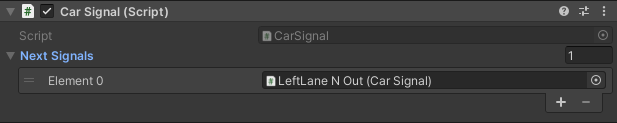
\includegraphics[scale=0.7]{pics/trafficsystem_carsignal_signal_reference}
    \caption{Traffic System - Next Signal Reference}
    \label{fig:trafficsystem_next_signal_reference}
\end{figure}


\textbf{Car Spawn Points}
Car Spawn Points sind blau dargestellte Punkte, an denen Fahrzeuge nach dem Laden der Szene initialisiert werden, siehe Abb.~\ref{fig:trafficsystem_car_spawn_points}.
Falls ein Auto einen Car Signal, welcher ein Endpunkt ist, erreicht, wird es nach einem kurzen Delay an einem Respawn Point wieder erscheinen.
Diese Punkte verweisen, \"ahnlich wie Car Signals, auf einen nachfolgenden Punkt, wo die Fahrzeuge hinfahren.

%% IN QUELLCODEVERZEICHNIS PACKEN!
\begin{lstlisting}{CarSpawnPoint.cs}
public class CarSpawnPoint : MonoBehaviour
{

    //Location where the car should go after respawning
    public CarSignal nextSignal;

    //Position of the Respawnpoint;
    public Vector3 position;

    public void Start(){
        position = transform.position;
    }

    public Vector3 GetPosition(){
        return position;
    }

    public CarSignal GetNextSignal(){
        return nextSignal;
    }

}
\end{lstlisting}

\begin{figure}
    \centering
    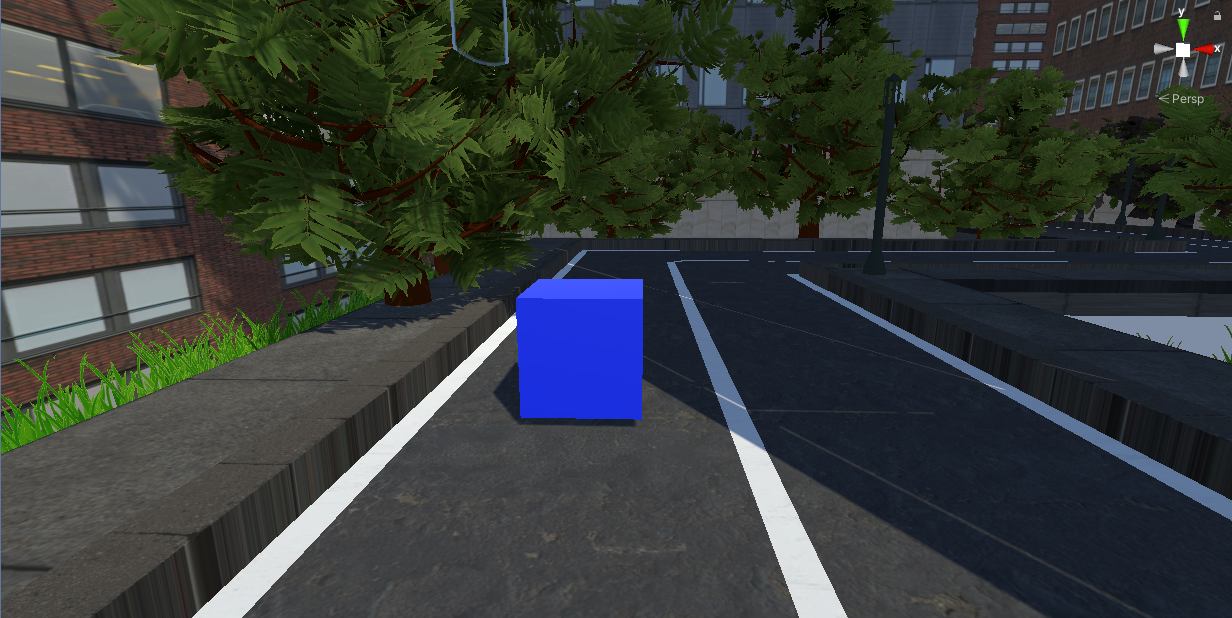
\includegraphics[scale=0.4]{pics/trafficsystem_respawn_point}
    \caption{Traffic System - Car Spawn Points}
    \label{fig:trafficsystem_car_spawn_points}
\end{figure}


\textbf{Car Manager}
Der Car Manager regelt die maximale Anzahl an Fahrzeugen die gleichzeitig auf den Straßen fahren k\"onnen.
Am Anfang werden n Fahrzeuge (n ist hierbei die maximale Anzahl an Autos) auf den Straßen initialisiert, indem ein zuf\"alliger Spawn Point ausgewählt wird.
\begin{lstlisting}{car_manager_respawncars}

public void SpawnCar(){
        CarSpawnPoint newCarSpawnPoint = GetRandomSpawnPoint();
        GameObject newCar = Instantiate(GetRandomCarModell(), newCarSpawnPoint.GetPosition(), newCarSpawnPoint.transform.rotation);
        newCar.GetComponent<CarBehaviour>().SetCarManager(this);
        CarBehaviour carBehaviour = newCar.GetComponent<CarBehaviour>();


        carBehaviour.curSignal = newCarSpawnPoint.GetNextSignal();
        carBehaviour.curPosition = newCarSpawnPoint.GetPosition();

        currentCars.Add(newCar);
    }
\end{lstlisting}

Weiters wird mithilfe der Funktion RespawnCars() ein Auto recycled, sobald es einen Endpunkt erreicht hat, indem der Manager die aktuelle Position und das n\"achste Ziel des Fahrzeuges neu setzt.
\begin{lstlisting}{car_manager_respawncars}
public void RespawnCars(GameObject finishedCar){
        CarBehaviour carBehaviour = finishedCar.GetComponent<CarBehaviour>();
        CarSpawnPoint newCarSpawnPoint = GetRandomSpawnPoint();
        carBehaviour.curSignal = newCarSpawnPoint.GetNextSignal();
        carBehaviour.curPosition = newCarSpawnPoint.GetPosition();
    }
\end{lstlisting}

\textbf{Car Behaviour}
Jedes Fahrzeug erh\"alt, nachdem es initialisiert wurde, eine zufällige ID mit folgendem Aufbau "Car[0-9]BeamVR[0-9]", damit diese im sp\"ateren Verlauf des Spieles besser identifiziert werden können.
In jedem Frame bewegt sich das Auto mithilfe der Vector3.MoveTowards() Funktion in Richtung dem Car Signal, welches als Ziel festgelegt wurde.
Wenn nun das momentane Ziel erreicht wurde, sucht das Gefährt in dem aktuellen Punkt die Referenz auf das nächste Signal und bewegt sich dorthin.

Um zu verhindern, dass mehrere Fahrzeuge ineinander fahren, kann das Auto mithilfe eines Raycasts erkennen, was sich in einer bestimmten Distance vor ihm befindet und im Notfall anhalten.

\begin{lstlisting}{car_behaviour_raycast}
...
RaycastHit hit;
         if (!Physics.Raycast(curPosition, transform.TransformDirection(Vector3.forward), out hit, carSeeingDist, layerMask))
        {
        ...
        }
...
\end{lstlisting}

\section{Beam Kalibration}
\label{sec:beam-calibration}
\setauthor{Quirin Ecker}

Das Kernthema dieser Arbeit ist, ein reales Objekt in die virtuelle Welt zu synchronisieren.
Im Falle unserer Arbeit ist dieses Objekt wie bereits beschrieben ein Balken.

Die Beam Kalibration ist für die Synchronisation des physischen und virtuellen Balkens zuständig.
In der Entwicklungsphase gab es mehrere Ansätze diese Synchronisation zu implementieren.
Hier ist zwischen Grundansätzen und Implementierungsansätze zu unterscheiden.
Im Zuge dieser Arbeit beschreibt ein Grundansatz die grundlegende Strategie das Problem zu lösen und ein Implementierungsansatz die Strategie einen Grundansatz zu lösen.

\subsection{Grundansätze}\label{subsec:grundansaetze}

Folgend werden zwei dieser Grundansätze beschrieben.

\subsubsection{Tracker Ansatz}

Der Initial-Ansatz dieser Arbeit war der \emph{Tracker Ansatz}.
Dieser Ansatz war eine Lösung mit den Vive Trackern.
In diesem Lösungsansatz würde ein Tracker in die Mitte des Balkens platziert werden.
Durch diesen Tracker und die Dimensionen des Balkens würde es in der Theorie möglich sein die Position und größe des Balkens zu berechnen.

Der Vorteil dieses Ansatzes wäre, dass der Balken während des Spielerlebnis verschiebbar ist, da die Position durch den Tracker aktualisiert werden kann.

Leider besitzt dieser Ansatz durch die Benutzung des Trackers einige Nachteile.
Einer dieser Nachteile ist, dass die Dimensionen des Balkens beim Initial Setup gemessen werden müssen.
Weiters muss der Tracker in der mitte des Balkens befestigt werden, da durch Änderungen der Position des Trackers auch Änderungen des virtuellen Balkens auftreten.
Bei keiner Befestigung kann der Tracker leicht verrutschen.
Schlussendlich muss auch die Mitte des Balkens ermittelt werde, um den Tracker dort zu platzieren.
Wenn die Ermittlung ungenau ist, wird es zu einer ungenauen Synchronisation führen.

\subsubsection{Marker Ansatz}

Für die BeamVR Applikation reicht es normal aus, dass die Skalierung, Position und Orientierung einmal vor dem Spielerlebnis ermittelt werden.
Das bedeutet, dass die dynamische Änderung der Position in den meisten Fällen vernachlässigt werden kann.

Bei dem Marker Ansatz werden keine zusätzlichen Geräte wie Tracker gebraucht.
Für das Kalibrieren des Balkens wird dabei einer der Controller verwendet

Im Prinzip wird bei diesem Ansatz der Controller verwendet, um die Ecken des Balkens zu markieren.
Diese Markierungen werden von der Applikation gespeichert und später in der Game-Szene verwendet, um den Balken richtig zu positionieren, skalieren und orientieren.
Da die Höhe durch das SteamVR Setup bekannt ist, müssen nur die oberen Ecken des Balkens.
Für mehr Informationen über das SteamVR Setup wird auf den Abschnitt~\ref{sec:steam-vr-setup}.

\begin{figure}
    \centering
    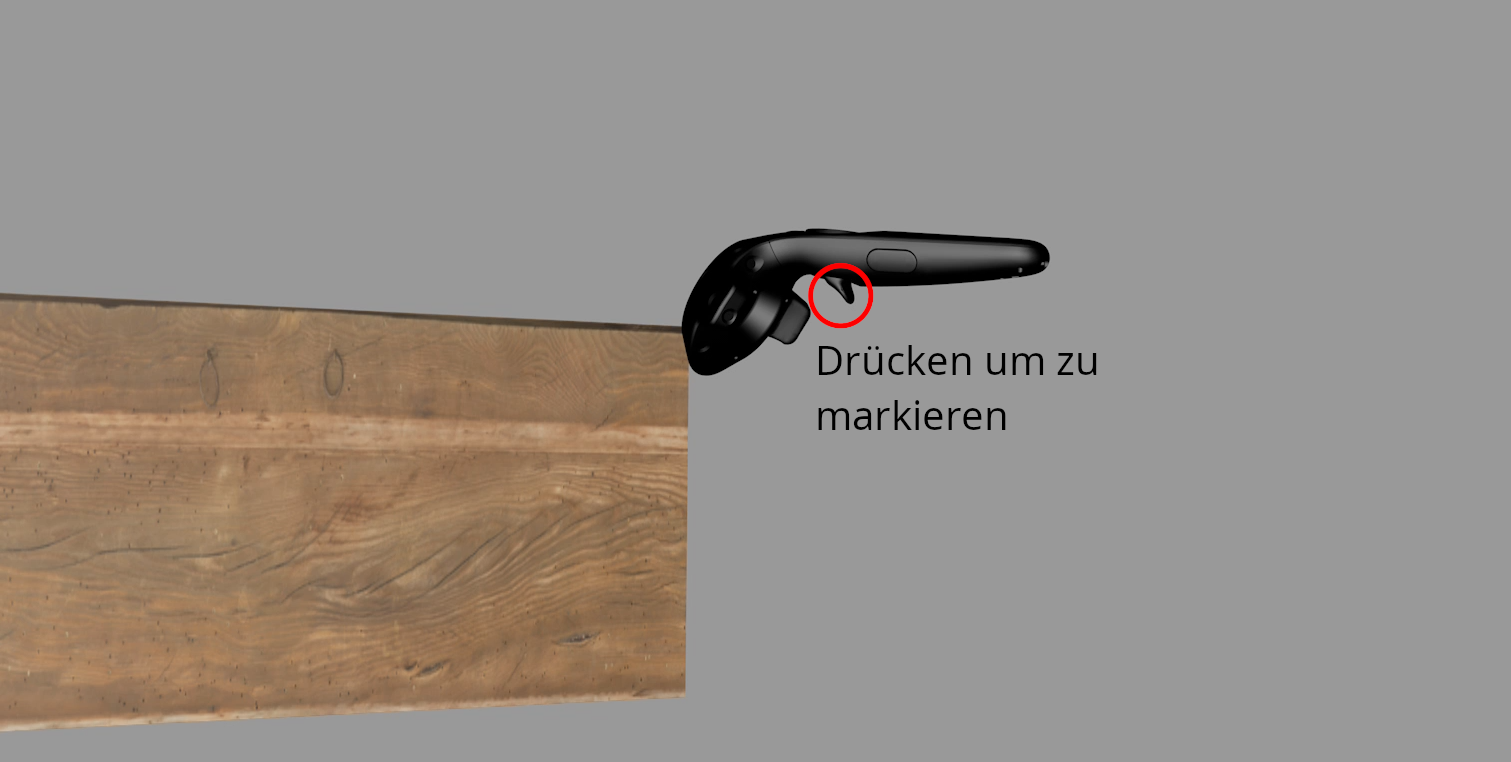
\includegraphics[scale=0.3]{pics/beam_mark}
    \caption{Markierung Einer Ecke des Balkens}
    \label{fig:beam-mark}
\end{figure}

Eine dieser Markierung wird folgendermaßen durchgeführt.
Der Ring am Ende des Controller muss an der gewünschten Ecke anstoßen.
Daraufhin wird der Trigger gedrückt, welcher sich an der unteren seite des Controller befindet.
In Abb.~\ref{fig:beam-mark} ist dieser Vorgang dargestellt.

\begin{figure}
    \centering
    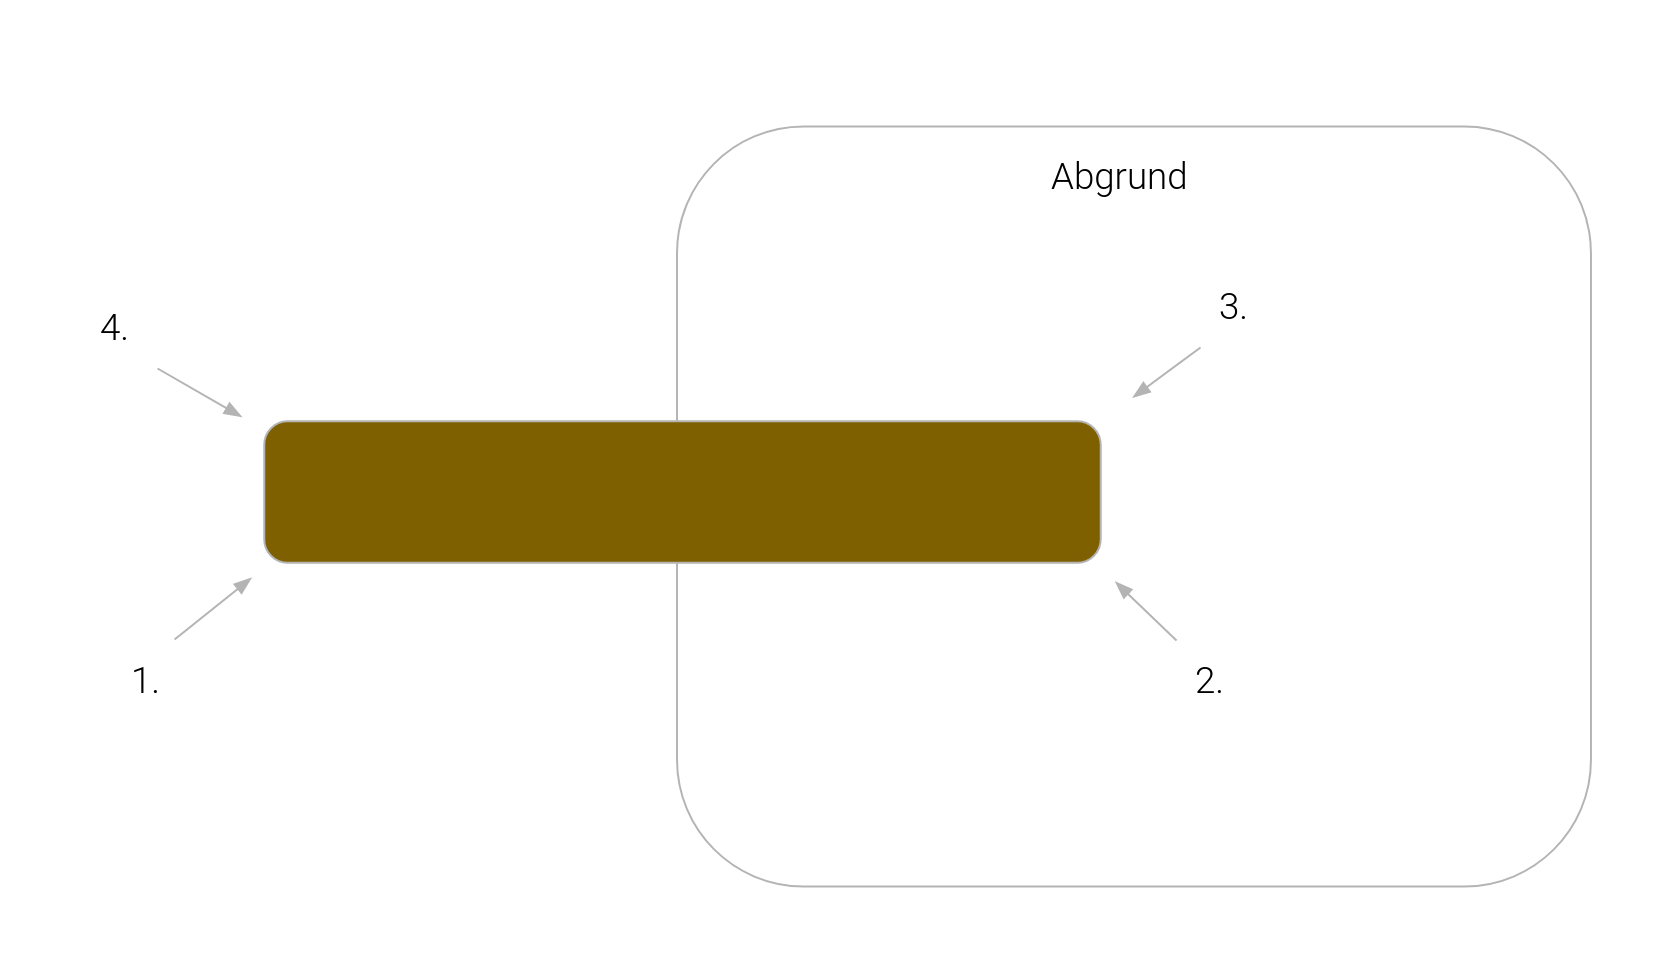
\includegraphics[scale=0.25]{pics/beam-marking-sequence}
    \caption{Reihenfolge der Markierungen}
    \label{fig:beam-marking-sequence}
\end{figure}

Insgesamt muss jede obere Ecke mit dem zuvor beschriebenen Vorgang markiert werden.
Für die Markierung jeder Ecke gibt es eine gewisse Reihenfolge.
Diese Reihenfolge ist von der BeamVR Applikation vordefiniert und von der Position des Abgrunds abhängig.
In Abb.~\ref{fig:beam-marking-sequence} ist die Reihenfolge ersichtlich.

Da die dynamische Positionsänderung während der Laufzeit in der BeamVR Applikation vernachlässigt werden kann wurde der Marker-Ansatz für die finale Applikation gewählt.

\subsection{Basisberechnungen}
\label{subsec:basisberechnungen}

\begin{figure}
    \centering
    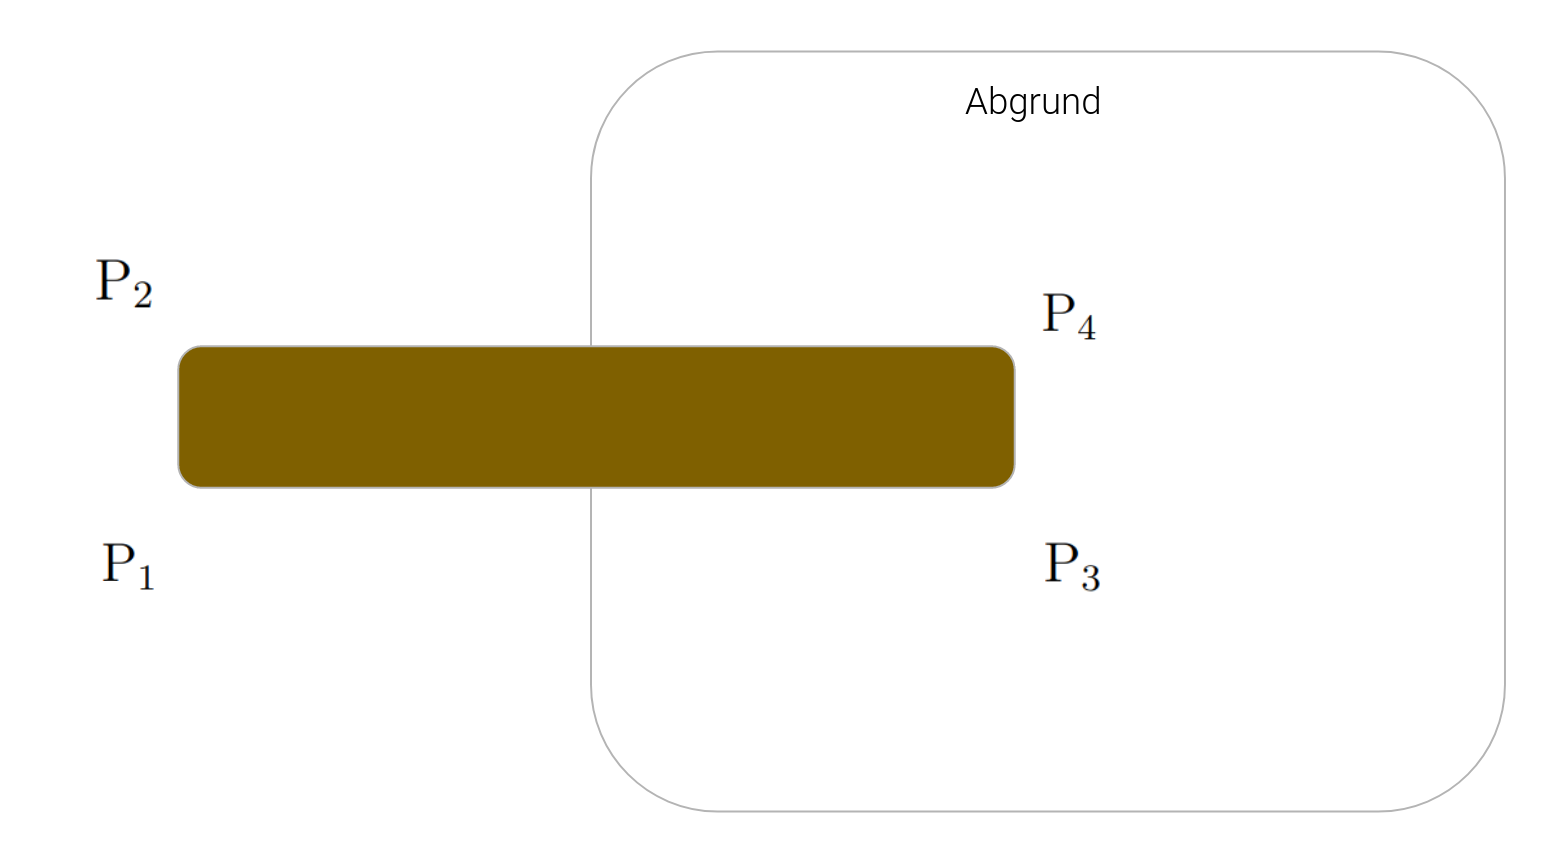
\includegraphics[scale=0.25]{pics/beam-point-labeling}
    \caption{Beschriftungen des Balkens}
    \label{fig:beam-point-labeling}
\end{figure}


Durch die Postionen der Ecken kann die Mitte des Balkens berechnet werden, da davon ausgegangen werden kann, dass der Balken ein Quader ist.
In Abb.~\ref{fig:beam-point-labeling} sind die Ecken der oberen Seite des Balken mit $P_{1}, P_{2}, P_{3}, P_{4}$ beschriftet.
Diese Punkte beschreiben die Reihenfolge, in der die Punkte der unteren seite $O_{1}, O_{2}, O_{3}, O_{4}$ und der oberen Seite $U_{1}, U_{2}, U_{3}, U_{4}$ angeordnet sind.
Alle restlichen Variablen können in der Tabelle~\ref{tab:variables} eingesehen werden.
Die Mitte der oberen Decke kann mit der folgenden Formeln berechnet werden.

\begin{table}[]
    \centering
    \begin{tabular}{|l|l|}
        \hline
        $O_{1}, O_{2}, O_{3}, O_{4}$ & Ecken der oberen Seite des Balkens                 \\ \hline
        $U_{1}, U_{2}, U_{3}, U_{4}$ & Ecken der unteren Seite des Balkens                \\ \hline
        $h$                          & Höhe des Balkens                                   \\ \hline
        $w$                          & Breite des Balkens                                 \\ \hline
        $l$                          & Länge des Balkens                                  \\ \hline
        $M_{O}$                      & Mittelpunkt der oberen Seite des Balkens           \\ \hline
        $M_{U}$                      & Mittelpunkt der unteren Seite des Balkens          \\ \hline
        $M$                          & Mittelpunkt des Balkens                            \\ \hline
        $D_{OU}$                     & Diagonale der unteren und oberen Seite des Balkens \\ \hline
        $V_{MU}$                     & Mittelpunkt des VR Raums am Boden                  \\ \hline
    \end{tabular}
    \caption{Basisvariablen}
    \label{tab:variables}
\end{table}

\pagebreak

$\vec{D_{OU}} = O_{4} - O_{1}$

$M_{OU} = O_{1} +  \frac{\vec{D_{OU}}}{2} $

$\vec{h} = (O_{4} - VM_{U}) \cdot \begin{bmatrix} 0 \\ 0 \\ 1  \end{bmatrix}$

$M = M_{OU} + \frac{\vec{h}}{2}$

Für die Skalierung des Balkens werden noch die Dimensionen des Balkens gebraucht.
Diese Dimensionen werden einfach mit dem Betrag der Vektoren folgendermaßen berechnet.

$h = |\vec{h}|$

$b = |\vec{O_{1}O_{3}}|$

$w = |\vec{O_{2}O_{4}}|$

\subsection{Implementierungsansatz}
\label{subsec:implementierungsansatz}

Für den Marker Ansatz gibt es wiederum zwei verschiedene Implementierunsansätze.
Diese beinhalten:

\begin{itemize}
    \item Beam Transformation Ansatz
    \item Player Transformation Ansatz
\end{itemize}

\subsubsection{Beam Transformation Ansatz}

Der einfachere Ansatz ist der Beam Transformation Ansatz.
Bei diesem Ansatz wird der virtuelle Balken an den physischen Balken angepasst.

Durch die Basisberechnungen ist der Mittelpunkt des physischen Balkens bekannt.
Die standardmäßige Position des Ankers befindet sich in Unity in der Mitte des Elements~\cite{AM_APPS_2020}.
Somit müssen die Koordinaten des virtuellen Balkens zu den Koordinaten des Mittelpunktes von dem physischen Balken gesetzt werden.

In Unity kann die Position wie in Listing~\ref{lst:beam-transformation-position} gesetzt werden.
Dabei ist die Variable \emph{beam} das Transform Object des virtuellen Balkens und M der Mittelpunkt des physischen Balkens.


\begin{lstlisting}[language={[Sharp]C},label={lst:beam-transformation-position}, caption={Beam Positionstranformation}]{Beam Positionstranformation}
    beam.position = M;
\end{lstlisting}

Für die Skalierung-Anpassung kann die berechnete Höhe, Länge und Breite verwendet werden.
Die Skalierung wird in Unity wie in der Listing~\ref{lst:beam-transformation-scale} gesetzt.
Dabei ist die Variable \emph{beam} das Transform Objekt des virtuellen Balkens, \emph{l}  die Länge, \emph{h} die Höhe und \emph{w} die Breite.

\begin{lstlisting}[language={[Sharp]C},label={lst:beam-transformation-scale}, caption={Beam Skalierungstransformation}]{Beam Skalierungstransformation}
    beam.localScale = new Vector3(l, h, w);
\end{lstlisting}

Der Beam Transformation Ansatz ist der leichtere Implementierungsansatz.
Nachteil dieser Implementierung ist aber, dass große Differenzen zwischen des physischen und des virtuellen Balkens zu unrealistischen Positionen führen.
Damit der Balken trotzdem in einer realistischen Position bleibt, gibt es den zweiten Implementierungsansatz.

\subsubsection{Player Transformation Ansatz}

Anstatt den Balken eine neue Position zu geben wird bei dem Player Transformation Ansatz die Startposition der Spielerin oder des Spielers versetzt.
Somit bleibt der Balken in einer Position welche von der Entwicklerin oder dem Entwickler eingestellt worden ist.
Sobald die Benutzerin oder der Benutzer in eine Karte lädt, wird seine Position so eingestellt, dass er oder sie im richtigen Abstand zum Balken steht.

Um die korrekte Position der Spielerin oder des Spielers zu berechnen wird der Vektor zwischen dem CameraRig und dem physischen Balken berechnet.
Wie bereits beschrieben in den Abschnitt~\ref{sec:prefabs} ist das CameraRig das Elternelement aller VR spezifischen Elemente.
Somit beschreibt das CameraRig die Position der Spielerin oder des Spielers.
Aus Erfahrung hat sich gezeigt, dass der Boden des CameraRig auch der Boden ist, welcher beim SteamVR Setup gesetzt worden ist.
Für mehr Informationen zu dem SteamVR Setup wird auf den Abschnitt~\ref{sec:steam-vr-setup} verwiesen.
Somit ist der Boden des VR Raums $V_{MU}$ auch der Mittelpunkt des Bodens von dem CameraRig.
Dieser Vektor wird folgendermaßen berechnet.
Für Variablenreferenz wird auf die Tabelle~\ref{tab:variables_advanced} verwiesen.

\begin{table}[]
    \centering
    \begin{tabular}{|l|l|}
        \hline
        $V_{MM}$  & Mittelpunkt und Position des CameraRig                  \\ \hline
        $V_{MMn}$ & Neue Positions des CameraRig                            \\ \hline
        $B$       & Position des virtuellen Balkens                         \\ \hline
    \end{tabular}
    \caption{Player Transformation Variablen}
    \label{tab:variables_advanced}
\end{table}

$\vec{MV_{MM}} = V_{MM} - M$

Die neue Position des CameraRig wird berechnet, indem zu der Position des virtuellen Balkens der berechnete Vektor addiert wird.
Folgend steht die Formel mit welcher die neue Position berechnet wird.
Für Variablenreferenz wird auf die Tabelle~\ref{tab:variables_advanced} verwiesen.

$V_{MMn} = B + \vec{MV_{MM}}$

Schlussendlich ist dies der Ansatz, welcher in BeamVR zum Einsatz gekommen ist.



\begin{spacing}{1}
\chapter{Umsetzung}\label{chapter:implementation}
\end{spacing}
\section{3d Welt}\label{sec:3d-world}
\setauthor{Florian Beckerle}
Jedes Spiel besitzt eine Spielwelt.
Dabei ist es egal ob es sich um eine 3D oder 2D Applikation handelt.
Unter den Begriff Spielwelt fällt die Umgebung in welcher, sich der Spieler befindet.
Es gibt hierbei so gut wie keine Einschränkungen in Bezug auf Kreativität, egal ob die digitale Welt nun ein riesiger Ring, der im Weltall schwebt,
oder eine verlassene Großstadt in einer postapokalyptischen Welt ist, siehe Abb. ~\ref{fig:3d_environment_destiny2}.
~\cite{GamesRadar_HaloRing_2022}



%% this image and the next are not working. see issue #1

\begin{figure}
    \centering
    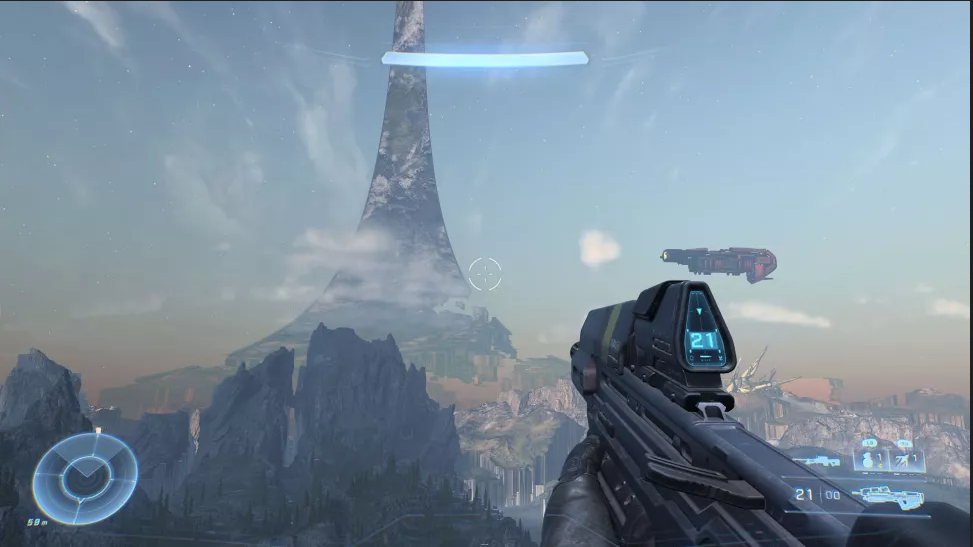
\includegraphics[scale=0.4]{pics/3d_welt_halo_ring}
    \caption{3D Welt - Halo}
    \label{fig:3d_environment_halo}
\end{figure}


%% Grafik für Destiny 2 Locations noch einbinden (Seite für Quelle lädt grade nicht Bungie.net)

\begin{figure}
    \centering
    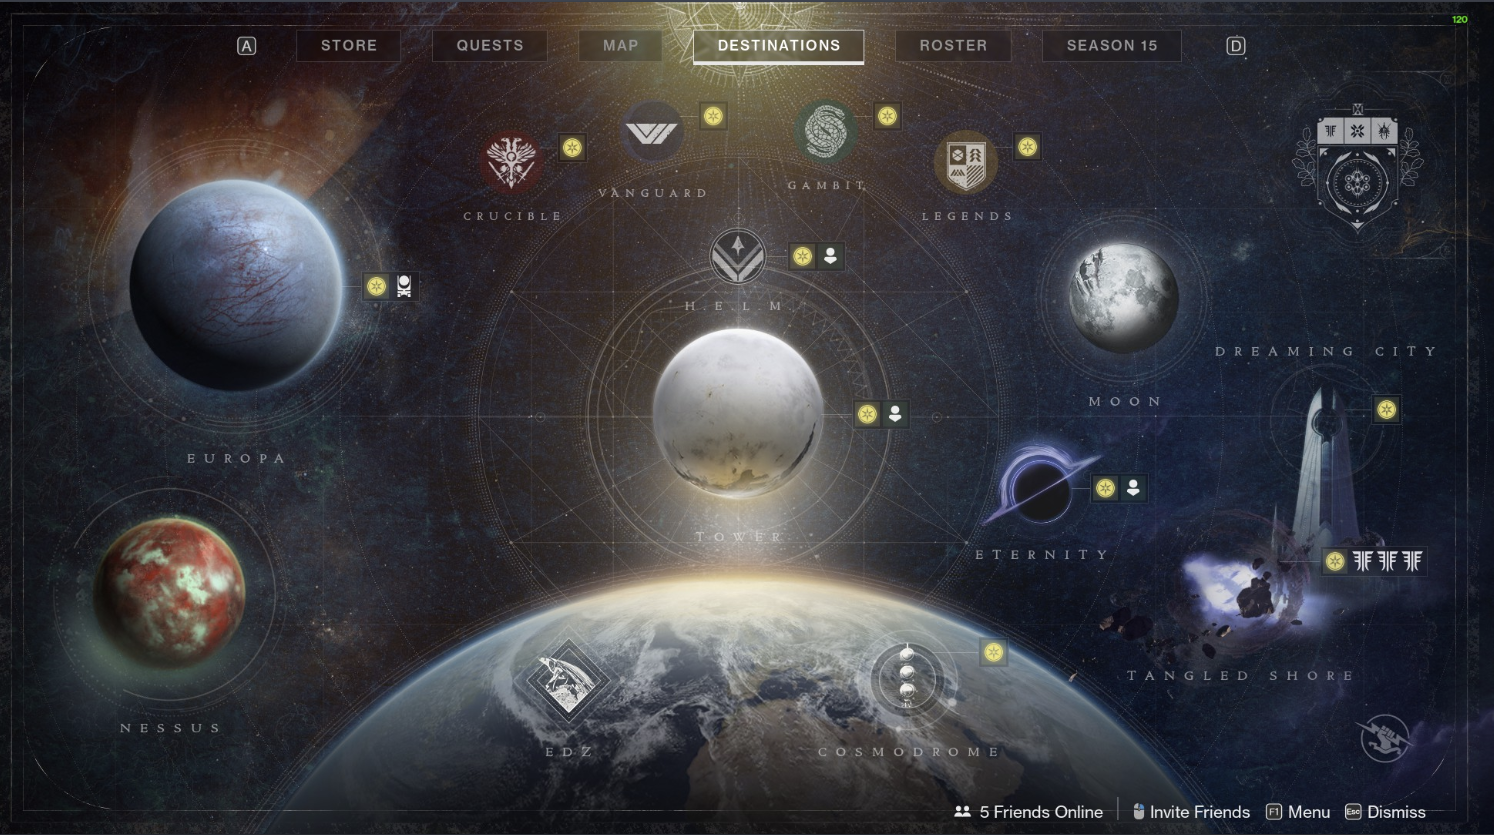
\includegraphics[scale=0.3]{pics/3d_welt_destiny_planets}
    \caption{3D Welt - Destiny 2}
    \label{fig:3d_environment_destiny2}
\end{figure}

Spielehersteller bauen die Spielwelten so auf, wie es am besten zu der Vision des Spieles passt.
Gleichzeitig wird darauf geachtet, dass sich die Umgebung nicht langweilig oder leer anfühlt.
Hierfür wird Environmental Storytelling verwendet.
Darunter versteht man das Platzieren von Gegenständen und Objekten,
welche dem Spieler eine kleine Geschichte erzählen.
Das passiert jedoch nicht über Sprache sondern einfach nur über die Platzierung und das Aussehen.
Ein Beispiel hierfür w\"are das Bild von Cayde-6 (ein Charakter aus Destiny 2), welches in einem Restaurant platziert wurde.
Cayde ist einer der drei Anführer der Vanguard, welche eine Ansammlung an Guardians (Spielern und NPC) ist und gegen das Böse kämpft.
In Forsaken starb Cayde jedoch und viele trauerten um ihn, als Gedenken wurde dieses Bild aufgehängt.
~\cite{GameDeveloper_2022}

\begin {figure}
    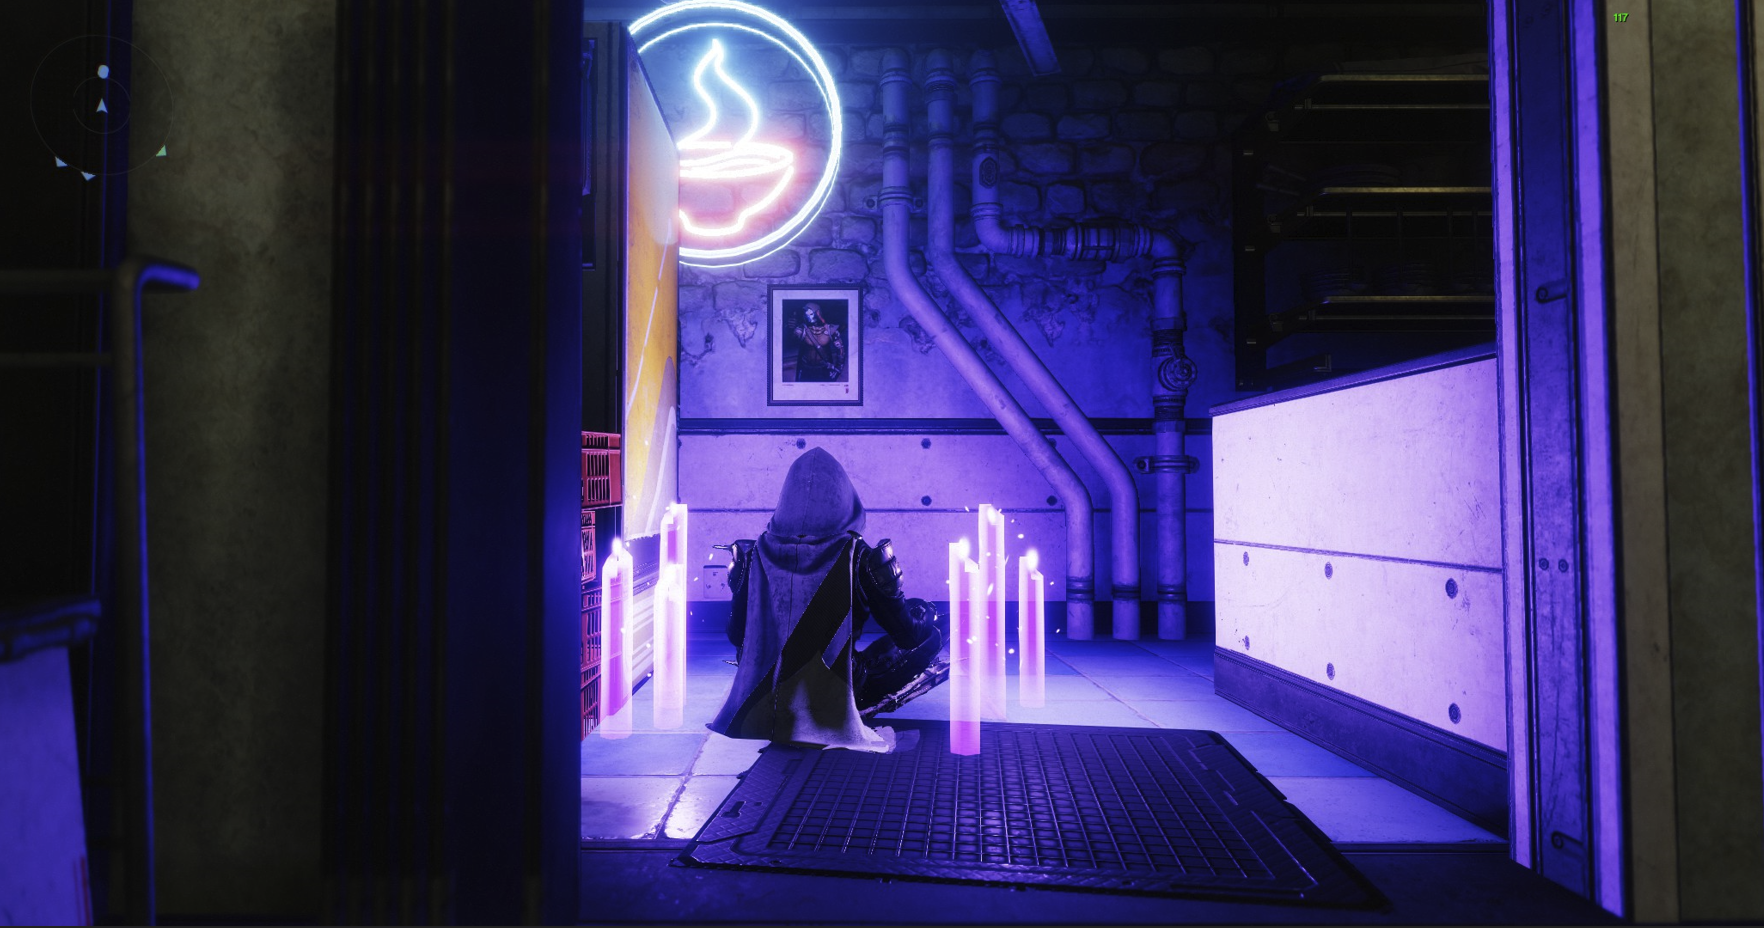
\includegraphics[scale=0.3]{pics/3d_welt_destiny2-environmental-storytelling}
    \caption{Environmental Storytelling '-' Destiny 2 Cayde}
    \label{fig:3d_environmental_storytelling_destiny2}
\end {figure}


\subsection{City Grid System}\label{subsec:city-grid-system}
\setauthor{Florian Beckerle}
Um die Gestaltung der Welt in BeamVR zu erleichtern, wurde ein Grid System verwendet.
Dafür ist die Stadt in ein Raster aufgeteilt, an welchem sich alle Objekte der Welt auf allen 3 Achsen (x,y,z) orientieren.
Unity stellt, wie in Abb. ~\ref{fig:grid-system-unity} zu sehen, so ein Grid Snapping System zur Verf\"ugung.
Daher wurde f\"ur BeamVR am Anfang der Modellierungsphase eine bestimmte Grid-Size festgelegt,
an welche die Grundfl\"achen der Geb\"aude und die Straßen
angepasst wurden.

\begin {figure}
    \centering
    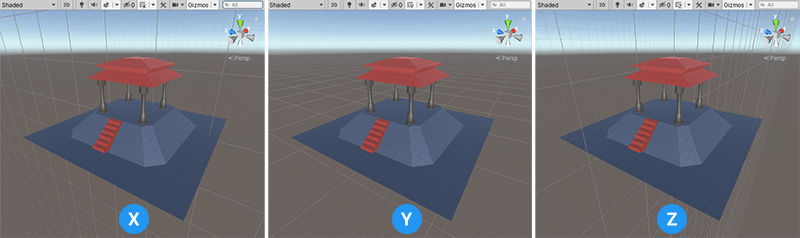
\includegraphics[scale=0.5]{pics/unity-grid-snapping}
    \caption{Unity '-' Grid Snapping System}
    \label{fig:grid-system-unity}
\end {figure}

Wenn man die Grid Size, also die Gr\"osse des Rasters \"andern m\"ochte, muss man zuerst im Editor das Grid and Snap Fenster öffnen.
Als n\"achstes findet man unter dem Bereich World Grid ein Attribut namens Size, wo man die X, Y und Z Achsen frei und unabh\"angig voneinander umskalieren kann, siehe Abb. ~\ref{fig:grid-size-unity}.
~\cite{Unity_GridSnapping_2022}

\begin {figure}
    \centering
    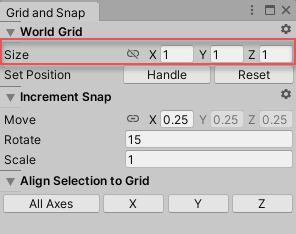
\includegraphics{pics/unity-grid-snapping-size}
    \caption{Unity - Grid Snapping Size}
    \label{fig:grid-size-unity}
\end {figure}



\subsection{Stadt}\label{subsec:city}
\setauthor{Florian Beckerle}
Jede Stadt hat viele verschiedene Strukturen wie zum Beispiel Sehensw\"urdigkeiten, Bauwerke und Einrichtungen wie Kinos, Theater oder Restaurants.
F\"ur BeamVR wurden daher insgesamt \"uber 34 Geb\"aude Modelle erstellt, um eine Vielfalt in der Umgebung zu erreichen, siehe Abb. ~\ref{fig:beamvr_building-variety}.

\begin {figure}
    \centering
    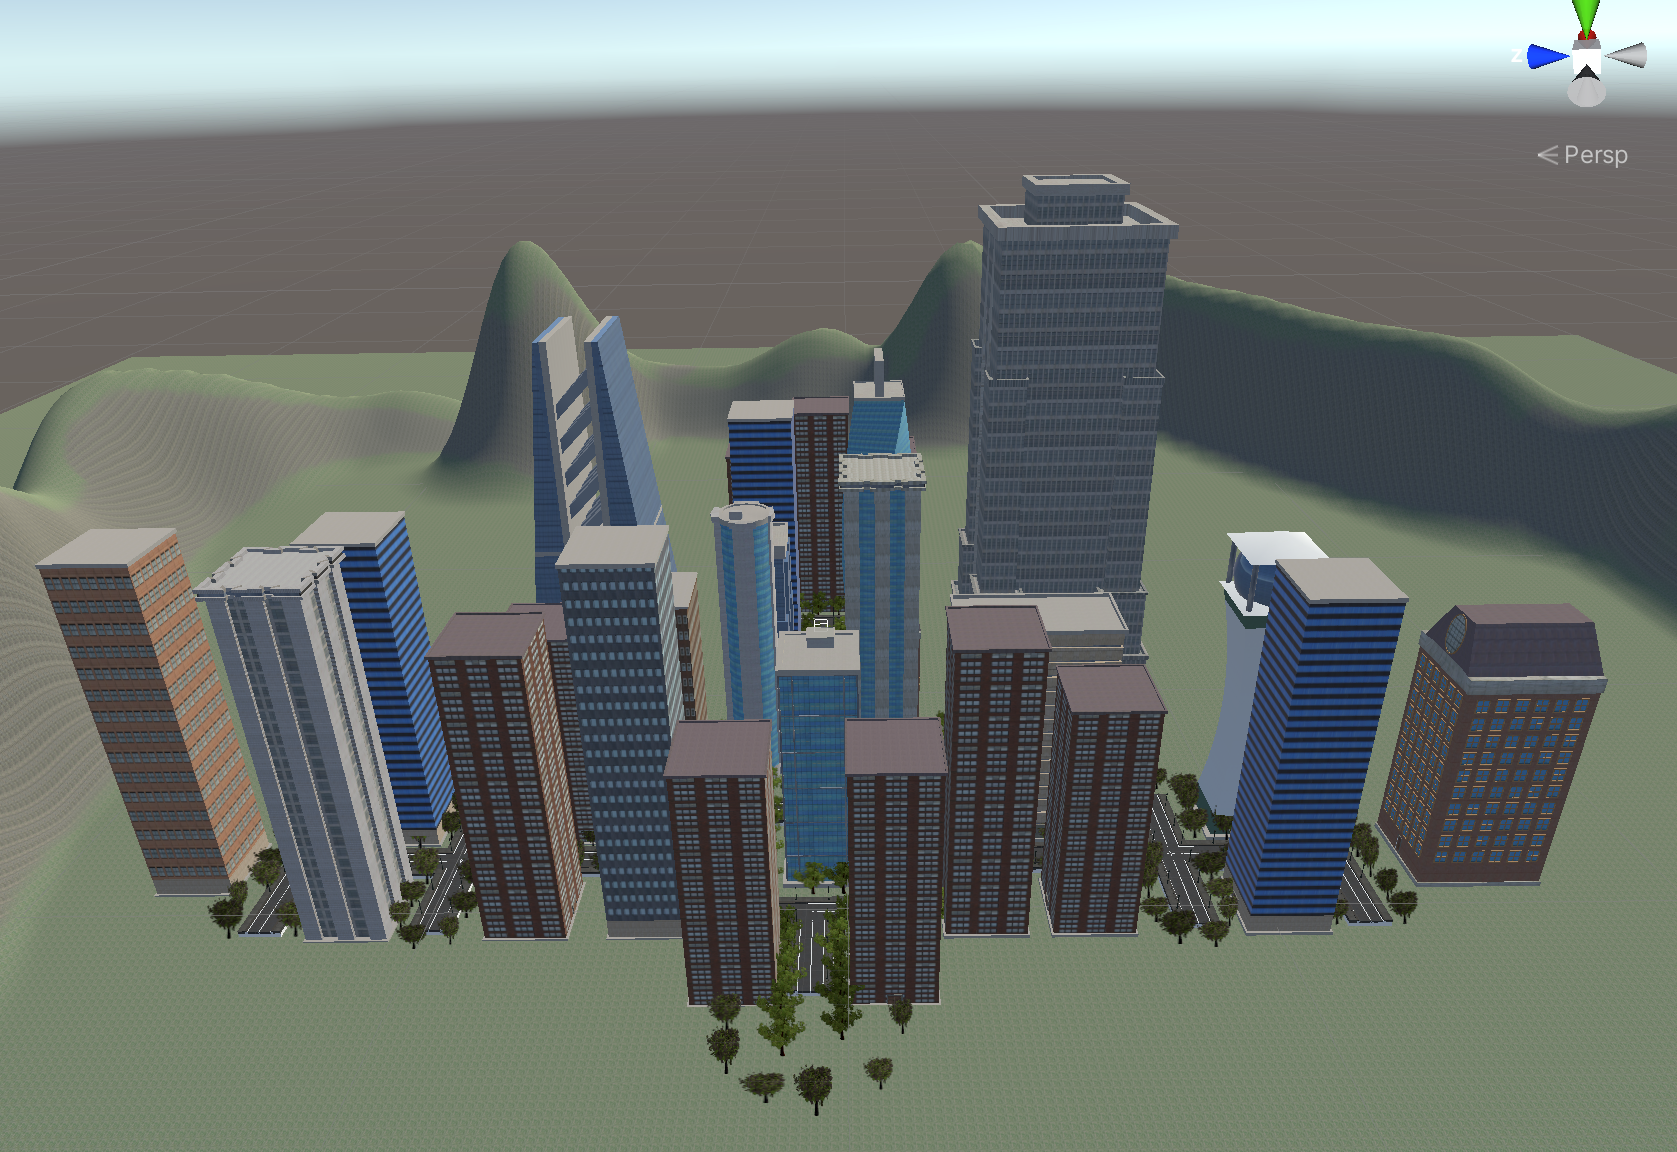
\includegraphics[scale=0.18]{pics/beamvr_building-variety}
    \caption{Beam VR - Building Overview}
    \label{fig:beamvr_building-variety}
\end {figure}

Die Stadt wurde so entworfen, dass nur die für den Spieler sichtbaren Objekte wirklich existieren, wie auf der Abb. ~\ref{fig:beamvr_building-variety} zu erkennen ist.
Bei richtiger Umsetzung scheint es für den Anwender dennoch so, als w\"are dieser in einer kompletten Spielwelt.
Um die Performance des Spieles zu verbessern, wurde dieser Trick in BeamVR angewandt, da unn\"otige Objekte nicht gerendert oder berechnet werden m\"ussen.
Bei gr\"oßeren Projekten spart das nicht nur Zeit sondern auch Ressourcen.
Bei BeamVR wurde diese Technik angewandt, um die Frames per Second zu erh\"ohen.

\subsection{Tag Stadt}\label{subsec:day-city}
\setauthor{Florian Beckerle}
Es wurden 17 der 34 unterschiedlichen Geb\"aude f\"ur diese Map modelliert, siehe Abb. ~\ref{fig:beamvr_building-variety}.
Der Fokus bei der Gestaltung der Bauwerke lag darauf, dass diese m\"oglichst realistisch aussehen und dennoch nicht zu rechenaufwendig in der Darstellung sind.
Daher wurden Texturen verwendet, um kleinere Details an den Fassaden darzustellen, statt diese zu modellieren.
Das gleiche Prinzip wurde bei der Apocalypse Map verwendet, siehe Abschnitt ~\ref{subsec:apocalypse-city}.
Die Texturen stellen Fassaden aus Stein und Glas dar.
Ein weiterer wichtiger Punkt bei der Planung der Stadt war es auch, dass der Spieler nicht aus der Stadt hinaus schauen kann und die Illusion aufrecht erhalten bleibt.
Daher wurden alle umliegenden Bauwerke mindestens 3 Meter h\"oher gemacht als das Geb\"aude, auf dem sich der Spieler befindet, siehe Abb. ~\ref{fig:beamvr_building-heights}.

\begin {figure}
    \centering
    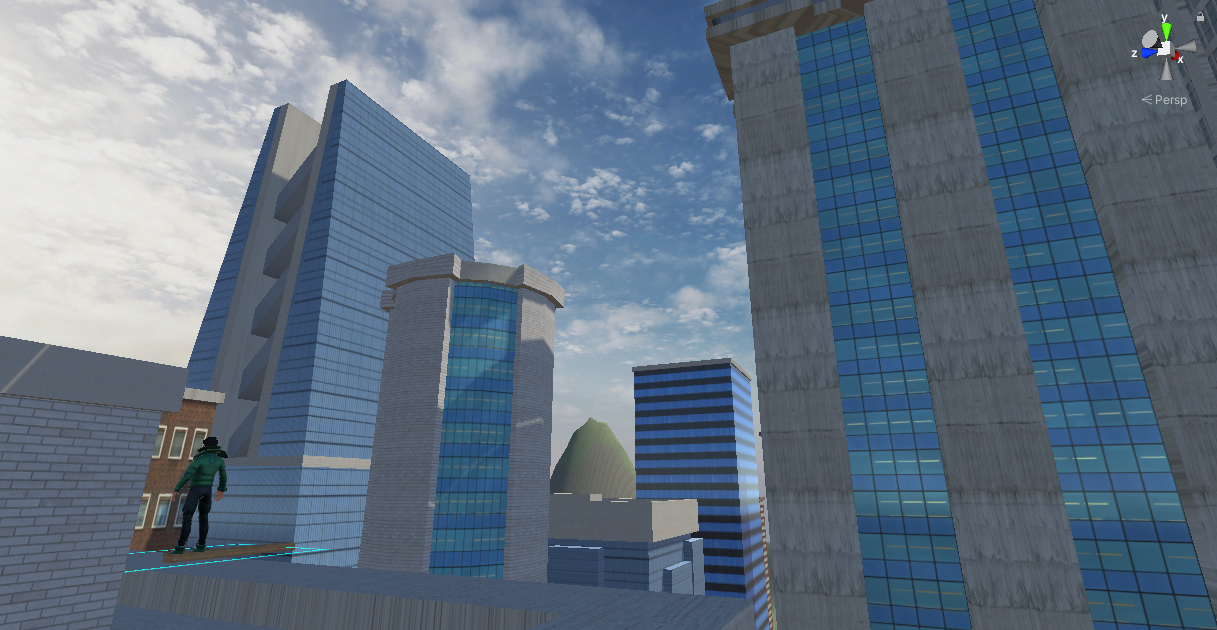
\includegraphics[scale=0.5]{pics/beamvr_city_day_heights}
    \caption{Beam VR - Building Heights}
    \label{fig:beamvr_building-heights}
\end {figure}

\subsection{Nacht Stadt}\label{subsec:night-city}
\setauthor{Florian Beckerle}
In der Nacht Version der Stadt wurde die Skybox angepasst.
Diese zeigt nun einen Sternenhimmel.
Es handelt sich hierbei um eine Sphere oder Box, welche sich um die Spielwelt befindet.
Sie wird dazu benutzt, um einen Himmel oder andere Umgebungen,
in Form von Texturen darstellen zu können, ohne dass diese als Modelle existieren.
Zus\"atzlich wurde die Belichtung der Scene auf ein bl\"auliches Licht eingestellt und die Laternen in den Straßen
haben noch eigene Lichtquellen, siehe Abb. ~\ref{fig:beamvr_night_map_lighting}.

\begin {figure}
    \centering
    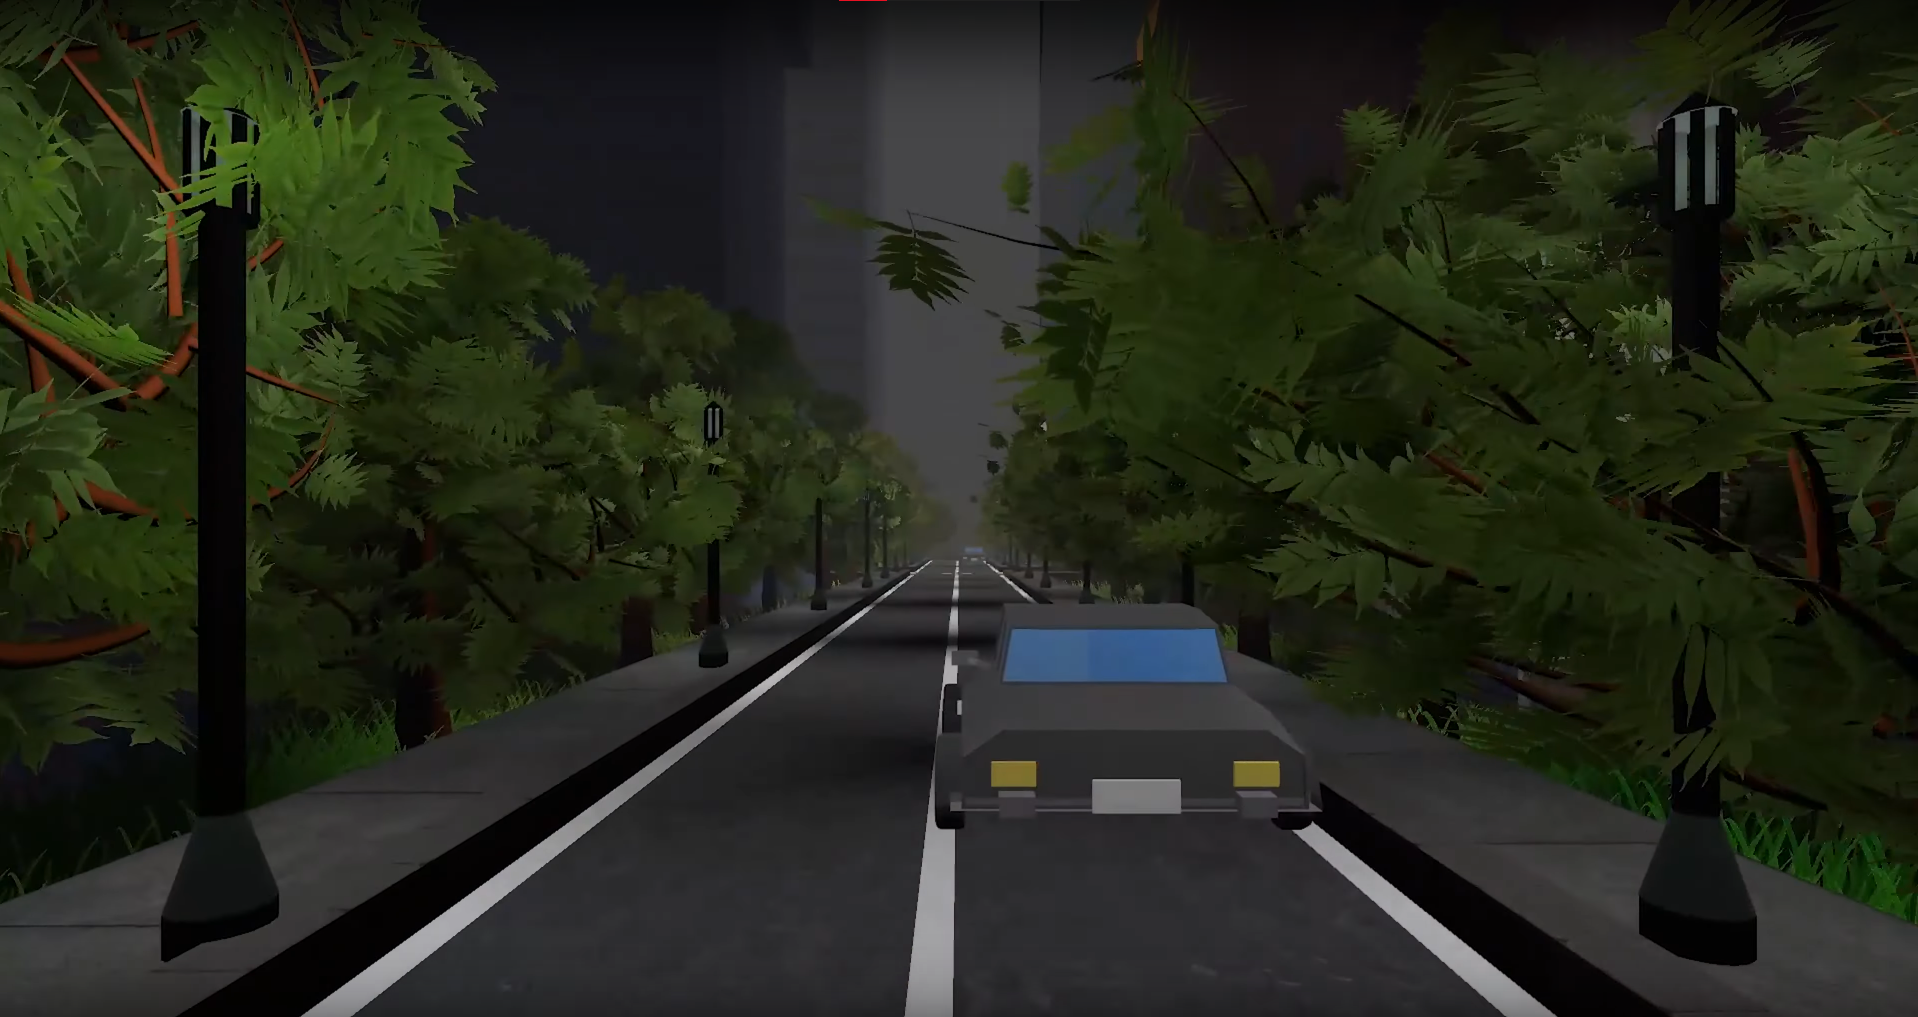
\includegraphics[scale=0.3]{pics/beamvr_night_overview}
    \caption{Beam VR - Night Map Lighting}
    \label{fig:beamvr_night_map_lighting}
\end {figure}

\subsection{Apocalypse Stadt}\label{subsec:apocalypse-city}
\setauthor{Florian Beckerle}
F\"ur diese Umgebung wurden alle Geb\"aude nocheinmal \"uberarbeitet.
Statt der intakten Glasfassaden werden nun barrikadierte Fenster und Ziegelsteine ohne Verputz f\"ur die Bauwerke verwendet, siehe Abb. ~\ref{fig:beamvr_damaged_texture}.
Durch diese \"Anderung sieht die Stadt verlassen und postapokalyptisch aus.
Um den Effekt noch zus\"atzlich zu verst\"arken, wurden die Bauwerke in eine Schieflage gebracht, sodass es aussieht, als w\"urden diese gleich zusammenbrechen.
Das Gel\"ande wurde mit neuen Sandstein Texturen und D\"unen in eine W\"uste umgewandelt.
Die Planzen und B\"aume wurden durch ausgetrocknete B\"usche ausgetauscht, damit die Welt ein trostloses Aussehen erhält, siehe Abb. ~\ref{fig:beamvr_apocalypse_map}.

\begin {figure}
    \centering
    \includegraphics{pics/beamvr_damaged_texture}
    \caption{Beam VR - Damaged Texture}
    \label{fig:beamvr_damaged_texture}
\end {figure}

\begin {figure}
    \centering
    \includegraphics[scale=0.3]{pics/beamvr_apocalypse-overview}
    \caption{Beam VR - Apocalypse Map}
    \label{fig:beamvr_apocalypse_map}
\end {figure}

\section{Sound Design}\label{sec:sound}
\setauthor{Florian Beckerle}
Ohne Sound Design würden die Maps von BeamVR unrealisitsch wirken, da in einer Stadt Lärm an der Tagesordnung steht.
In der virtuellen Umgebung der verwendeten Game Engine existieren anfangs keine Geräusche, diese m\"ussen von den Entwicklern selber erstellt und eingef\"ugt werden.


Es gibt viele verschiedene Arten Sound Design zu benutzen wie zum Beispiel die Ger\"ausche, die der Anwender selbst in der virtuellen Welt verursacht.
Wenn sich der Spieler bewegt, sollten Fußstapfen zu h\"oren sein.
Diese klingen je nach Bodentyp unterschiedlich.
Besteht der Boden aus Holz, wird man ein h\"olzernes Klopfen und Knarren h\"oren.
Ist der Boden jedoch mit Gras bedeckt, wird ein Rascheln abgespielt.
Zus\"atzlich wird der gesteuerte Charakter außer Atem sein, wenn gelaufen wurde oder gerade ein Sprung ausgef\"uhrt wird.
Das wird mithilfe von Atem-Geräuschen umgesetzt.

Bei Umgebungen ist es wichtig, dass die Welt nicht leer klingt, sondern mit situationsbedingten Hintergrundger\"auschen voller Leben erscheint.
Es gibt jedoch auch Situationen, in denen gezielt wenig Umgebungsger\"ausche benutzt werden, um zum Beispiel eine W\"uste oder eine verlassene Stadt noch einsamer und trostloser darzustellen.

Um die Stimmung noch genauer steuern zu k\"onnen, kann Musik benutzt werden.
Wenn der Spieler auf einem Pferd durch eine Weide reitet, kann eine dramatische und inspirierende Musik benutzt werden, um den Moment noch besser und cinematischer wirken zu lassen.

Die Informationen für die Absätze wurden hier gefunden ~\cite{GK_Media_Factory_Sound_Design_2022}.

\subsection{Apocalypse}\label{subsec:apocalypse-background-sound}
\setauthor{Florian Beckerle}
Die Musik in der Apocalypse Map ist stark an das Horror Genre angelegt.
Die Melodie ist jedoch nicht wirklich existent, stattdessen existiert ein durchgehendes pfeifendes Ger\"ausch, welches unterbewusst das Spannungslevel erh\"oht.
Der Spieler f\"uhlt sich etwas unbehaglich und alleine.
Dadurch wirkt die Stadt, neben den br\"ockelnden H\"ausern, zus\"atzlich noch mehr verlassen.

Da die Sicht in dieser Map stark durch einen gelblichen Nebel, der wie ein Sandsturm wirkt, eingeschr\"ankt ist, kann man im Hintergrund den Wind pfeifen h\"oren.

\subsection{City}\label{subsec:day-night-background-sound}
\setauthor{Florian Beckerle}
Die Hintergrundger\"ausche der Tag und Nacht Version der Stadt sind sehr \"ahnlich.
Der Spieler kann Motorr\"ader und Autos auf den Straßen vorbeifahren h\"oren.
Hin und wieder kann man Menschen, die man nicht sehen kann, bei kurzen Gespr\"achen miteinander zuh\"oren und ein Kind husted im Hintergrund.

\subsection{Event}\label{subsec:building-collapse-sound}
\setauthor{Florian Beckerle}
Um spezifische Events, also bestimmte Dinge, welche in der Welt passieren, f\"ur den Benutzer besser erkennbar zu machen, wurden zus\"atzlich Ge\"ausche eingef\"ugt.
Auf der Apocalypse Map sind zusammenbrechende Geb\"aude zu h\"oren, um die schlechte Instandhaltung der verlassenen Stadt erneut zu verdeutlichen.
Aber wenn der Benutzer genauer hinsieht kann man, wenn diese Sounds h\"orbar sind, auch tats\"achlich eine kleine Auswahl an Bauwerken br\"ockeln sehen.

\section{Effects}\label{sec:effects}
\setauthor{Florian Beckerle}
Unity bietet verschiedene M\"oglichkeiten, um das Aussehen der Applikation zu beeinflussen.
Mithilfe von Post Processing kann man Effekte zu dem Buffer der Kamera, also dem aktuellen Frame, der gerade aufgenommen wurde, hinzuf\"ugen bevor etwas am Bildschirm angezeigt wird.
Eine kleine Auswahl dieser Effekte sind zum Beispiel Bloom, Grain oder Color Grading.
~\cite{Unity_Post_Processing_2022}

Post Processing kann global angewandt werden, somit werden die eingestellten Effekte \"uber die komplette Spielwelt angezeigt.
Um die Effekte auf einen bestimmten Bereich zu begrenzen, muss ein Collider erstellt und platziert werden.
Wenn die Kamera in diesem Collider ist, wird das angezeigte Bild mit den eingetellten Effekten versehen.
~\cite{Unity_Post_Processing_Volumes_2022}

Der Bloom Effekt wird dazu benutzt, um sehr helle Stellen und Objekte, wie bei einer echten Kamera, ausgebrannt darstellen zu können.
Hierbei wirkt das Objekt etwas verschwommen und durch die Helligkeit ist kaum etwas zu erkennen, siehe Abb. ~\ref{fig:unity-post-processing-bloom}.
\begin {figure}
    \centering
    \includegraphics[scale=0.9]{pics/unity-post-processing-bloom}
    \caption{Unity - Post Processing Bloom}
    \label{fig:unity-post-processing-bloom}
\end {figure}
Dieser Effekt kann mithilfe von verschiedenen Parametern angepasst werden.
Die Intensität steuert die Stärke des Effektes, also wie stark das Bild verändert wird.
Der Treshhold filtert alle Pixel, welche unter einem bestimmten Helligkeitsniveau liegen, heraus.
Diese Pixel sind nicht von den Änderungen betroffen.
Wenn Soft Knee auf 1 gestellt wird, ist der Übergang zwischen Pixeln, die durch den Treshhold gefiltert werden, weicher.
Bei 0 befindet sich die Grenze genau auf dem eingestellten Wert.
Der Radius beeinflusst die Ausbreitung des Blooms von einem hellen Objekt aus.
Es kann zusätzlich ein Lens Dirt Effekt angewandt werden, hierbei entstehen Flecken in den hellen Bereichen, siehe Abb. ~\ref{fig:unity-post-processing-lens-dirt}.
~\cite{Unity_Post_Processing_Bloom_2022}

\begin {figure}
    \centering
    \includegraphics[scale=0.9]{pics/unity-post-processing-lens-dirt}
    \caption{Unity - Post Processing Lens Dirt}
    \label{fig:unity-post-processing-lens-dirt}
\end {figure}

Grain fügt dem angezeigten Bild einen Noise Effekt hinzu.
Hierfür wird ein nahtloses Rauschen angewandt, welches Unvollkommenheiten von Filmbändern ähnelt, siehe Abb. ~\ref{fig:unity-post-processing-grain}.
\begin {figure}
    \centering
    \includegraphics[scale=0.9]{pics/unity-post-processing-grain-on}
    \caption{Unity - Post Processing Grain}
    \label{fig:unity-post-processing-grain}
\end {figure}
Dieser Effekt kann ebenfalls mithilfe von verschiedenen Attributen verändert werden, siehe Abb. ~\ref{fig:unity-post-processing-grain-ui}.
Intensity steuert die Sichtbarkeit des Rauschens im Bild.
Luminance Contribution steuert das Rauschen abhängig von der Helligkeit einer Stelle im Bild.
Bei einem niedrigen Wert ist in dunklen Gebieten kaum Rauschen zu sehen.
Die Größe der Partikel wird vom Size Parameter gesteuert.
\begin {figure}
    \centering
    \includegraphics[scale=0.9]{pics/unity-post-processing-grain-ui}
    \caption{Unity - Post Processing Grain UI}
    \label{fig:unity-post-processing-grain-ui}
\end {figure}
~\cite{Unity_Post_Processing_Grain_2022}

Color Grading wird für die Korrektur von Farben und Helligkeit, eines Bildes verwendet.
Ein Beispiel für die Auswirkungen dieses Effekts sieht man in Abbildung ~\ref{fig:unity-post-processing-color-grading-example}.
Der linke Teil des Bildes wurde bearbeitet, der rechte Teil zeigt die ursprünglichen Farben des Bildes an.
Der linke Teil des Bildes wurde bearbeitet, der rechte Teil zeigt die ursprünglichen Farben des Bildes an.
Color Grading hat 5 verschiedene Sektionen, mit welchen genauere Einstellungen getroffen werden können.
Darunter fallen Tonemapping, Basic, Channel Mixer, Trackballs und Grading Curves.
~\cite{Unity_Post_Processing_ColorGrading_2022}
\begin {figure}
    \centering
    \includegraphics[scale=0.4]{pics/unity-post-processing-color-grading-before-after}
    \caption{Unity - Post Processing Color Grading Example}
    \label{fig:unity-post-processing-color-grading-example}
\end {figure}

Tonemapping beschreibt den Prozess, in welchem HDR Werte eines Bildes so umgewandelt werden, um auf einem Bildschirm dargestellt werden zu können.
Es werden dabei drei Modes zur Verfügung gestellt.
Der Neutral Tonemaper wandelt die Werte, mit möglichst geringem Einfluss auf Farbe und Sättigung, um und verwendet eine Tonemapping Curve, siehe Abb. ~\ref{fig:unity-post-processing-neutral-tonemapper-ui}.
Black In und White In steuern dabei die inneren weißen und schwarzen Kontrolpunkte, Black Out und White Out steuern die äußeren Punkte.
%Mit dem White Level kann auf einen weißen Punkt vor der Kurve eingestellt werden.
White Clip stellt auf einen weißen Punkt nach der Kurve ein.
\begin {figure}
    \centering
    \includegraphics[scale=0.9]{pics/unity-post-processing-color-grading-neutralTonemapper}
    \caption{Unity - Post Processing Neutral Tonemapper UI}
    \label{fig:unity-post-processing-neutral-tonemapper-ui}
\end {figure}

Der Filmic (ACES) Tonemapper verwendet Schätzwerte  des ACES Tonemappers, um ein filmisches Aussehen zu erreichen.
Das Resultat ist ein höherer Kontrast und es wird Einfluss auf die Farbe und Sättigung des Bildes genommen.
Dieser Tonemapper besitzt keine Einstellungsmöglichkeiten, siehe Abb. ~\ref{fig:unity-post-processing-filmic-aces-tonemapper-ui}.

\begin {figure}
    \centering
    \includegraphics[scale=0.9]{pics/unity-post-processing-color-grading-filmic}
    \caption{Unity - Post Processing Filmic (ACES) Tonemapper UI}
    \label{fig:unity-post-processing-filmic-aces-tonemapper-ui}
\end {figure}

Der Basic Tonemapper stellt simple Einstellungsmöglichkeiten zur Verfügung und ist ein empfohlener Startpunkt für Farbkorrekturen.
Es können Einstellungen wie Post Exposure, Temperature, Tint, Hue Shift, Staturation und Contrast eingestellt werden, siehe Abb. ~\ref{fig:unity-post-processing-basic-tonemapper-ui}.
\begin {figure}
    \centering
    \includegraphics[scale=0.9]{pics/unity-post-processing-color-grading-basicTonemapper}
    \caption{Unity - Post Processing Basic Tonemapper UI}
    \label{fig:unity-post-processing-basic-tonemapper-ui}
\end {figure}

Post Exposure stellt die allgemeine Belichtung der Scene in EV Einheiten dar.
Dieser Effekt wird erst nach den HDR Effekten, aber vor dem Tonemapping, eingesetzt, damit die vorherigen Effekte nicht beeinflusst werden.
Die Temperatur setzt die White Balance zu einer beliebig eingestellten Farbtemperatur.
Mithilfe von Tint kann ein grüner oder magenta Tint im Bild korrigiert werden.
Hue Shift verschiebt das HUE aller Farben, während Saturation die Intensität dieser beeinflusst.
Der Contrast erweitert oder verkleinert die Breite zwischen den dargestellten Farben.

Mithilfe des Channel Mixers kann der Einfluss der einzelnen Farbkanäle, welche Rot, Grün und Blau sind, auf das gesamte Bild eingestellt werden.
Wie in Abb. ~\ref{fig:unity-post-processing-channel-mixer-ui} zu sehen ist, kann dabei jeder Farbkanal einzeln mittels eines Schiebereglers verändert werden.
Ein Beispiel für die Auswirkungen dieses Effekts ist in Abb. ~\ref{fig:unity-post-processing-channel-mixer} zu erkennen.
\begin {figure}
    \centering
    \includegraphics[scale=0.9]{pics/unity-post-processing-channel-mixer-ui}
    \caption{Unity - Post Processing Channel Mixer UI}
    \label{fig:unity-post-processing-channel-mixer-ui}
\end {figure}

\begin {figure}
    \centering
    \includegraphics[scale=0.4]{pics/unity-post-processing-channel-mixer-example}
    \caption{Unity - Post Processing Channel Mixer}
    \label{fig:unity-post-processing-channel-mixer}
\end {figure}

Mithilfe von Trackballs kann man ein 3-Wege Color Grading in einem Linearen oder Logarithmischen System vornehmen.
Bei der Logarithmus Variante werden die Farbverteilung und der Contrast komprimiert um einen Color-Timing Process, welcher von optischen Film Druckern erzeugt wird, zu simulieren, siehe Abb. ~\ref{fig:unity-post-processing-trackballs-log}.
Hierbei kann mit Power das Gamma und mit Offset das Signal beeinflusst werden.
\begin {figure}
    \centering
    \includegraphics[scale=0.9]{pics/unity-post-processing-trackballs-log}
    \caption{Unity - Post Processing Trackballs Log}
    \label{fig:unity-post-processing-trackballs-log}
\end {figure}
Die Lineare Methode wurde für linear-encododed Data optimiert, siehe Abb. ~\ref{fig:unity-post-processing-trackballs-linear} für das UI.
Mithilfe von Lift kann das gesamte Signal verschoben werden.
Gamma beeinflusst wieder die mittleren Töne und Gain verstärkt das Signal.
\begin {figure}
    \centering
    \includegraphics[scale=0.9]{pics/unity-post-processing-trackballs-linear}
    \caption{Unity - Post Processing Trackballs Linear}
    \label{fig:unity-post-processing-trackballs-linear}
\end {figure}

Mithilfe von fünf verschiedenen Grading Curves können YRGB, Hue vs Hue, Hue vs Sat, Sat vs Sat und Lum vs Sat verändert werden.
Hierbei handelt es sich jedesmal um eine Kurvendarstellung, in welcher man weitere Punkte setzen und damit den Verlauf der Kurve beeinflussen kann, siehe Abb. ~\ref{fig:unity-post-processing-grading-curve-example}.
\begin {figure}
    \centering
    \includegraphics[scale=0.9]{pics/unity-post-processing-grading-curve-example}
    \caption{Unity - Post Processing Grading Curve Example}
    \label{fig:unity-post-processing-grading-curve-example}
\end {figure}
Bei der YRGB Kurve kann durch die Manipulation des Graphen der Contrast und die Helligkeit des Bildes eingestellt werden.
Die Hue vs Hue Kurve bietet die Möglichkeit, Farbbereiche zu verfeinern oder auszutauschen.
Um eine bestimmte Farbe besonders hervorzuheben oder einen monochromatischen Effekt zu erreichen, wird die Hue vs Sat Kurve verwendet.
Bei der Sat vs Sat Kurve werden einfache Veränderungen der Farbe wie beim Color Grading vorgenommen.
Die letzte Option heißt Lum vs Sat Kurve und ermöglicht es, in bestimmten Gebieten die Sättigung zu verringern, wie zum Beispiel in dunklen Stellen.

\subsection{Nebel}\label{subsec:fog-effect}
\setauthor{Florian Beckerle}
Unity bietet mehrere M\"oglichkeiten, Nebel darzustellen, zum Beispiel mittels Post Processing, oder mithilfe der Lighting Einstellungen.
F\"ur BeamVR wurde die zweite Variante verwendet, da der Nebel in BeamVR kein Hauptaugenmerk ist und mithilfe dieser Methode das Einstellen für BeamVR schneller ging.
~\cite{Unity_Lighting_Window_2022}

Mittels Post Processing wird ein Screen-Space Nebel Effekt in der Tiefen-Texture der Kamera erstellt, siehe Abb. ~\ref{fig:unity_post_processing_fog}.
Screen-Space bedeutet, dass die Position auf dem Bildschirm und nicht in der dreidimensionalen Welt berechnet wird.
~\cite{Unity_Fog_2022}

\begin {figure}
    \centering
    \includegraphics[scale=0.9]{pics/unity-post-processing-fog}
    \caption{Unity - Post Processing Fog}
    \label{fig:unity_post_processing_fog}
\end {figure}
Unter dem Begriff Map versteht man eine Umgebung in einer Spielwelt, in diesem Fall wird auf die Szenen, in welchen die Städte platziert sind, verwiesen.
Auf fast jeder Map von BeamVR wurde dieser Nebel verwendet.
In der Nacht Map wird mithilfe dieses Effekts ein leichter Nebel dargestellt, was zur abendlichen Stimmung beitr\"agt.
Bei Apocalypse ist der Nebel viel dichter und stellt einen Sandsturm dar. Zus\"atzlich wurde dieser gelb gef\"arbt, um noch mehr an Sand zu erinnern, siehe Abb. ~\ref{fig:beamvr_yellow_fog}.

\begin {figure}
    \centering
    \includegraphics[scale=0.3]{pics/beamvr_yellow_fog}
    \caption{Beam VR - Yellow Fog}
    \label{fig:beamvr_yellow_fog}
\end {figure}

Mittels der High Definition Render Pipeline, welche auch als HDRP bezeichnet wird, kann ebenfalls Nebel eingestellt werden.
Hierfür wird die Volume Framework benötigt, in welcher ein Nebel Overrride hinzugefügt wird.

Diese Framework bietet einige verschiedene Optionen zur Beeinflussung des Nebels, siehe Abb. ~\ref{fig:unity-hdrp-fog}.
Die Option Enable wird verwendet, um den Effekt zu aktivieren oder deaktivieren.
Die Fog Attenuation Distance bestimmt die Dichte und die Sichtweite im Nebel.
Ab der eingestellten Distanz hat der Nebel bereits 63\% des Umgebungslichts absorbiert.
Dichte und Sichtweite bleiben bis zu einer definierten Base Height constant, erst ab dieser ist eine exponentielle Abnahme beider Attribute erkennbar.
Die Maximum Height und Max Fog Distance bestimmen die Stärke des Abfalls und die Distanz des Nebels.
Mittels des Color Modes kann die Farbe des Nebels beeinflusst werden.
Bei Sky Color wird die Farbe automatisch an den Himmel angepasst, während bei constant Color eine eigene Farbe eingestellt werden kann.

Volumetric Fog kann mittels der gleichnamigen Option aktiviert werden.
Die Albedo Option setzt dabei die Farbe des Nebels, mit welcher das Licht gestreut wird.
Lichter werden, mit zunehmender Dichte des Nebels, schneller abgedunkelt.
Anisotropy steuert die Streuung des Lichtes.
0 streut das Licht gar nicht, 1 streut das Licht vorwärts und -1 streut rückwärts.
Mittels eines Filters kann eine Unschärfe der eingehenden Lichter geschaffen werden, damit ein weicherer Übergang zustande kommt.
~\cite{Unity_HDRP_Fog_2022}

\begin {figure}
    \centering
    \includegraphics[scale=0.9]{pics/unity-hdrp-fog}
    \caption{Unity - HDRP Fog}
    \label{fig:unity-hdrp-fog}
\end {figure}


\subsection{Lichter}\label{subsec:light-effect}
\setauthor{Florian Beckerle}
In der Nacht Map wurden die von Unity bereitgestellten Point-Lights als Straßenlichter benutzt.
Point Lights k\"onnen mithilfe eines Radius auf einen bestimmten kreisf\"ormigen Bereich eingegrenzt werden.
Weiters wird mithilfe der Lichtst\"arke die Wirkkraft des Lichtes in diesem Gebiet genauer bestimmt.
Dank dieser Eigenschaften war das Point Light f\"ur die Aufhellung der Straßen, siehe Abb. ~\ref{fig:beamvr_street_lights}.
~\cite{Unity_PointLights_2022}
\begin {figure}
    \centering
    \includegraphics[scale=0.3]{pics/beamvr_point_lights}
    \caption{Beam VR - Street Lights}
    \label{fig:beamvr_street_lights}
\end {figure}

\subsection{Wind}\label{subsec:wind-effect}
Damit sich die B\"aume und B\"usche in BeamVR wie im Wind bewegen, werden Unitys Wind Zones ben\"otigt.
Diese Zonen sind bestimmte Bereiche, in welchen eine Windrichtung, Windst\"arke und Turbulenz definiert wird.
Die eingestellten Effekte werden dann auf alle Objekte angewandt, die mithilfe des Terrains oder Particle Systems iniziiert wurden.
~\cite{Unity_WindZones_2022}

\section{Unity Prefabs}
\label{sec:prefabs}
\setauthor{Quirin Ecker}

In Unity gibt es ein System welches dem Entwickler oder der Entwicklerin erlaubt eine bestimmte Zusammenstellung von 3d Elementen zu speichern und mehrmals in verschiedenen Szenen zu verwenden.
Diese Zusammenstellungen von 3d Elementen heißen auch Prefabs.
Wird dieses Prefab verändert, wird es an jeder platzierten Stelle aktualisiert.
Es werden dabei die Komponenten und Positionen der einzelnen Elemente relativ zu dem Prefab gespeichert.

Prefabs können auch überschrieben werden an der Stelle wo sie platziert worden sind.
Aus Erfahrung zeigt sich aber, dass dies mit Vorsicht zu genießen ist, da lokale Änderungen nicht mehr global überschrieben werden.
Somit haben globale Änderungen keinen wirklichen Einfluss auf das lokale Prefab.
Außerdem können Prefabs auch ineinander verschachtelt werden~\cite{Unity_Prefabs}.

In der BeamVR Applikation wird dieses System an mehreren Stellen verwendet.
Diese Prefabs wurden beispielsweise in der BeamVR Applikation für einzelne Elemente, welche in allen Karten existieren, benutzt.
Alle diese Elemente werden in ein sogenanntes Game Prefab gruppiert, welches in allen Karten platziert wird.

Folgend werden das Game Prefab und zwei weitere für BeamVR relevante Prefabs noch genauer beschrieben.

\subsection{Game}\label{subsec:game-prefab}

Wie bereits beschrieben befinden sich alle Game relevant Elemente in dem Game Prefab.
Somit wird dieses Prefab in allen Karten Szenen verwendet.
Nur in der Menü- und Setup-Szenen wird dieses Prefab nicht gebraucht.

Folgend sind die wichtigsten Elemente des Game Prefab aufgelistet:

\begin{itemize}
    \item \textbf{Beam:} Der Beam ist der virtuelle Balken, der von dem Hochhaus absteht.
    \item \textbf{Collider:} Die Collider sind Elemente, welche Aktionen auslösen, wenn ein anderes Element mit diesen kollidiert.
    Visuelle sind diese Collider unsichtbar.
    \item \textbf{GameCameraRig:} Das~\emph{GameCameraRig} ist ein weiteres Prefab, welches für VR spezifische Elemente zuständig ist.
\end{itemize}


\subsection{GameCameraRig}\label{subsec:game-camera-rig}

Wie bereits im Game Prefab beschrieben ist das GameCameraRig Prefab ein bestandteil des Game Prefab und beinhaltet alle VR spezifischen Elemente.
Dieses Prefab ist ein abgeändertes CameraRig Prefab, welches bereits von dem SteamVR Plugin zur Verfügung gestellt worden ist.
Das Prefab an sich soll den VR Raum darstellen.

Folgende sind die wichtigsten Elemente des GameCameraRig Prefab aufgelistet:

\begin{itemize}
    \item \textbf{Controller:} Die Controller sind Elemente welche eine SteamVR Controller Script-Component beinhalten.
    Durch dieses Script befindet sich dieses Element in der richtigen Position und Orientierung relativ zu der VR Fläche.
    \item \textbf{Camera:} Genauso wie die Controller Elemente besitzt das Camera Element auch ein Script.
    Mit diesem Script nimmt die Kamera die Position und Orientierung des Headsets relativ zur VR Fläche an.
    Diese Kamera ist auch für die Sicht des Spielers zuständig.
    \item \textbf{Tracker Objekte} Diese Elemente haben ebenfalls wieder ein ähnliches Script.
    Durch dieses Script befindet sich dieses Element in der gleichen Position und Orientierung des physischen Tracker.
    In der Script Komponente kann in einem Auswahlmenü der richtige Tracker eingestellt werden.
    \item \textbf{Spieler Modell:} Das Spieler Modell ist das Modell, welches nach dem Kalibrieren des Full-Body-Trackings die Pose des Spielers einnimmt.
    \item \textbf{VRIK Calibration Controller:} Bei diesem Element befindet sich ein Script-Component, in dem das Full-Body-Tracking konfiguriert werden kann.
    Für mehr Informationen wird auf Abschnitt~\ref{sec:final-ik-plugin} verwiesen.
\end{itemize}

\subsection{MenuCameraRig}\label{subsec:menu-camera-rig}

Das MenuCameraRig ist genauso wie das GameCameraRig eine Abänderung des von SteamVR Plugin bereitgestellte CameraRig.
Im Gegensatz zum GameCameraRig wird das MenuCameraRig nicht in den 3 Karten verwendet.
Das MenuCameraRig wird in den Menü-Szenen verwendet und besteht aus Menü und VR spezifische Elemente.

Viele Elemente sind gleich wie bei dem GameCameraRig.
Der große Unterschied des MenuCameraRig ist, dass die Controller noch weitere Script-Componenten beinhalten.
Diese sind Input Scripts welche für den Auswahlstrahl und das Auswählen der Menü-Elemente verantwortlich sind.

%TODO: (Quirin Ecker)(optional) Möglichkeit für ein Bild eines Inputstrahls

Weiters sind viele der game-spezifischen Elemente in diesem Prefab nicht vorhanden.
Beispielsweise gibt es keine Full-Body-Tracking Elemente, wie das Spieler-Modell und der VRIK-Calibration-Controller.


\begin{spacing}{1}
	\chapter{Inbetriebnahme}\label{ch:commisioning}
\end{spacing}
\setauthor{Quirin Ecker}

Die BeamVR Applikation benötigt viele Geräte und Gegenstände um die Immersion zu gewährleisten.
Daher sind sehr viele Schritte involviert, um BeamVR in ihrer vollen Funktionalität zu genießen.
Folgende Schritte sind involviert:

\begin{itemize}
    \item Aufbau
    \item Steam VR Installation
    \item VR Headset Verbindung
    \item Tracker Verbindung
    \item Steam VR Setup
    \item Applikation Starten
    \item Beam Kalibration
    \item Full Body Tracking Kalibration
\end{itemize}


\section{Aufbau}\label{sec:aufbau}

Folgend werden alle Gegenstände und Geräte für den Aufbau in Abb.~\ref{fig:assembly} aufgelistet.

\begin{figure}
    \centering
    \includegraphics[scale=0.5]{pics/assemlbly}
    \caption{Aufbau}
    \label{fig:assembly}
\end{figure}

\begin{enumerate}
    \item VR Raum
    \item Lighthouses~\ref{sec:lighthouse_tracking}
    \item Monitor
    \item Balken
    \item Startposition
    \item Virtueller Abgrund
\end{enumerate}

\subsection{Erklärung}\label{subsec:description}

Die folgende Erklärung bezieht sich dabei auf die Abbildung~\ref{fig:assembly}
Der Spieler oder die Spielerin startet bei der Startposition und balanciert entlang des Balkens.
Die Base-Stations müssen diagonal zueinander positioniert werden.
Für mehr Information über die Base-Stations wird auf den Abschnitt~\ref{sec:lighthouse_tracking} verwiesen.
Der Balken sollte ca in der Mitte positioniert werden und die langen seiten sollten möglichst parallel zu den langen seiten des VR Raums sein.

Leichte Abweichungen der optimalen position sind nicht problematisch.
Größere Abweichungen können zu unerwarteten Verhalten führen.
Die echte Position des Monitors muss nicht in der gleichen Position wie in der Abbildung sein.
Dabei ist die Kennzeichnung nur für die Kalibrierung wichtig.

\section{Steam VR Installation}\label{sec:steam-vr-installation}

\begin{figure}
    \centering
    \includegraphics[scale=0.4]{pics/steam-vr-in-store}
    \caption{Steam VR Download}
    \label{fig:steam-vr-in-store}
\end{figure}

Offiziell werden die Valve Index und die HTC Brillen von BeamVR unterstützt.
Somit funktioniert die Applikation mit SteamVR.
Steam VR ist eine Software welche auf Steam herunterladbar ist.
Es ist dabei nicht wichtig, dass die SteamVR Installation vor dem Einstecken der Geräte erfolgt.
Der Download für die Software ist in dem Steam Store zu finden.
In Abb.~\ref{fig:steam-vr-in-store} ist ein Screenshot von der Steam VR Downloadseite zu sehen.

\section{VR Headset Verbindung}\label{sec:vr-headset-verbindung}

Die Verbindung von dem Headset zu dem Computer ist von Headset zu Headset unterschiedlich.
Deshalb wird in Zuge diesr Arbeit nur die Verbindung mit einer HTC Vive Pro beschrieben.
Dabei ist auch die kabellose Variante inkludiert, welche mit dem HTC Vive Wireless Adapter funktioniert.
Für mehr informationen zu dem Adapter wird auf~\ref{subsec:wireless-virtual-reality} verwiesen.

\subsection{Tethered}\label{subsec:tethered}

\begin{figure}
    \centering
    \includegraphics[scale=0.4]{pics/link-box-setup}
    \caption{Aufgesetzte Linkbox}
    \label{fig:link-box-setup}
\end{figure}


In der Box der HTC Vive Pro befindet sich eine sogenannte Linkbox.
Diese Linkbox ist die Zentralstelle, an der das Headset steckt, die Kabel zu dem Computer und das Stromkabel.
Diese Ports sind auf zwei Seiten aufgeteilt.
Eine Seite ist nur für das Headset Kabel und die andere Seite ist für den Strom und die PC-Verbindung.
Das Headset Kabel ist ein spezielles Kabel für die Brille, das Stromkabel ein Power-Adapter und die PC-Verbindung ist ein USB-A Kabel und ein Mini Displayport zu normalen Displayport Kabel~\cite{VivePro_Setup}.
In Abb.~\ref{fig:link-box-setup} ist eine aufgesetzte Linkbox zu sehen.
Für mehr Informationen wird auf~\cite{VivePro_Setup} verwiesen.

\subsection{Wireless Adapter}\label{subsec:wireless-adapter}

Mit dem Wireless Adapter kann das Headset ohne Kabel verwendet werden.
Das Aufsetzen von dem Wireless Adapter ist etwas komplizierter.
Wie bereits in dem Abschnitt~\ref{subsec:wireless-virtual-reality} braucht diese Verbindung zu dem Computer auch eine Linkbox.

\begin{figure}
    \centering
    \includegraphics[scale=0.5]{pics/vive-wireless-setup-linkbox}
    \caption{Linkbox Setup~\cite{Wireless_Adapter_Setup_Docs}}
    \label{fig:vive-wireless-setup-linkbox}
\end{figure}


In diesem Fall reicht ein Kabel, welches diese Linkbox verbindet.
Dieses Kabel ist dann mit einer PCIe Karte im Computer verbunden, welche vor diesem Prozess in den Computer eingebaut werden muss.
Die Linkbox an sich muss statisch irgendwo positioniert werden.
Mögliche Orte dafür wären das der Monitor oder die Wand.
Grundsätzlich wäre es optimal, dass die Linkbox eine freie Sicht auf die VR-Brille hat~\cite{Wireless_Adapter_Setup_Docs}.
In Abb.~\ref{fig:vive-wireless-setup-linkbox} ist auf dem Monitor eine mit dem links stehenden PC verbundene Linkbox.

\begin{figure}
    \centering
    \includegraphics[scale=0.3]{pics/vive-wireless-setup-adapter}
    \caption{Angesteckter Adapter~\cite{Wireless_Adapter_Setup_Page}}
    \label{fig:vive-wireless-setup-adapter}
\end{figure}


Schlussendlich wird für das kabellose Erlebnis noch der Adapter gebraucht, welcher auf die VR-Brille angebracht wird.
Der Adapter besitzt einen Headset kabel Port und einen USB-A Port.
Inkludiert in der Box des Adapters ist ein kürzeres Headset Kabel zur verbindung des Headsets mit dem Adapter.
Der USB-Port wird für die Stromzufuhr gebraucht.
Für den Strom wird eine inkludierte Powerbank mit dem Headset verbunden mittel eines USB-A zu UBS-A Kabel~\cite{Wireless_Adapter_Setup_Page}.
In Abb.~\ref{fig:vive-wireless-setup-adapter} ist ein fertig angesteckter Adapter zu sehen.

Um den Wireless Adapter nun zu verwenden wird noch eine extra Software benötigt, die man von der HTC Vive Seite herunterladen kann.
Mit dieser sollte sich das Headset automatisch mit dem Computer über Steamvr verbinden~\cite{Wireless_Adapter_Setup_Page}.

\section{Tracker Verbindung}\label{sec:tracker-verbindung}

Genauso wie die Controller und das Headset funktionieren die Tracker mit der SteamVR Software.
Anders wie bei den Controllern ist die Verbindung zu dem Computer.
Die Verbindung wird über eine Dongle und einer Dongle Halterung gelöst.
Dabei wird die Dongle Halterung an den PC angesteckt und die Dongle in die Dongle Halterung eingesteckt~\cite{vive_tracker_setup_video_2021}.

Sobald die Tracker fertig eingesteckt sind, muss in SteamVR und bei den Trackern die Pairing Modus aktiviert werden.
In Steam VR kann dieser Modus unter \emph{SteamVR Menü > Devices > Pair Controller} gefunden werden.
Der Pairingmodus des Trackers erfolgt mit einem langen drücken des Knopfes in der Mitte des Trackers~\cite{vive_tracker_setup_video_2021}.

\section{Steam VR Setup}\label{sec:steam-vr-setup}

In der SteamVR Applikation kann unter \emph{SteamVR Menü > Room Setup} das Room Setup gefunden werden.
Das Roomsetup ist für die Kalibrierung des Raumes zuständig.
Dies beinhaltet die höhe des Bodens, die Größe des VR Raumes und die Orientierung des VR Raumes.
Bei der BeamVR Applikation ist das Setup ein wichtiger Schritt, um ein immersives Erlebnis zu erreichen.

Zum Zeitpunkt der Erstellung dieser Arbeit konnten keine zuverlässigen Informationen bezüglich des Room Setup gefunden werden.
Trotzdem zeigt sich aus Erfahrung, dass die Kalibrierung des Monitors die initiale Richtung des VR Headsets angibt.
Die Richtung des VR Headsets ist aber auch von dem Seitenverhältnis der VR Fläche abhängig.
Zeigt der Controller bei der Kalibrierung de länge des Raums entlang ist die Orientierung des Headsets trotzdem in Richtung der Breite.
Bedeutet, dass sich die Orientierung in diesem Fall gegen den Uhrzeigersinn um 90 Grad dreht.

\begin{figure}
    \centering
    \includegraphics[scale=0.2]{pics/monitor_calibration}
    \caption{Kalibrierung des Monitors und der Maße des VR Raums}
    \label{fig:steam-vr-calibration}
\end{figure}

\begin{figure}
    \centering
    \includegraphics[scale=0.4]{pics/steam-vr-summary}
    \caption{Steam VR Setup Zusammenfassung}
    \label{fig:steam-vr-summary}
\end{figure}



Für BeamVR ist es wichtig, dass die längere Seite in die gleiche Richtung wie der Balken schaut und die kürzere seite in die andere.
Dies ist in Abb.~\ref{fig:steam-vr-calibration} abgebildet.
In der Zusammenfassung des VR Raums sollte die Orientierung wie in Abb.~\ref{fig:steam-vr-summary} ausschauen.

Bei der Kalibrierung des Bodens ist es nur wichtig, dass es möglich genau ist, damit die Gravitation wie erwarted funktioniert.
Für mehr Information über die Gravitaion wird auf~\ref{sec:gravity} verwiesen.

\section{Applikation Starten}\label{sec:run-application}

Nachdem alles aufgebaut und aufgesetzt ist kann die Applikation in Steam gestartet werden.
Die Applikation kann in dem Unity Editor gestartet werden oder als gebaute Datei.
Wichtig dabei ist, dass das Spiel bei Steam importiert wird, damit das Controller Mapping funktioniert.

\section{Beam Kalibration}\label{sec:beam-kalibration}

Bevor eine der drei Karten ausgewählt werden kann, muss noch die Beam Kalibration stattfinden.
Diese ist für die Ortung des Balkens in der digitalen Welt.
Für mehr Informationen zu der Kalibrierung wird auf den Abschnitt~\ref{sec:beam-calibration} verwiesen.
Dort wird das Setup noch genauer beschrieben.

\subsection{Full Body Tracking Kalibration}\label{subsec:full-body-tracking-calibration}

\begin{figure}
    \centering
    \includegraphics[scale=0.3]{pics/a-pose-human}
    \caption{A-Pose Modell~\cite{vkstudio_2020}}
    \label{fig:a-pose-human}
\end{figure}

\begin{figure}
    \centering
    \includegraphics[scale=0.1]{pics/vive_controller_trackpad}
    \caption{Trackpad des HTC Vive Pro Controller}
    \label{fig:vive-controller-trackpad}
\end{figure}



Nach der Beam Kalibration ist es möglich eine Karte auszuwählen.
In diesen Karten steht vorne am Balken ein Spieler Modell.
Das Full Body Tracking wird durch Drücken des Trackpads auf dem Controllers aktiviert.
In Abb.~\ref{fig:vive-controller-trackpad} ist das Trackpad eines HTC Vive Controller zu sehen.

Für ein gutes Tracking sollte eine möglichst natürliche Pose, wie beispielsweise eine A-Pose, eingehalten werden.
Diese A-Pose ist in Abb.~\ref{fig:a-pose-human} abgebildet.



\begin{spacing}{1}
\chapter{Zusammenfassung}
\end{spacing}
Mit BeamVR wurde eine einfache Augmented Virtuality Applikation entwickelt.
Hiermit wurde gezeigt, dass reale Elemente in einer virtuellen welt die Immersion und den realismus stark verstärken.

Durch einen einfachen Balken, welcher sich für gewöhnlich nicht bewegt, wurde eine Augmented Virtuality Applikation entwickelt.
Mit zusätzlichen Funktionalitäten, wie dem Full Body Tracking und einer vielfältigen Umgebung wird gezeigt, dass es mit dieser Kombination möglich ist eine starke Immersion zu erzeugen.

Um eine Applikation wie diese in Betrieb zu nehmen, sind viele Schritte involviert.
Dabei versucht unsere Applikation die Konfigurationen und Schritte zu minimieren.
Beispielsweise benützen wie möglichst viele Informationen von SteamVR.

Für einen gewissen Spannungsaufbau kann die Benutzerin oder der Benutzer auch von dem Balken herunterfallen.
Fällt die Benutzerin oder der Benutzer von dem Balken, fällt dieser ebenso von dem Hochhaus in der Applikation herunter.

Durch viele Einflussfaktoren bei dem Setup der Applikation, kommt es teilweise zu unerwarteten Resultaten.

Beispielsweise kommt es oft zu Drehungen des VR Raumes in der virtuellen Realität.
Durch die Drehung muss der VR Raum neu kalibriert werden oder die physische Anordnung abgeändert werden, da der Balken beispielsweise in die falsche Richtung schaut.
Dies kann bei Veranstaltungen zu minimalen Problemen führen.

Außerdem ist die Stabilität der Software noch nicht auf dem erhofften Stand.
Dadurch können plötzliche Probleme bei dem Full-Body-Tracking und der Balken Kalibrierung auftauchen.

Zukünftig soll die Stabilität der Software noch verbessert werden, damit die Applikation mit einer niedrigeren Fehlerwahrscheinlichkeit präsentierbar ist.

Außerdem würde eine Auswahl von Charakteren und weiteren Karten mehr Abwechslung in die Applikation bringen.

In dem Augmented Virtuality Spektrum besteht noch sehr viel Potenzial.
Dabei besteht die Möglichkeit noch mehr Elemente in die virtuelle Realität einzubauen und damit neue Prinzipien zu entwickeln.

Für nachfolgende Diplomarbeiten könnte, zum Beispiel ein anderes Szenario, gewählt werden.
Hierbei besteht bereits die Idee für einen Balken, welcher an der Spitze eines Zuges angebracht ist.


\newpage
\pagenumbering{Roman}
\setcounter{page}{\value{RPages}}
\newacronym{guid}{GUID}{Globally Unique Identifier}
\newacronym{jit}{JIT}{Just In Time Compiler}
\newacronym{nfc}{NFC}{Near Field Communication}
\newacronym{rfid}{RFID}{Radio Frequency Identification}

% Usage:
% \gls{label} lowercase in text
% \Gls{label} Uppercase in text
% \newacronym{label}{abbrev}{full}
% \newglossaryentry{label}{settings}



%\setlength{\glsdescwidth}{0.8\linewidth}
\glsnogroupskiptrue
\printglossary[title=Glossar,toctitle=Glossar] %,style=long]
\spacing{1}{
%\bibliographystyle{IEEEtran}
\bibliographystyle{ieeetrande}
\bibliography{bib}
}
\listoffigures
\listoftables
\lstlistoflistings
\appendix
\addchap{Anhang}
\input{./sections/appendix}
\end{document}

